\documentclass[a4paper, 11pt,twoside,openright]{book}

%----------------------------------------------------------------------------------------
%	VARIOUS REQUIRED PACKAGES AND CONFIGURATIONS
%----------------------------------------------------------------------------------------

\usepackage[top=3cm,bottom=3cm,left=3cm,right=3cm,marginparwidth=2.5cm,headsep=10pt,a4paper]{geometry} % Page margins


\usepackage{graphicx} % Required for including pictures
\graphicspath{{./Fig/}}% Specifies the directory where pictures are stored
\usepackage[svgnames,table]{xcolor} % Required to specify font color
%\usepackage{colortbl}
\usepackage{verbatim}
\usepackage[absolute]{textpos} 
\usepackage{tikz} % Required for drawing custom shapes
%\usepackage{stmaryrd}
\usepackage[english]{babel}%\usepackage[french]{} % English language/hyphenation

\usepackage{algorithm}
\usepackage{algorithmicx}
\usepackage{algpseudocode}
\usepackage{nameref}
\usepackage{enumitem} % Customize lists
\setlist{nolistsep} % Reduce spacing between bullet points and numbered lists
% Default fixed font does not support bold face
\DeclareFixedFont{\ttb}{T1}{txtt}{bx}{n}{12} % for bold
\DeclareFixedFont{\ttm}{T1}{txtt}{m}{n}{12}  % for normal

% Custom colors
\usepackage{color}
\definecolor{deepblue}{rgb}{0,0,0.5}
\definecolor{deepred}{rgb}{0.6,0,0}
\definecolor{deepgreen}{rgb}{0,0.5,0}
\definecolor{pslpurple}{RGB}{62, 55, 134}
%\definecolor{pslpurple}{RGB}{36, 56, 141}
\definecolor{prune}{RGB}{99,0,60}
\definecolor{colortest}{RGB}{67,84,112} %colortest
\definecolor{niceblue}{RGB}{51,70,126}
\definecolor{niceblue2}{RGB}{51,70,150}
\definecolor{ocre}{RGB}{243,102,25}
\definecolor{orange_ups}{RGB}{243,115,32}
\definecolor{green}{rgb}{0,0.7,0}
\usepackage{listings}
\usepackage{stackrel}

\usepackage{booktabs} % Required for nicer horizontal rules in tables
\usepackage{xcolor} % Required for specifying colors by name
\definecolor{vert}{RGB}{0,154,205} % in contradiction this is blue and not green but it was easier
\definecolor{color2}{RGB}{0,20,20} % second color for some background
\definecolor{color1}{RGB}{0,100,180} % second color for some background
%\colorlet{MainColor}{ocre} % CHANGED
\colorlet{MainColor}{orange_ups}

%----------------------------------------------------------------------------------------
%	FONTS
%----------------------------------------------------------------------------------------
% \usepackage{float}
% \usepackage{avant} % Use the Avantgarde font for headings
% %\usepackage{times} % Use the Times font for headings
% \usepackage{mathptmx} % Use the Adobe Times Roman as the default text font together with math symbols from the Sym�bol, Chancery and Com�puter Modern fonts

% \usepackage{microtype} % Slightly tweak font spacing for aesthetics
% \usepackage[utf8]{inputenc} % Required for including letters with accents
% \usepackage[T1]{fontenc} % Use 8-bit encoding that has 256 glyphs


\usepackage{subcaption}
\usepackage{lmodern}
\usepackage{lipsum}
\usepackage{mdframed}
\usepackage{multirow} %% Pour mettre un texte sur plusieurs rangées
\usepackage{multicol} %% Pour mettre un texte sur plusieurs colonnes
\usepackage{scrextend} %Forcer la 4eme  de couverture en page pair
\usepackage{ups-cover}

%----------------------------------------------------------------------------------------
%	NOUVELLES COMMANDES
%----------------------------------------------------------------------------------------
\usepackage{mathtools}
% Intervalles
\newcommand{\intervalle}[4]{\mathopen{#1}#2
 \mathclose{}\mathpunct{};#3
 \mathclose{#4}}
\newcommand{\intervalleff}[2]{\intervalle{[}{#1}{#2}{]}}
\newcommand{\intervalleof}[2]{\intervalle{]}{#1}{#2}{]}}
\newcommand{\intervallefo}[2]{\intervalle{[}{#1}{#2}{[}}
\newcommand{\intervalleoo}[2]{\intervalle{]}{#1}{#2}{[}}
\newcommand\underrel[3][]{\mathrel{\mathop{#3}\limits_{%
      \ifx c#1\relax\mathclap{#2}\else#2\fi}}}
%\newcommand{\intervalleentier}{\intervalle\llbracket{#1}{#2}\rrbracket}
 
 % Ensembles Nombres
 \newcommand{\ensemblenombre}[1]{\mathbb{#1}}
\newcommand{\N}{\ensemblenombre{N}}
\newcommand{\Z}{\ensemblenombre{Z}}
\newcommand{\Q}{\ensemblenombre{Q}}
\newcommand{\R}{\ensemblenombre{R}}
\newcommand{\C}{\ensemblenombre{C}}
 \newcommand{\Pro}{\ensemblenombre{P}}

 % Quelques raccourcis
 \newcommand{\diff}{\mathop{}\mathopen{}\mathrm{d}}
 \newcommand{\abs}[1]{\left\lvert#1\right\rvert}
\newcommand{\norme}[1]{\left\lVert#1\right\rVert}
\newcommand{\petito}[1]{o\mathopen{}\left(#1\right)}
\newcommand{\grandO}[1]{O\mathopen{}\left(#1\right)}
\newcommand{\enstq}[2]{\left\{#1\mathrel{}\middle|\mathrel{}#2\right\}}
\newcommand{\prodscal}[2]{\left\langle#1,#2\right\rangle}
\newcommand{\restreinta}{\mathclose{}|\mathopen{}}
\newcommand{\mean}[1]{\langle#1\rangle}
 
%----------------------------------------------------------------------------------------



%----------------------------------------------------------------------------------------
%	BIBLIOGRAPHY AND INDEX
%----------------------------------------------------------------------------------------
%\usepackage[square,authoryear]{natbib} 
\usepackage[square,numbers]{natbib}
\bibliographystyle{abbrvnat}

%\usepackage[style=alphabetic,citestyle=authoryear,sorting=nyt,sortcites=true,autopunct=true,babel=hyphen,hyperref=true,abbreviate=false,backref=true,backend=biber,natbib=true]{biblatex}
%\addbibresource{biblio.bib} % BibTeX bibliography file
%\defbibheading{bibempty}{}



\usepackage{calc} % For simpler calculation - used for spacing the index letter headings correctly
\usepackage{makeidx} % Required to make an index
\makeindex % Tells LaTeX to create the files required for indexing

%----------------------------------------------------------------------------------------
%	MAIN TABLE OF CONTENTS
%----------------------------------------------------------------------------------------

\usepackage{titletoc} % Required for manipulating the table of contents

\contentsmargin{0cm} % Removes the default margin

% Part text styling
\titlecontents{part}[0cm]
{\addvspace{20pt}\centering\large\bfseries}
{}
{}
{}

% Chapter text styling
\titlecontents{chapter}[0.5cm] % Indentation
{\addvspace{12pt}\large\sffamily\bfseries} % Spacing and font options for chapters
{\color{MainColor}\contentslabel[\Large\thecontentslabel]{0.8cm}\color{MainColor}} % Chapter number
{\color{MainColor}}  
{\color{MainColor}\normalsize\;\titlerule*[.5pc]{.}\;\thecontentspage} % Page number

% Section text styling
\titlecontents{section}[2cm] % Indentation
{\addvspace{-8pt}\sffamily\bfseries} % Spacing and font options for sections
{\contentslabel[\thecontentslabel]{1.25cm}} % Section number
{}
{\hfill\color{black}\thecontentspage} % Page number
[]

% Subsection text styling
\titlecontents{subsection}[2.5cm] % Indentation
{\addvspace{-8pt}\sffamily\small} % Spacing and font options for subsections
{\contentslabel[\thecontentslabel]{1.25cm}} % Subsection number
{}
{\ \titlerule*[.5pc]{.}\;\thecontentspage} % Page number
[]

% List of figures



\titlecontents{figure}[0em]
{\addvspace{-5pt}\sffamily}
{\thecontentslabel\hspace*{1em}}
{}
{\ \titlerule*[.5pc]{.}\;\thecontentspage}
[]

% List of tables
\titlecontents{table}[0em]
{\addvspace{-5pt}\sffamily}
{\thecontentslabel\hspace*{1em}}
{}
{\ \titlerule*[.5pc]{.}\;\thecontentspage}
[]



%----------------------------------------------------------------------------------------
%	MINI TABLE OF CONTENTS IN PART HEADS
%----------------------------------------------------------------------------------------

% Chapter text styling
\titlecontents{lchapter}[0em] % Indenting
{\addvspace{15pt}\large\sffamily\bfseries} % Spacing and font options for chapters
{\color{MainColor}\contentslabel[\Large\thecontentslabel]{1.25cm}\color{MainColor}} % Chapter number
{}  
{\color{MainColor}\normalsize\sffamily\bfseries\;\titlerule*[.5pc]{.}\;\thecontentspage} % Page number

% Section text styling
\titlecontents{lsection}[0em] % Indenting
{\sffamily\small} % Spacing and font options for sections
{\contentslabel[\thecontentslabel]{1.25cm}} % Section number
{}
{}

% Subsection text styling
\titlecontents{lsubsection}[.5em] % Indentation
{\normalfont\footnotesize\sffamily} % Font settings
{}
{}
{}

%----------------------------------------------------------------------------------------
%	PAGE HEADERS
%----------------------------------------------------------------------------------------

\usepackage{fancyhdr} % Required for header and footer configuration

\pagestyle{fancy}
\renewcommand{\chaptermark}[1]{\markboth{\sffamily\normalsize\bfseries\chaptertitlename\ \thechapter.\ #1}{}} % Chapter text font settings %\chaptername\
\renewcommand{\sectionmark}[1]{\markright{\sffamily\normalsize\thesection\hspace{5pt}#1}{}} % Section text font settings
\fancyhf{} \fancyhead[LE,RO]{\sffamily\normalsize\thepage} % Font setting for the page number in the header
\fancyhead[LO]{\rightmark} % Print the nearest section name on the left side of odd pages
\fancyhead[RE]{\leftmark} % Print the current chapter name on the right side of even pages
\renewcommand{\headrulewidth}{0.5pt} % Width of the rule under the header
\addtolength{\headheight}{2.5pt} % Increase the spacing around the header slightly
%\renewcommand{\headrule}{\hbox to\headwidth{\color{pslpurple}\leaders\hrule height \headrulewidth\hfill}}

\renewcommand{\footrulewidth}{0pt} % Removes the rule in the footer
\fancypagestyle{plain}{\fancyhead{}\renewcommand{\headrulewidth}{0pt}} % Style for when a plain pagestyle is specified

% Removes the header from odd empty pages at the end of chapters
\makeatletter
\renewcommand{\cleardoublepage}{
\clearpage\ifodd\c@page\else
\hbox{}
\vspace*{\fill}
\thispagestyle{empty}
\newpage
\fi}

%----------------------------------------------------------------------------------------
%	THEOREM STYLES
%----------------------------------------------------------------------------------------

\usepackage{amsmath,amsfonts,amssymb,amsthm,bm} % For math equations, theorems, symbols, etc
%\newcommand{\hb}{\mathchar'26\mkern-9mu h}
%\newcommand{\hb}{\hslash}
\newtheorem{theorem}{Theorem}
\usepackage[most]{tcolorbox}
\usepackage{physics}
 
%----------------------------------------------------------------------------------------
%	SECTION NUMBERING IN THE MARGIN
%----------------------------------------------------------------------------------------

\makeatletter
\renewcommand{\@seccntformat}[1]{\llap{\textcolor{MainColor}{\csname the#1\endcsname}\hspace{1em}}}                    
\renewcommand{\section}{\@startsection{section}{1}{\z@}
{-4ex \@plus -1ex \@minus -.4ex}
{1ex \@plus.2ex }
{\normalfont\large\sffamily\bfseries}}
\renewcommand{\subsection}{\@startsection {subsection}{2}{\z@}
{-3ex \@plus -0.1ex \@minus -.4ex}
{0.5ex \@plus.2ex }
{\normalfont\sffamily\bfseries}}
\renewcommand{\subsubsection}{\@startsection {subsubsection}{3}{\z@}
{-2ex \@plus -0.1ex \@minus -.2ex}
{.2ex \@plus.2ex }
{\normalfont\small\sffamily\bfseries}}                        
\renewcommand\paragraph{\@startsection{paragraph}{4}{\z@}
{-2ex \@plus-.2ex \@minus .2ex}
{.1ex}
{\normalfont\small\sffamily\bfseries}}

%----------------------------------------------------------------------------------------
%	PART HEADINGS
%----------------------------------------------------------------------------------------

% numbered part in the table of contents
\newcommand{\@mypartnumtocformat}[2]{%
\setlength\fboxsep{0pt}%
\noindent\colorbox{MainColor!40}{\strut\parbox[c][\height+.4cm]{\ecart}{\color{black}\Large\sffamily\bfseries\centering#1}}\hskip\esp\colorbox{MainColor!40}{\strut\parbox[c][\height+.4cm]{\linewidth-\ecart-\esp}{\Large\sffamily\centering#2}}}% .7cm à l'origine au lieu de \height+.4cm
%%%%%%%%%%%%%%%%%%%%%%%%%%%%%%%%%%
% unnumbered part in the table of contents
\newcommand{\@myparttocformat}[1]{%
\setlength\fboxsep{0pt}%
\noindent\colorbox{MainColor!40}{\strut\parbox[c][.7cm]{\linewidth}{\Large\sffamily\centering#1}}}%
%%%%%%%%%%%%%%%%%%%%%%%%%%%%%%%%%%
\newlength\esp
\setlength\esp{4pt}
\newlength\ecart
\setlength\ecart{1.2cm-\esp}
\newcommand{\thepartimage}{}%
\newcommand{\partimage}[1]{\renewcommand{\thepartimage}{#1}}%
\def\@part[#1]#2{%
\ifnum \c@secnumdepth >-2\relax%
\refstepcounter{part}%
\addcontentsline{toc}{part}{\texorpdfstring{\protect\@mypartnumtocformat{\thepart}{#1}}{\partname~\thepart\ ---\ #1}}
\else%
\addcontentsline{toc}{part}{\texorpdfstring{\protect\@myparttocformat{#1}}{#1}}%
\fi%
\startcontents%
\markboth{}{}%
{\thispagestyle{empty}%
\begin{tikzpicture}[remember picture,overlay]%
\node at (current page.north west){\begin{tikzpicture}[remember picture,overlay]%	
	\node[anchor=north] at (4cm,-3.25cm){\color{MainColor!40}\fontsize{220}{100}\sffamily\bfseries\@Roman\c@part}; 
	\node[anchor=north east] at (\paperwidth-1cm,-10cm){\parbox[t][][t]{8.5cm}{
			\printcontents{l}{0}{\setcounter{tocdepth}{1}}%
	}};
	\node[anchor=north east] at (\paperwidth-1.5cm,-3.25cm){\parbox[t][][t]{13cm}{\strut\raggedleft\color{MainColor}\fontsize{30}{30}\sffamily\bfseries#2}};
	\end{tikzpicture}};
\end{tikzpicture}
	%%\hbox{ % Horizontal box
	%%\hspace*{0.25\textwidth} % Whitespace to the left of the title page
	%%{\color{pslpurple}\rule{1pt}{\textheight}} % Vertical line
	%%\hspace*{0.05\textwidth} % Whitespace between the vertical line and title page text

%%}
}%
\@endpart}
\def\@spart#1{%
\startcontents%
\phantomsection
{\thispagestyle{empty}%
	\hbox{ % Horizontal box
		\hspace*{0.2\textwidth} % Whitespace to the left of the title page
		{\color{MainColor}\rule{1pt}{\textheight}} % Vertical line
		\hspace*{0.05\textwidth} % Whitespace between the vertical line and title page text
	}
		
		\begin{tikzpicture}[remember picture,overlay]%
\node at (current page.north west){\begin{tikzpicture}[remember picture,overlay]%	
\fill[vert!20](0cm,0cm) rectangle (\paperwidth,-\paperheight);
\node[anchor=north east] at (\paperwidth-1.5cm,-3.25cm){\parbox[t][][t]{15cm}{\strut\raggedleft\color{white}\fontsize{30}{30}\sffamily\bfseries#1}};
\end{tikzpicture}};
\end{tikzpicture}}
\addcontentsline{toc}{part}{\texorpdfstring{%
\setlength\fboxsep{0pt}%
\noindent\protect\colorbox{MainColor!40}{\strut\protect\parbox[c][.7cm]{\linewidth}{\Large\sffamily\protect\centering #1\quad\mbox{}}}}{#1}}%
\@endpart}
\def\@endpart{\vfil\newpage
\if@twoside
\if@openright
\null
\thispagestyle{empty}%
\newpage
\fi
\fi
\if@tempswa
\twocolumn
\fi}


%----------------------------------------------------------------------------------------
%	HYPERLINKS IN THE DOCUMENTS
%----------------------------------------------------------------------------------------

\usepackage{hyperref}
\hypersetup{hidelinks,backref=true,pagebackref=true,hyperindex=true,colorlinks=false,breaklinks=true,urlcolor= MainColor,bookmarks=true,bookmarksopen=false,pdftitle={Title},pdfauthor={Author}}
\usepackage{bookmark}
\bookmarksetup{
open,
numbered,
addtohook={%
\ifnum\bookmarkget{level}=1 % section
\bookmarksetup{bold}
\fi
\ifnum\bookmarkget{level}=0 % chapter
\bookmarksetup{color=MainColor,bold}%
\fi
\ifnum\bookmarkget{level}=-1 % part
\bookmarksetup{color=MainColor,bold}%
\fi
}
}


\hypersetup{
	colorlinks=true,       % false: boxed links; true: colored links
	linkcolor=MainColor,          % color of internal links (change box color with linkbordercolor)
	citecolor=MainColor,        % color of links to bibliography
}

\newlength{\parskipinitial}
\newlength{\parskipnew}
\setlength{\parskipinitial}{\parskip}
\setlength{\parskipnew}{1em}
%\setlength{\parskip}{\parskipnew}
\setlength{\parskip}{\parskipinitial}

\newlength{\parindentinitial}
\newlength{\parindentnew}
\setlength{\parindentinitial}{\parindent}
\setlength{\parindentnew}{0em}

% Notes in the documents


\usepackage{marginnote}
%----------------------------------------------------------------------
%	SECTION/SUBSECTION/PARAGRAPH SET-UP
%----------------------------------------------------------------------
\makeatletter
\renewcommand{\@seccntformat}[1]{\llap{\textcolor{MainColor}{\csname the#1\endcsname}\hspace{1em}}}                    
\renewcommand{\section}{\@startsection{section}{1}{\z@}
{-4ex \@plus -1ex \@minus -.4ex}
{1ex \@plus.2ex }
{\normalfont\Large\sffamily\bfseries}}
\renewcommand{\subsection}{\@startsection {subsection}{2}{\z@}
{-3ex \@plus -0.1ex \@minus -.4ex}
{0.5ex \@plus.2ex }
{\normalfont\large\sffamily\bfseries}}
\renewcommand{\subsubsection}{\@startsection {subsubsection}{3}{\z@}
{-2ex \@plus -0.1ex \@minus -.2ex}
{.2ex \@plus.2ex }
{\normalfont\small\sffamily\bfseries}}                        
\renewcommand\paragraph{\@startsection{paragraph}{4}{\z@}
{-2ex \@plus-.2ex \@minus .2ex}
{.1ex}
{\normalfont\sffamily\bfseries}}
%\RequirePackage[explicit]{titlesec}
%\titleformat{\section}
%  {\color{niceblue}\large\sffamily\bfseries}
%  {}
%  {0em}
%  {\colorbox{niceblue!20}{\parbox[c][\height+.1cm]{\dimexpr\linewidth-2\fboxsep\relax}{\centering\arabic{chapter}.\arabic{section}. #1}}}
%  [\vspace{0.25cm}]
%\titleformat{name=\section,numberless}
%  {\color{niceblue2}\large\sffamily\bfseries}
%  {}
%  {0em}
%  {\colorbox{niceblue!20}{\parbox{\dimexpr\linewidth-2\fboxsep\relax}{\centering#1}}}
%  []  
%\titleformat{\subsection}
%  {\color{niceblue}\sffamily\bfseries}
%  {\thesubsection}
%  {0.5em}
%    {\color{black}\sffamily\bfseries#1}
%  []
%\titleformat{\subsubsection}
%  {\sffamily\small\bfseries}
%  {\thesubsubsection}
%  {0.5em}
%  {#1}
%  []    
%\titleformat{\paragraph}[runin]
%  {\sffamily\small\bfseries}
%  {}
%  {0em}
%  {#1} 
%\titlespacing*{\section}{0pc}{3ex \@plus4pt \@minus3pt}{5pt}
%\titlespacing*{\subsection}{0pc}{2.5ex \@plus3pt \@minus2pt}{0pt}
%\titlespacing*{\subsubsection}{0pc}{2ex \@plus2.5pt \@minus1.5pt}{0pt}
%\titlespacing*{\paragraph}{0pc}{1.5ex \@plus2pt \@minus1pt}{10pt}
\makeatletter

\renewcommand{\subsection}{\@startsection {subsection}{2}{\z@}
	{-3ex \@plus -0.1ex \@minus -.4ex}
	{0.5ex \@plus.2ex }
	{\normalfont\large\sffamily\bfseries}}

\renewcommand{\subsubsection}{\@startsection {subsubsection}{3}{\z@}
	{-2ex \@plus -0.1ex \@minus -.2ex}
	{.2ex \@plus.2ex }
	{\normalfont\small\sffamily\bfseries}}                        
\renewcommand\paragraph{\@startsection{paragraph}{4}{\z@}
	{-2ex \@plus-.2ex \@minus .2ex}
	{.1ex}
	{\normalfont\sffamily\bfseries}}
\makeatother


%\titleformat{\chapter}[display]
%  {\normalfont\sffamily\bfseries\color{niceblue}}
%  {\Large \hspace{-0.25cm}\chaptertitlename\ \thechapter}{20pt}{\Huge\raggedright \hspace{0.25cm}#1}
%\titleformat{name=\chapter,numberless}[display]
%  {\normalfont\sffamily\Huge\bfseries\color{niceblue}}
%  {#1}{20pt}{\Huge}
  
%----------------------------------------------------------------------------------------
%	CHAPTER HEADINGS
%----------------------------------------------------------------------------------------
\usepackage{titlesec} %%%%%%%% Si il y a des merdes ça vient probablement de là!!
\makeatletter
% A switch to conditionally include a picture, implemented by Christian Hupfer
\newif\ifusechapterimage
\usechapterimagetrue
\newcommand{\thechapterimage}{}%
\newcommand{\chapterimage}[1]{\ifusechapterimage\renewcommand{\thechapterimage}{#1}\fi}%
\newcommand{\autodot}{.}
\def\@makechapterhead#1{%
{\parindent \z@ \raggedright \normalfont
\ifnum \c@secnumdepth >\m@ne
\if@mainmatter
\begin{tikzpicture}[remember picture,overlay]
\node at (current page.north west)
{\begin{tikzpicture}[remember picture,overlay]
\node[anchor=north west,inner sep=0pt,opacity=0.8] at (0,-0.7cm) {\ifusechapterimage\includegraphics[width=0.55\paperwidth]{\thechapterimage}\fi};%image en tête de chapitre, intialement opacité max et width=\paperwidth
%\draw[anchor=east] (\Gm@lmargin+\textwidth,-7cm) node {\fontsize{180}{100}\sffamily\bfseries\color{ocre!70}\thechapter\strut}; %rajouté
\node[anchor=east] (test) at (\Gm@lmargin+\textwidth+0.5cm,-7.3cm) {\fontsize{200}{100}\sffamily\bfseries\color{MainColor!70}\thechapter\strut};
\draw[anchor=west] (\Gm@lmargin,-7cm) node [line width=2pt,rounded corners=0pt,draw=MainColor,fill=white,fill opacity=0.8,inner sep=10pt, align=left]{\strut\makebox[22cm][l]{
\begin{minipage}[h]{\textwidth-10pt}
\vspace{0.1cm}
\raggedright\huge\sffamily\bfseries\color{black}\thechapter\autodot~#1\strut
\end{minipage}
}}; %cadre autour du texte, -9cm, 22cm
%\draw[anchor=west] (\Gm@lmargin+0.3cm,-7cm) node {\raggedright\huge\sffamily\bfseries\color{black}\thechapter\autodot~#1\strut}; %texte \sffamily, -9cm
\draw[anchor=north east] (test.north west)++(0.5cm,0) node [fill=white, fill opacity=0.8]{\Large\sffamily\bfseries\color{MainColor!50} \chaptertitlename }; %modifier ça un peu plus pour que ça marche aussi sur les annexes. essayer de trouver un équivalent de chaptertitlename sans titlesec.
\end{tikzpicture}};
\end{tikzpicture}
\else
\begin{tikzpicture}[remember picture,overlay]
\node at (current page.north west)
{\begin{tikzpicture}[remember picture,overlay]
\node[anchor=north west,inner sep=0pt] at (0,0) {\ifusechapterimage\includegraphics[width=\paperwidth]{\thechapterimage}\fi};
\draw[anchor=west] (\Gm@lmargin,-9cm) node [line width=2pt,rounded corners=15pt,draw=MainColor,fill=white,fill opacity=0.5,inner sep=15pt]{\strut\makebox[22cm]{}};
\draw[anchor=west] (\Gm@lmargin+.3cm,-9cm) node {\huge\sffamily\bfseries\color{black}#1\strut};
\end{tikzpicture}};
\end{tikzpicture}
\fi\fi\par\vspace*{220\p@}}}%270

%-------------------------------------------

\def\@makeschapterhead#1{%
\begin{tikzpicture}[remember picture,overlay]
\node at (current page.north west)
{\begin{tikzpicture}[remember picture,overlay]
\node[anchor=north west,inner sep=0pt, opacity=0.8] at (0,-0.7cm) {\ifusechapterimage\includegraphics[width=0.55\paperwidth]{\thechapterimage}\fi};
\draw[anchor=west] (\Gm@lmargin,-7cm) node [line width=2pt,rounded corners=0pt,draw=MainColor,fill=white,fill opacity=0.8,inner sep=10pt, align=left]{\strut\makebox[22cm][l]{\begin{minipage}[h]{\textwidth-10pt}
\vspace{0.1cm}
\raggedright\huge\sffamily\bfseries\color{black}#1\strut
\end{minipage}
}};
%\draw[anchor=west] (\Gm@lmargin+.3cm,-9cm) node {\huge\sffamily\bfseries\color{black}#1\strut};
\end{tikzpicture}};
\end{tikzpicture}
\par\vspace*{220\p@}}
\makeatother




\usepackage{siunitx}
\usepackage{xifthen}
\DeclareSIUnit\gauss{G}
\usepackage{gensymb}
\usepackage{isotope}
%\usepackage{pdfpages}

\renewcommand{\arraystretch}{1.1}




%%%%%%%%%%%%% Commandes %%%%%%%%%%%%%
\newcommand{\kmk}[0]{$\bm{k}$/$-\bm{k}$ }
\newcommand{\kk}[0]{$\bm{k}$/$\bm{k}$ }
\newcommand{\gtwo}[0]{g^{(2)}}
\newcommand{\NBEC}[0]{N_{\rm{bec}}}
\newcommand{\rhob}[0]{\bar{\rho}_{\Omega_k}}
\newcommand{\He}[0]{\mathrm{He}^*}
\newcommand{\Isat}[0]{I_{\mathrm{sat}}}
\newcommand{\kmf}[0]{k^{-4}}
\newcommand{\koned}[0]{k_{\rm{1D}}}

\newcommand{\ie}[0]{{\it i.e }}
\newcommand{\NOTE}[1]{\textcolor{red}{\textbf{#1}}}

%%%%%%%%%%%%%% Commandes Manip et atome %%%%%%%%%%
\newcommand{\kB}[0]{k_{\mathrm{B}}}
\newcommand{\ldb}[0]{\lambda_{\mathrm{dB}}}
\newcommand{\Nzero}[0]{N_{\mathbf{0}}}
\newcommand{\mub}[0]{\mu_{\text{B}}}
\newcommand{\deltahf}[0]{\Delta_{\mathrm{hf}}}


\newcommand{\etat}[1]{\left| #1 \right\rangle}
\newcommand{\etatF}[2]{\etat{ F=#1 \ifthenelse{\isempty{#2}}{}{,m_{\mathrm{F}}=#2} }}

\newcommand{\gftilde}[0]{\widetilde{g}_{\mathrm{F},m_{\mathrm{F}}}}
\newcommand{\mf}[0]{m_{\mathrm{F}}}
\newcommand{\Bzero}[0]{B_0}
\newcommand{\magicB}[0]{\Bzero^*}
%%%%%%%%%%%%%% Commandes speckle %%%%%%%%%%%%%%%%%
\newcommand{\speckle}[0]{speckle}
\newcommand{\speckles}[0]{speckles}
\newcommand{\Speckle}[0]{Speckle}
\newcommand{\Speckles}[0]{Speckles}
\newcommand{\sigmae}[0]{\sigma_{\mathrm{e}}}
\newcommand{\re}[0]{r_{\mathrm{e}}}
\newcommand{\rdiff}[0]{r_{\mathrm{diff}}}
\newcommand{\thetadiff}[0]{\theta_{\mathrm{diff}}}

\newcommand{\tdiff}[0]{t_{\mathrm{diff}}}
\newcommand{\Cdiff}[0]{C_{\mathrm{diff}}}
\newcommand{\CE}[0]{C_{\mathrm{E}}}
\newcommand{\Ediff}[0]{E_{\mathrm{diff}}}
\newcommand{\Ezero}[0]{E_0}

\newcommand{\xd}[0]{\mathbf{x}_{\mathrm{d}}}
\newcommand{\xf}[0]{\mathbf{x}_{\mathrm{f}}}
\newcommand{\xzero}[0]{\mathbf{x}_0}
\newcommand{\Deltax}[0]{\Delta\mathbf{x}}
\newcommand{\xc}[0]{\mathbf{x}_{\mathrm{c}}}
\newcommand{\zerod}[0]{\mathbf{0}_{\mathrm{d}}}
\newcommand{\zerof}[0]{\mathbf{0}_{\mathrm{f}}}

\newcommand{\deff}[0]{d_{\mathrm{eff}}}
%\newcommand{\deff}[1]{d_{\mathrm{eff} \ifthenelse{\isempty{#1}}{}{\mathrm{,#1}}}}
\newcommand{\speckleext}[0]{\sigma_{\mathrm{ex}}}
\newcommand{\sigmal}[0]{\sigma_{\parallel}}
\newcommand{\sigmap}[0]{\sigma_{\perp}}
\newcommand{\ON}[0]{\mathrm{ON}}

\newcommand{\xscale}[0]{x_{\mathrm{scale}}}
%%%%%%%%%%%%%% Commandes TauS %%%%%%%%%%%%%%%%%%%%
\newcommand{\xiloc}[0]{\xi_{\mathrm{loc}}}
\newcommand{\floc}[0]{f_{\mathrm{loc}}}
\newcommand{\DE}[0]{\mathcal{D}_{\mathrm{E}}(E)}
\newcommand{\Ec}[0]{E_{\mathrm{c}}}
\newcommand{\VR}[0]{V_{\mathrm{R}}}

\newcommand{\taus}[0]{\tau_{\mathrm{s}}}
\newcommand{\ls}[0]{l_{\mathrm{s}}}
\newcommand{\taub}[0]{\tau_{\mathrm{B}}}
\newcommand{\lb}[0]{l_{\mathrm{B}}}
\newcommand{\Eki}[0]{E_{\mathrm{k}_i}}
\newcommand{\selfenergy}[0]{self-energy}


\setlength{\fboxrule}{0.5pt}



\title{TBD}

\author{Antoine Ténart}

\institute{Institut d'Optique Graduate School}
\doctoralschool{Ondes et Matière}{572}{EDOM}
\specialty{Physique}
\date{TBD}
\NNT{TBD}

%\jurymember{1}{Prénom NOM}{Titre, \'etablissement}{Président}
%% Faut-il mettre le grade des personnes ?)
% \jurymember{4}{Jean-François CLEMENT}{Maître de conférences au Laboratoire de Physique des Lasers, Atomes et Molécules - Université de Lille}{Examinateur}
% \jurymember{3}{Robin KAISER}{Directeur de recherche à l'Institut de Physique de Nice - Université Côte d'Azur}{Rapporteur}
% \jurymember{2}{Dominique DELANDE}{Directeur de recherche au Laboratoire Kastler Brossel - Sorbonne Université}{Rapporteur}
% \jurymember{1}{Laurence PRUVOST}{Directrice de recherche au Laboratoire Aimé Cotton - Université Paris Saclay}{Présidente}
% \jurymember{6}{Alain ASPECT}{Directeur de recherche émérite au Laboratoire Charles Fabry - Institut d'Optique Graduate School - Université Paris Saclay}{Membre invité}
% \jurymember{5}{Vincent JOSSE}{Maître de conférences au Laboratoire Charles Fabry - Institut d'Optique Graduate School - Université Paris Saclay}{Directeur de thèse}

\frtitle{Titre}

\entitle{Title}

\frabstract{
Abstract français
}

\enabstract{
Abstract anglais

}

\frkeywords{keywords français}
\enkeywords{keywords anglais}



\begin{document}
\maketitle{}

\usechapterimagetrue
\setlength{\parskip}{\parskipnew}

{\hypersetup{linkcolor=black}
\tableofcontents}
\setlength{\parskip}{\parskipnew}





% \chapter*{Introduction}

\label{chap:intro}
\addcontentsline{toc}{chapter}{\nameref{chap:intro}}

\fancyhead[LO]{\sffamily\bfseries Introduction} % Print the nearest section name on the left side of odd pages
\fancyhead[RE]{\sffamily\bfseries Introduction} % Print the current chapter name on the right side of even pages




In our quest to describe and understand the world with physics, our intuition tells us to start with the small and the simple before working our way up to larger scales and more complex problems. This is exactly what we do when we are first taught about atomic physics and told to start with the smallest existing atom, the Hydrogen atom. Even before we know about quantum mechanics, we are often taught how to use simple Newtonian mechanics to calculate the circular movement of the Hydrogen electron around the nucleus in the historical Rutherford model. If we now wish to do the same for larger atoms, let us say Carbon for instance, we need to consider the electrostatic forces exerted by the nucleus on each of the 6 electrons as well as between each of the electrons, only to be quickly overcome by a feeling of helplessness at the sight of the equations we would have to solve.


This kind of problems is obviously not restricted to this small example and is actually found in many areas of physics. Would we want to study an ensemble of celestial objects orbiting around a star, electrons in a copper wire, molecules in a gas, atoms in a solid or even how a crowd behaves, a thorough description of these systems would require to account for the motions of all the individual bodies and the interactions between each one of them, leaving us with an absurd amounts of degrees of freedom and equations to solve. This is even more so true as the number of particles can get very large in these problems: a good order of magnitude is the Avogadro number $\mathcal{N}_A = 6.02 \times 10^{23}$, giving the number of carbon 12 atoms in only $12\rm{g}$ of carbon! These problems are regrouped under the denomination ``\textbf{many-body} problems''. 


Actually, many-body problems are not entirely impossible to approach theoretically. To do so, we need to go against our intuition to decompose the system into its elementary components to rather see it as whole to study its \textbf{collective} behavior. This idea is for instance at the core of the field of Thermodynamics which aims to describe ensemble properties of large numbers of particles, such as its temperature, pressure, entropy etc. while not taking any interest in the individual components of the ensemble.

\section*{Quantum many-body physics}

When we study many-body problems where the individual constituents are the (almost) smallest brick of matter, namely electrons and atoms, we enter the realm of \textbf{quantum mechanics}. The key concept to understand when a system requires a quantum treatment is the De Broglie wavelength. In 1923 \cite{debroglie:tel-00006807}, the french physicist Louis de Broglie took the hypothesis of M. Planck and A. Einstein that light could have a corpuscular aspect and turned it around by postulating that matter could behave as a wave with a wavelength $\lambda_{\rm{DB}}$ equal to:

\begin{equation}
    \lambda_{\rm{DB}} = \frac{h}{m\bm{v}}
\end{equation}

\noindent where $m\bm{v}$ is the momentum of the particle that also writes $\hbar \bm{k}$ in quantum mechanics. Strictly speaking, \bm{k} designs a wave vector but we will identify it to the momentum in the rest of this manuscript. Translating this concept to many-body physics, when taking an ensemble of particles at temperature $T$, we can define the average De Broglie wavelength, also known as thermal De Broglie wavelength as:

\begin{equation}
    \lambda_{\rm{DB}} = \frac{h}{\sqrt{2 \pi m \kB T}}
\end{equation}

\noindent If the typical inter-particle density in the many-body ensemble is much larger than the thermal De Broglie wavelength, \ie $\lambda_{\rm{DB}}^3 n \ll 1$, the wave character of the particles plays no role as the different matter waves do not overlap and the system can be properly described using classical physics. On the other hand, when $\lambda_{\rm{DB}}^3 n \sim 1$, the system starts showing quantum behavior. This regime is known as the \textbf{quantum degeneracy} regime. Importantly, this condition is most often met when considering the physics of electrons in condensed matter systems even at room temperature, due to their very small mass and the high densities of particles.

\section*{Interactions in quantum systems}

The key and most essential point of quantum many-body physics is the presence of interactions between the particles. Without interactions, the system is essentially a collection of single particles that we know how to describe and the name ``many-body'' then does not make much sense. Actually, one way of studying the many-body problem is to reduce it to an effective single body problem by using the \textbf{mean-field approximation}. The idea is to approximate the action of every particle of the system on a single one as an averaged single effect, \ie consider the system as a whole and ignore the fact that there are many individual components as suggested before.

While this approach have shown to be very successful, physicist have recently tried to look beyond the mean-field approximation to consider effects between individual particles. As a result, the modern day term ``many-body physics" refers to beyond mean-field approaches that account for the presence of \textbf{correlations} between the individual components of the system. The characterization of these correlations that emerge from the interplay between the inter-particle interactions and the quantum fluctuations is the principal goal of quantum many-body physics and will also be the main point of focus of this thesis. This field of physics indeed remains to this day a largely open field with a lot of unresolved questions concerning systems ranging from solid state physics to neutron stars. We can mention the notable example of low temperature superconductivity studied by Bardeen-Cooper-Schrieffer \cite{bardeen1957theory} (BCS) in 1957 that described the superconducting current as a superfluid of Cooper pairs \cite{cooper1956bound}, where the Cooper pair describes a pair of electrons created by the presence of an interaction effect, in this case the exchange of phonons. The existence of high temperature superconductors remains however unexplained to this day and constitutes a particularly interesting question of many-body physics.

\section*{Cold atoms and quantum simulation}

Even though we have understood that exact analytical approaches are almost always impossible to study quantum many-body systems, we could however think of using numerical techniques and the calculation power of modern-day super computers. Nevertheless, if we wish to consider all kinds of correlations between the particles, the size of the associated Hilbert space grows exponentially with the number of particles considerably limiting the number of particles that can be simulated, roughly a dozen with modern day computers. In a famous paper of 1982 \cite{Feynman1982Simulating}, R. Feynman introduced the concept of \textbf{quantum simulation} by suggesting that quantum phenomena could be simulated using actual quantum components instead of classical computers. The idea is to simulate the system or Hamiltonian of interest with a quantum platform on which we can (1) precisely control all the relevant parameters and (2) easily measure the observable of interest. The technological developments of the past years have made Feynman's idea come to life with increasingly more precise and efficient simulators implemented on a variety of platforms such as ions, superconducting qbits or ultracold gases on which we will focus in this manuscript. 

Contrary to condensed matter systems, ultracold gases are a dilute state of matter in the sense that they typically contain $10^5-10^7$ atoms which is way less than solids, and in larger volumes, resulting in much lower densities. As a result, at room temperature, these gases are far from the quantum degeneracy condition. The idea is then to cool the gas down to very low temperature $\sim \mu \rm{K}$ to increase $\lambda_{\rm{DB}}$ until the system reaches the quantum degenerate regime. When the atoms are indistinguishable  bosons, under a critical temperature, a macroscopic number of atoms occupy the lowest energy state of the system, forming a new state of matter called the \textbf{Bose-Einstein Condensate (BEC)}. Importantly, all the condensed atoms then form a single, \textbf{coherent} matter-wave. 

The field of ultracold atoms was born thanks to the discovery of laser cooling techniques \cite{chu1985three,dalibard1989laser,phillips1982laser} that allowed to reach such low temperatures and led to the observations of the first BECs by the teams of E. Cornell \cite{anderson1995observation} and W. Ketterle \cite{davis1995bose} in 1995. From this day, ultracold atoms and Bose-Einstein Condensates have been the subject of many experiments and brought a large variety of important results and several Nobel prizes.

Ultracold atoms are actually perfectly suited to study condensed matter as it is relatively easy to create all sorts of potentials to trap the atoms using laser light, with the notable example of optical lattices \cite{bloch2005ultracold} that reproduces the crystalline structure of condensed matter. Another interesting properties of ultracold atoms is that the strength of the interactions can be tuned using Feshbach resonance \cite{chin2010feshbach,feshbach1958unified}. We thus have a system in which we can control the number of particles, the properties of the crystal-like potential such as its geometry and the distance between the sites and finally the strength of interactions, thus perfectly fulfilling the first condition for it to be a good quantum simulator of famous condensed matter models such as the Fermi- and Bose-Hubbard models for fermions and bosons respectively, or the Ising model. 

\section*{Time-Of-Flight measurements and the momentum distribution}

This level of control on the parameters of the simulated Hamiltonian would of course be useless if it were impossible to measure the properties of the system. One other significant asset of ultracold atoms in optical lattices systems is that they are actually easy to probe. Recent experiments typically fall into two categories, depending on what quantity the aim at measuring:

\begin{itemize}
 \item The position of the atoms, \ie the distribution of the atoms into the different lattice sites. This is done using quantum gases microscopes \cite{bakr2009quantum}, capable of detecting the fluorescence of individual atoms trapped in the lattice.
 \item The momentum of the atoms. This can be done using Bragg spectroscopy \cite{stenger1999} that we will not detail here, or Time-Of-Flight (TOF) techniques. The experiment that we will describe in this manuscript belongs to this last category.
\end{itemize}

The concept of Time-Of-Flight measurements is actually quite simple. The idea is to abruptly turn off the trapping potential to let the atoms fall under the effect of gravity and measure their positions $\bm{r}$ after a given TOF $t_{\rm{TOF}}$. In a very simple picture with classical particles that do not interact during the TOF, this position gives information about the in-trap momentum of the particle through the simple \textbf{ballistic relation}:

\begin{equation}
    \hbar \bm{k} = \frac{m \bm{r}}{t_{\rm{TOF}}}
\end{equation}

\noindent The situation is in reality more complex when accounting for the wave nature of the particles. This will be discussed in great details throughout this manuscript, but we can keep for now this simple image.

There are in fact many motivations to measure the momentum distribution to study ultracold gases and many-body physics as a whole. To begin, the momentum distribution was historically used to detect the presence of Bose-Einstein Condensation as illustrated on Fig.-\ref{fig:1st_BEC}. The BEC manifest itself by the presence of sharp peak around zero momentum with a small width set by Heisenberg uncertainty principle as the atoms are spatially localized. The momentum distribution can also be used to determine the \textbf{coherence} properties of the system, that are themselves greatly influenced by the interactions and the induced correlations between the particles. This can be understood with an analogy with optics in which far-field interference experiments are used to characterize the spatial and temporal coherence properties of a light source. With ultracold atoms, the light waves are replaced by matter-waves and the far-field regime of observation analog to the momentum distribution of the gas. The momentum distribution is also perfectly suited to study excitations signaled in momentum space by the dispersion relation from which a variety of information can be obtained \NOTE{refs}.


\begin{figure}
    \centering
    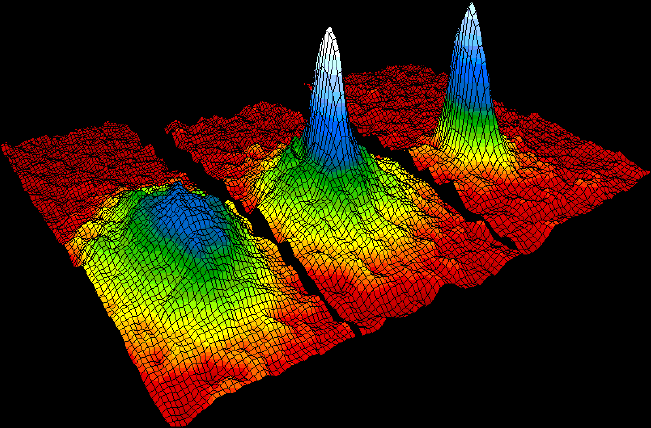
\includegraphics[width=0.7\textwidth]{Fig/Intro/BEC.png}
    \caption[Momentum distribution across Bose-Einstein Condensation]{Bose-Einstein Condensation. As temperature diminishes, the momentum distribution gets increasingly peaked around zero momentum.}
    \label{fig:1st_BEC}
\end{figure}


Last but not least, the momentum distribution also contains signatures of more complex interaction-induced correlation patterns between several individual particles. One of the most simple and famous example of such correlations are opposite momentum pairing effects. This is notably the case for the two electrons in Cooper pair as discussed earlier, as well as for the \textbf{quantum depletion} of a BEC. The quantum depletion designates the fraction of atom removed from the condensate by the effect of interactions and quantum fluctuations and is then a classic and conceptually simple example of a many-body effect. While the quantum depletion has already been observed before \cite{chang2016,lopes2017,xu2006}, there have been no direct observation of the opposite momentum pairing of quantum depleted atoms. Obtaining this result will be the main point of focus of this manuscript.

\section*{Metastable Helium and electronic detection}

Ideally, we would like to characterize all kinds of correlations present in the system, \ie correlations involving an arbitrary amount of particles. This is only achievable if a method is available to measure the momentum of each of the individual atoms of the gas. This is usually not the case in most ultracold experiments where the optical imaging techniques only allow to measure the \textbf{momentum density} of the gas rather than the full \textbf{momentum distribution}. In the early 2000s, the team lead by D. Boiron, C. Westbrook and A. Aspect at Institut d'Optique pioneered a new electronic detection technique exploiting the properties of the metastable state of the Helium atom that they managed to bring to quantum degeneracy in 2001 \cite{robert2001bose}. This detection technique has the amazing advantage of having a \textbf{single-atom} sensitivity, making it perfectly suited for the measurement of correlations in momentum space.

A second metastable Helium experiment was then built at Institut d'Optique under the direction of David Clément starting in 2011, with the observation Bose-Einstein condensation in 2015 \cite{bouton2015fast}. This new experiment implemented a new cooling sequence allowing to produce a BEC in $\sim 6\rm{s}$ instead of $\sim 30\rm{s}$ on the historical experiment, thus significantly speeding up the data acquisition time for momentum correlation measurements.

\section*{Optical lattices and the superfluid-to-Mott insulator transition}

The other specificity of this experiment is the use of optical lattices, from which the name of the team ``Helium Lattice'' derives. Optical lattices are particularly suited to study many-body, strongly interacting systems as the lattice potential locally increases the density and in turn the interactions, making phenomenon like quantum depletion even more pronounced than in regular harmonic traps. In addition, the Bose-Hubbard model predicts the existence of a phase transition from a superfluid phase to an insulating phase when the depth of the lattice potential increases known as the superfluid-to Mott insulator transition, first observed with cold atoms by I. Bloch team in 2002 \cite{greiner2002quantum}. Studying momentum correlations all across the superfluid-to Mott insulator transition sets the general frame of the work presented in this manuscript conducted during my time as an intern and then PhD student in the Helium Lattice team that I the chance to join in 2018.

\section*{Outline of the manuscript}

This manuscript is organized in five chapters. All chapters but the final one are centered around the common topic of the \kmk correlations in the quantum depletion of weakly-interacting lattice Bose gas.

\begin{itemize}
    \item The first chapter is dedicated to presenting the proper formalism to study quantum correlations. The concept of correlation functions is first introduced in the context of Optics and then extended to atomic physics. We then present the main lines of the Bogoliubov theory of the homogeneous weakly-interacting Bose gas and show what the quantum depletion is and where does the \kmk pairing comes from. Finally, we discuss some recent numerical calculations \cite{butera2020} of the correlations in the Bogoliubov theory for trapped systems, before presenting the essential experimental ingredients to observe the \kmk pairs.
    \item The second chapter is also a theoretical one and discusses the Bose-Hubbard model of bosons trapped in a 3D optical lattice. We explain what the superfluid-to-Mott insulator transition is and discuss the conditions under which the in-trap momentum distribution of the gas can be properly measured using a TOF technique, as well a the observability of the \kmk pairs of the quantum depletion in this system.
    \item The third chapter describes our experimental apparatus, namely the sequence used to produce a BEC of metastable Helium and the detection technique. In a second time, we present two experimental measurements aimed at proving the points raised in Chapter \ref{sec:chapter_2}, one proving that we are able to adiabatically prepare an arbitrary state of the Bose-Hubbard model and a second one measuring beyond-mean field two-body collision effects happening during the TOF to prove that they are negligible in usual experimental conditions and therefore not detrimental to our measurement of the momentum distribution. 
    \item The fourth chapter details our experimental observation of the \kmk pairs of the quantum depletion. We describe the numerical procedure to analyze the data and study the characteristics of the experimental correlation signals in light of Bogoliubov theory: width, amplitude and dependency to temperature. We then perform complementary analysis of the data to obtain results leading towards showing the presence of entanglement in our system: we observe a relative number squeezing measurement between modes $\bm{k}$ and $-\bm{k}$, as well as a violation of the Cauchy-Schwarz inequality. Finally, we discuss some preliminary results on the evolution of the correlation signals with momentum $k$.
    \item The fifth and last chapter is separate from the rest of this manuscript and concerns a different project that was lead during this thesis, the measurement of Tan's contact in 1D gases. We first present what Tan's contact is and present some main results of a recent theoretical study \cite{yao2018tan} of the evolution of contact with temperature and interaction strength for trapped 1D bosons, before showing how our experimental apparatus can be adapted for this kind of measurements. We then present the procedure used to extract the contact from the raw experimental data and discuss the first preliminary results and their discrepancy with theory. We conclude by giving a few possible explanations for these discrepancies and discussing what we plan on doing next.
\end{itemize}











% \chapter{Single-atom detection in momentum space}

\section{Metastable Helium}

\section{The experimental setup}

\subsection{Bose-Einstein condensation of mestatable Helium}

\subsection{3D optical lattice}

\subsection{Electronic detection: The Micro Channel Plate Detector}

\section{Two-photon Raman transfer}

\subsection{Principle of the two-photon Raman transfer}

\subsection{Experimental implementation}


% \chapterimage{Fig/Chapter2/mott_cover_2.png}

\chapter{Optical lattices and the Bose-Hubbard model}

\label{sec:chapter_2}

Quantum gases loaded in optical lattices (lattice gases for short) are one of the paramount examples of Quantum Simulation systems. The periodical trapping potential indeed well reproduces the crystal structure of condensed matter system and allows to study relatively simple Hamiltonians such as the Bose-Hubbard Hamiltonian or the Ising model \cite{bloch2005ultracold} that however account for interactions and show strong correlations effects. The main advantages of this experimental platform is that the different parameters of the Hamiltonians are easily set and controlled, while information about the system are relatively easy to access via quantum microscopes \cite{bakr2009quantum} for the in-situ positions of the atoms or Time-Of-Flight experiments to access the momentum distribution as it is the case in this manuscript. The experimental observation of the Superfluid to Mott Insulator transition in 2002 \cite{greiner2002quantum} sparked interest in the community and lead to the development of the field from the early 2000s up until this day.

In this chapter, we will detail the main elements of the Bose-Hubbard theory of lattice gases and briefly study the Superfluid to Mott insulator transition. We will then show how and under which conditions the in-trap momentum distribution of the gas can be accessed through Time-Of-Flight measurements, before drawing the connection with the Bogoliubov theory exposed in Chapter \ref{sec:chapter_1}. The goal of this chapter is to give all the essential points necessary to obtain a system in which the \kmk pairs of the quantum depletion can be experimentally observed, rather than providing a detailled description of Bose-Hubbard physics. For a more thorough study of the Superfluid to Mott Insulator transition with our experimental apparatus, we refer the reader to the manuscript of Cécile Carcy \cite{carcy_these}.




\section{The Bose-Hubbard Model}

We consider a 3D lattice potential with cubic symmetry and spacing $d$:

\begin{equation}
    V(\bm{r})=V_{0}\left[\sin ^{2}\left(\frac{k_{d}}{2} x\right)+\sin ^{2}\left(\frac{k_{d}}{2} y\right)+\sin ^{2}\left(\frac{k_{d}}{2} z\right)\right] + V_{\mathrm{ext}} (x,y,z)
\end{equation}

\noindent where $k_d=\frac{2 \pi}{d}$ is the associated wavevector, $V_0$ the lattice depth. For convenience, $V_0$ is usually expressed in units of recoil energy $V_0 = s E_{\rm{r}}$ with $E_r=h^2/ 8 m d^2$. The term $V_{\mathrm{ext}} (x,y,z)$ denotes a harmonic potential related to the Gaussian shape of the lattice beams. For simplicity of calculations, we will first treat here the homogeneous case $V_{\mathrm{ext}} (x,y,z)=0$.

We consider an ensemble of $N$ atoms that interact with one another with the potential $U_{\rm{int}} ( \bm{r}_1, \bm{r}_2)$ loaded in the lattice potential $V(\bm{r})$. The Hamiltonian of the system writes:

\begin{equation}
    \hat{H}=\sum_{i=1}^{N} \frac{\bm{p}_{i}^{2}}{2 m}+\sum_{i=1}^{N} V\left(\bm{r}_{i}\right) + \sum_{i}^{N} \sum_{j>i}^{N} U_{\text{int}}\left(\bm{r}_{i}, \bm{r}_{j}\right)
    \label{eq:H_lattice_full}
\end{equation}

\subsubsection{Non-interacting lattice gas}

To begin, we will consider that the atoms are non-interacting and study the simplified Hamiltonian:

\begin{equation}
    \hat{H}_0=\sum_{i=1}^{N} \frac{\bm{p}_{i}^{2}}{2 m}+\sum_{i=1}^{N} V\left(\bm{r}_{i}\right)
\end{equation}

\noindent As the Hamiltonian is separable along the 3 directions of space and the gas of atoms is non-interacting, we can simply work with the one-dimensional, single particle Hamiltonian:

\begin{equation}
    \hat{H}_{\rm{1D}} = \frac{p_x^2}{2m} + \sin^2 \Big(\frac{k_d}{2} x \Big)
\end{equation}

\noindent To find the eigenstates of this Hamiltonian, we use the Bloch's theorem \cite{ashcroft1976solid}:

\begin{tcolorbox}[colback=red!5!white,colframe=red!75!black,title=\textbf{Bloch's theorem}]
\label{sec:bloch}
The eigenstates of a Hamiltonian corresponding to a spatially periodic potential $V(\bm{r})$ on a lattice $\mathcal{B}$ are Bloch waves $\psi_{\bm{q}}(\bm{r})$, product of a plane-wave $e^{i \bm{r}.\bm{q}}$ and a periodical function on $\mathcal{B}$, $u_{\bm{q}} (\bm{r})$.
\end{tcolorbox}

We therefore look for eigenstates of the form:

\begin{equation}
    \psi_{n,q} (x)= e^{iqx} u_{n,q} (x)
    \label{eq:bloch_wave}
\end{equation}

\noindent with $n \in \N$ and $q \in \R$ the \textbf{quasi-impulsion}. In order to determine the functions $u_{n,q} (x)$ and the energy $E_n (q)$, we inject equation \ref{eq:bloch_wave} in the eigenvalue equation to find that they must verify:

\begin{equation}
    \left[\frac{\left(p_{x}+\hbar q\right)^{2}}{2 m}+V_{0} \sin ^{2}\left(\frac{k_{a}}{2} x\right)\right] u_{n, q}(x)=E_{n}(q) u_{n, q}(x)
\end{equation}

\noindent As $E_n (q)$ is periodic $E_n (q+k_d)= E_n(q) \ \forall (n,q)$, we can restric the definition interval of $q$ to $[-k_d/2, k_d/2]$ which is called the \textbf{first Brillouin zone}. This equation can be easily numerically solved to obtain $u_{n, q}(x)$ and $E_n (q)$. We plot on Fig.-\ref{fig:bloch_bands} the first five energy bands as a function of $q$ in the first Brillouin zone for various values of the lattice amplitude $V_0$. Interestingly, we see that a gap appears between the different bands as we increase $V_0$. For a 3D lattice, the total energy is the sum of the energies along each direction of the lattice. The first excited band then corresponds to two 1D lowest energy bands and one 1D excited band. In order for the gap to appear, the lattice amplitude must be above $V_0 \simeq 2.2 \ E_{\mathrm{r}}$, whereas it is present at all values of $V_0$ in the 1D case.

\begin{figure}
    \centering
    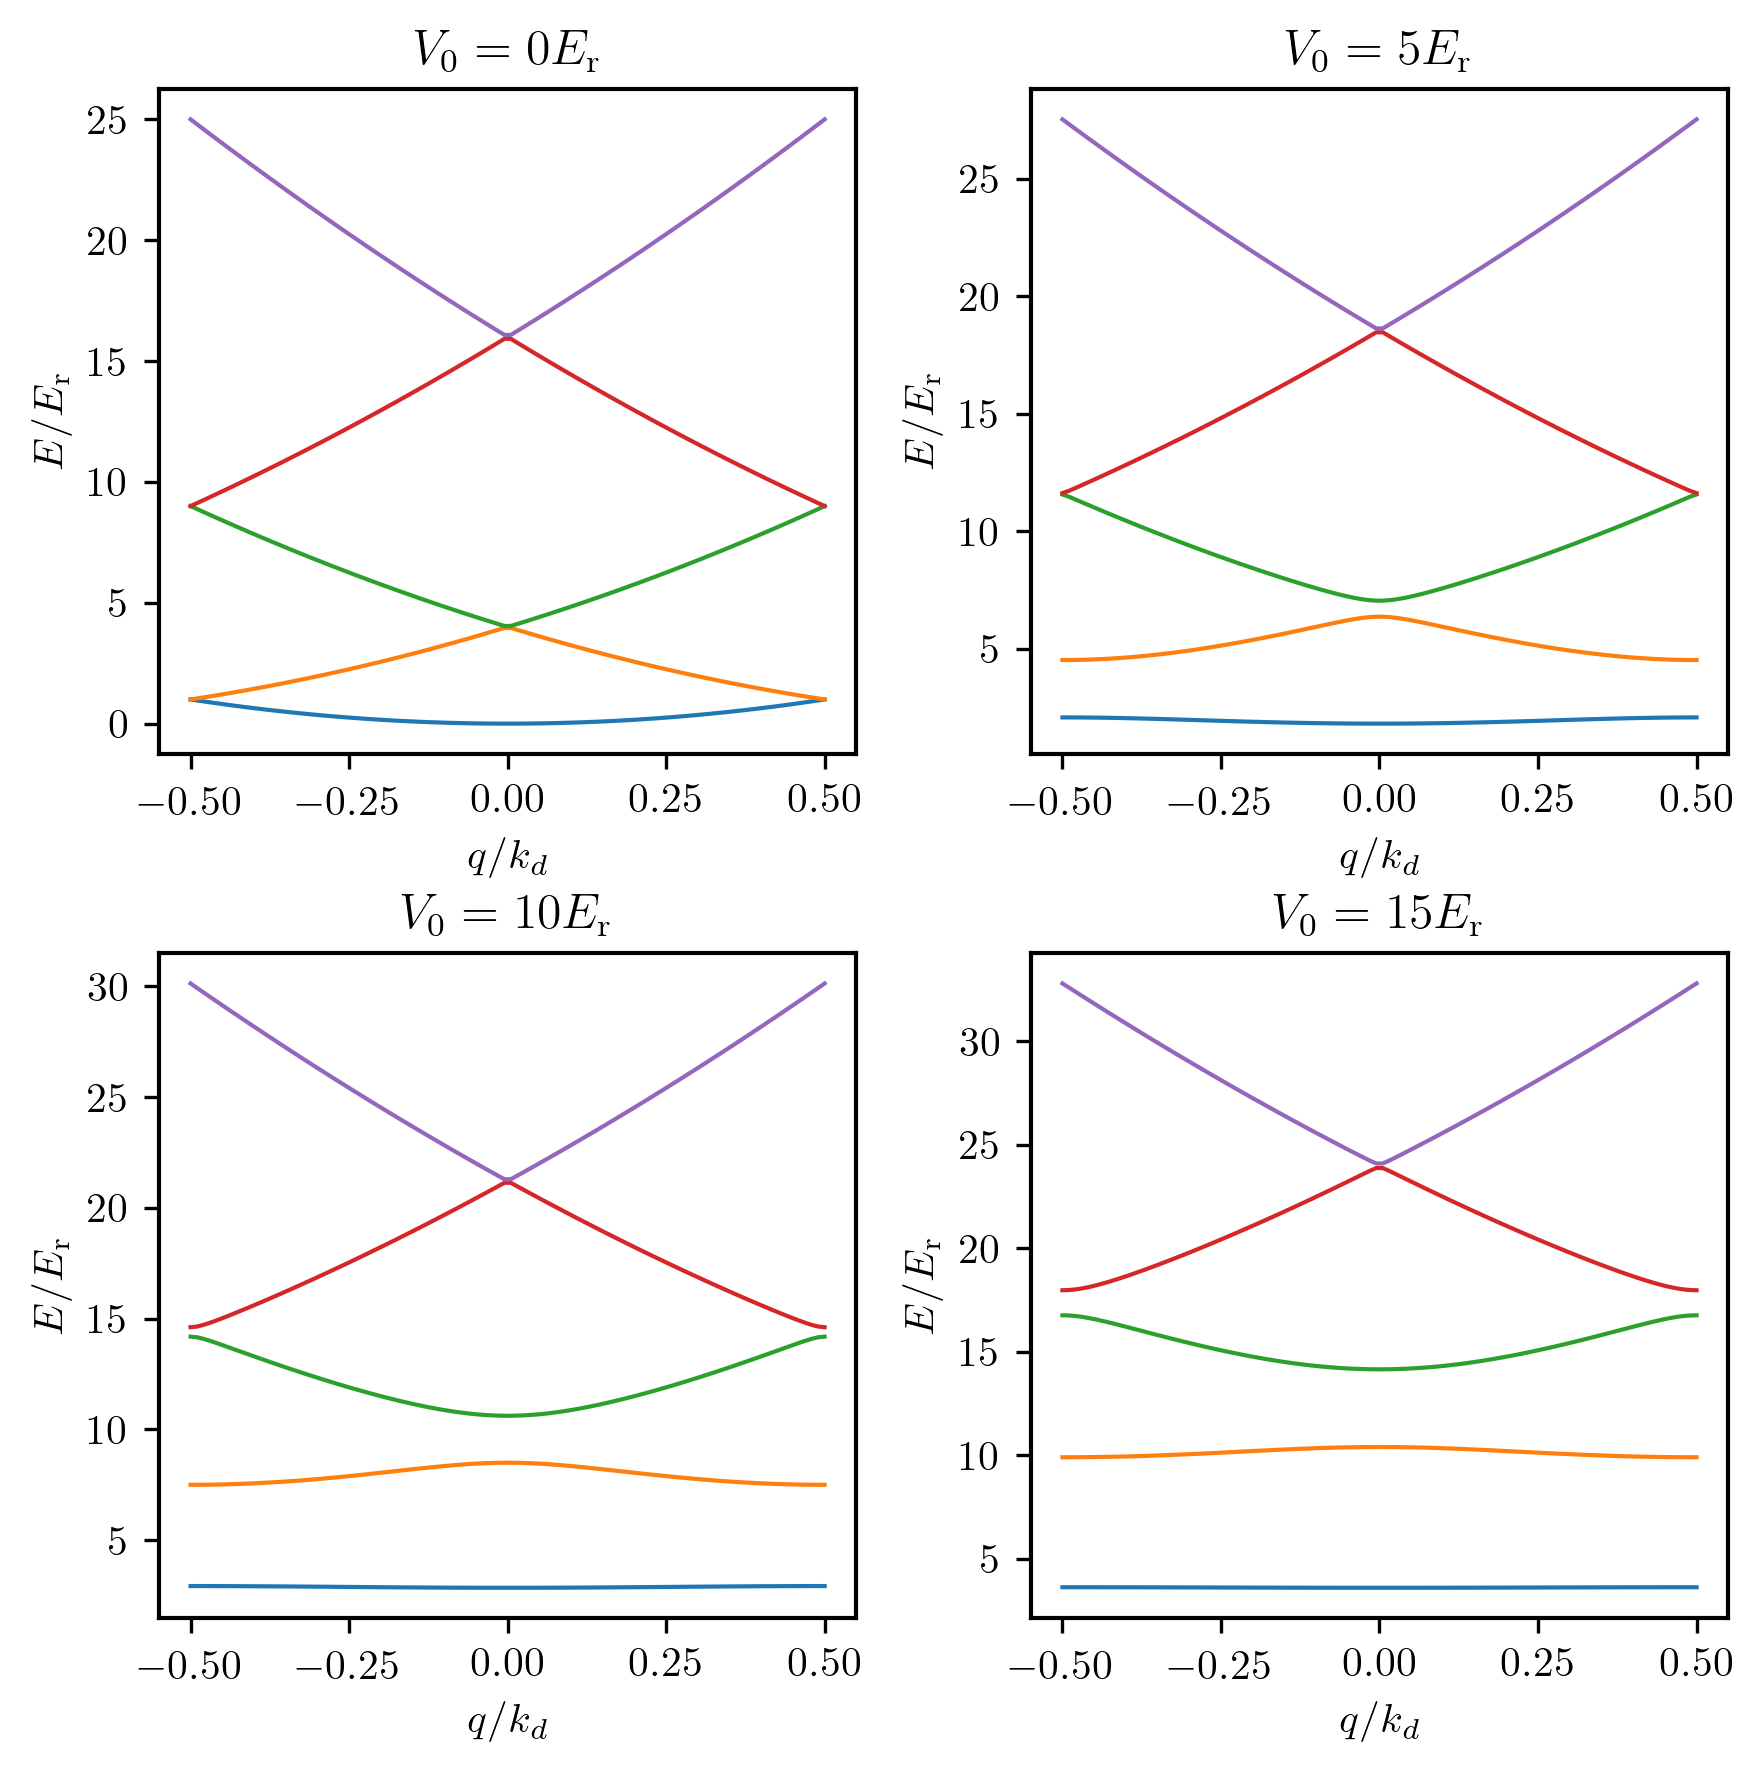
\includegraphics[width=\textwidth]{Fig/Chapter2/bloch_bands.png}
    \caption{First five Bloch energy bands for various lattice amplitudes $V_0$. The gap between the first bands increases as $V_0$ increases.}
    \label{fig:bloch_bands}
\end{figure}

In addition to the Bloch waves, it is possible to define a new kind of functions called the\textbf{ Wannier functions} \cite{wannier1937structure} that are localized near the lattice sites. They are defined from the Bloch waves by:

\begin{equation}
    w_{n, j}(x)=\sqrt{\frac{d}{2 \pi}} \int_{\mathrm{BZ}} \psi_{n, q}(x) e^{-i j q d} \mathrm{~d} q, \quad j \in \mathbb{Z}
    \label{eq:wannier_functions}
\end{equation}

\noindent with BZ denoting an integration over the first Brillouin zone and where $j$ can be interpreted as the index of a lattice site. Actually, we have from equation \ref{eq:wannier_functions} the simple relation:

\begin{equation}
    w_{n, 0}(x-j d)=w_{n, j}(x)
\end{equation}

The Bloch waves can then be re-written with the definition of the Wannier functions and write:

\begin{equation}
    \psi_{n, q}(x)=\left(\frac{d}{2 \pi}\right)^{1 / 2} \sum_{j} w_{n, j}(x) e^{-i j d q}
    \label{eq:bloch_as_wannier}
\end{equation}


\begin{figure}
    \centering
    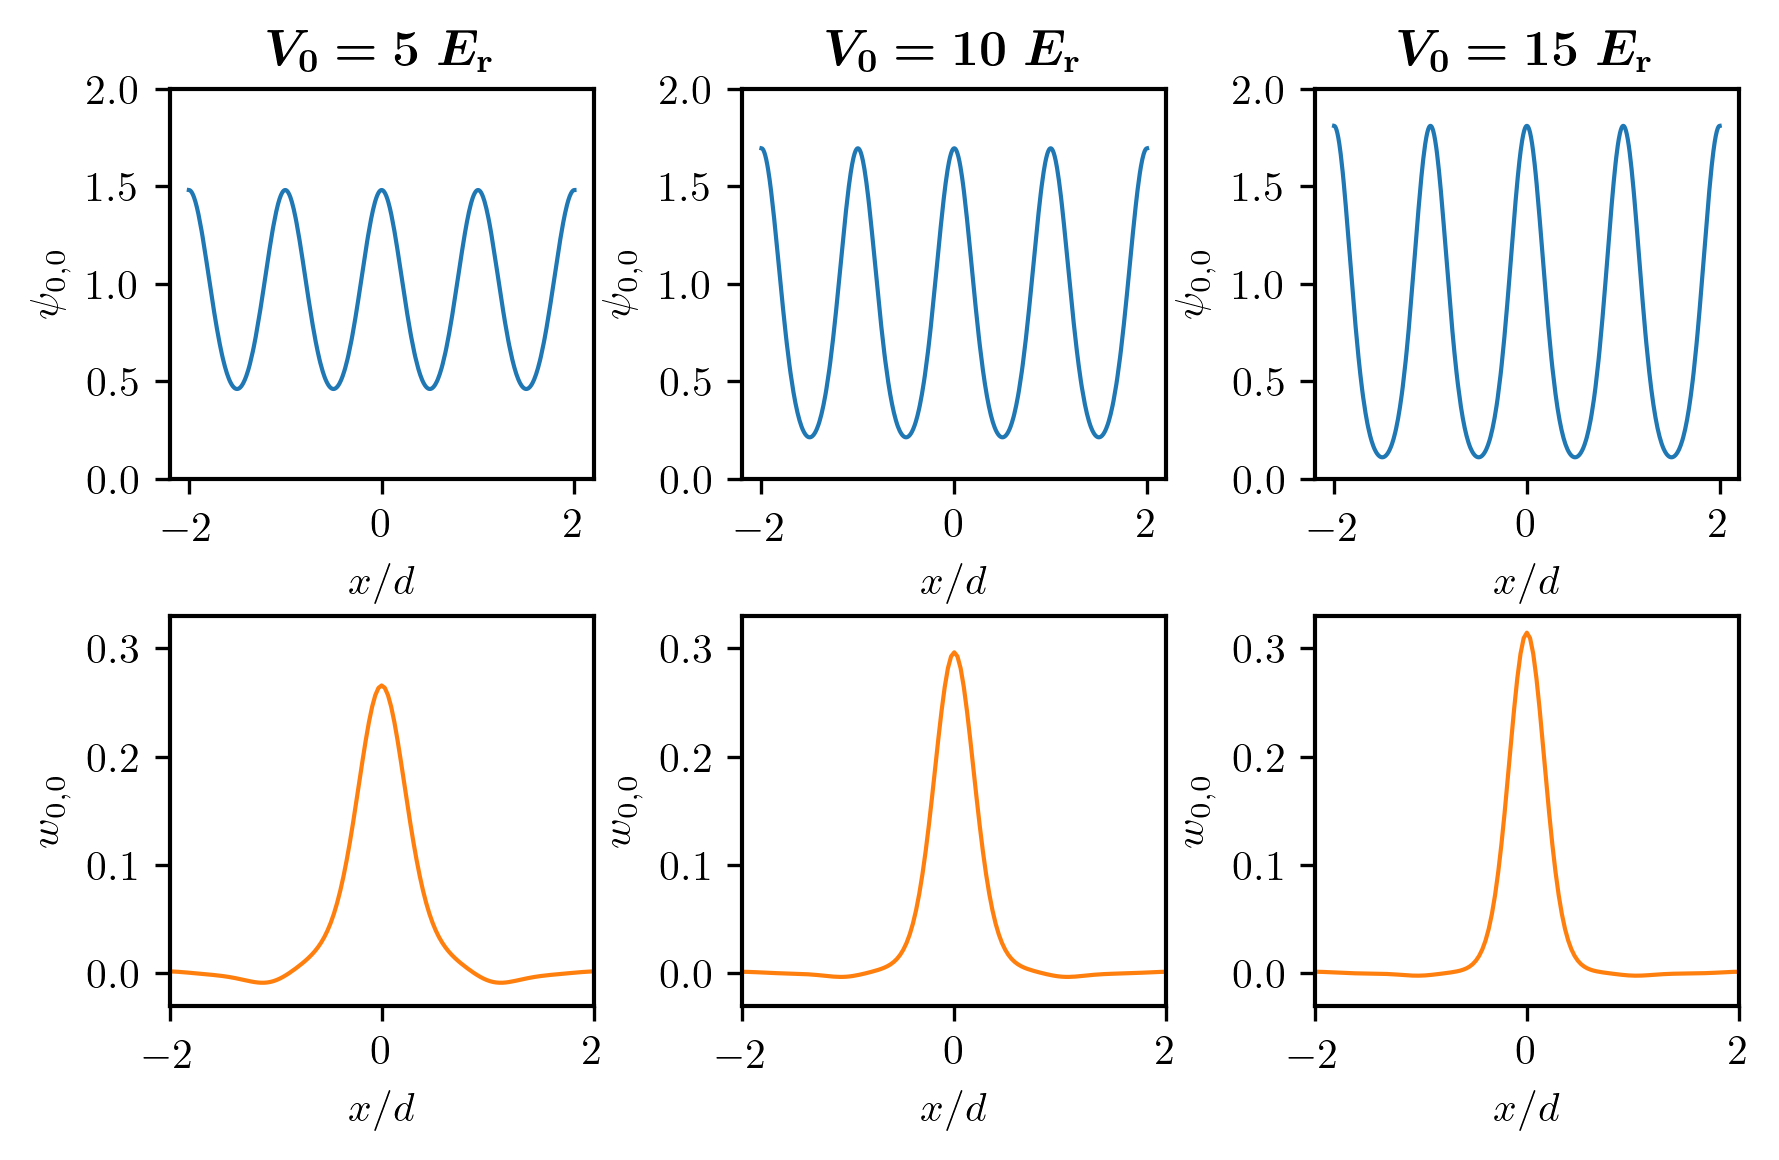
\includegraphics[width=1.05\textwidth]{Fig/Chapter2/bloch_wannier.png}
    \caption{Real parts of the Bloch and Wannier functions for various lattice depths. When the lattice depth increases, the Bloch function is increasingly peaked around the lattice sites and the Wannier function gets narrower.}
    \label{fig:bloch_wannier}
\end{figure}

\noindent The Bloch waves are the sum of the localized Wannier function $w_{n, j}$ that can be interpreted as the wave-function of a particle located in lattice site $j$. The Bloch and Wannier functions for various lattice depths are represented on Fig.-\ref{fig:bloch_wannier}.

We can now re-write the Hamiltonian of the system with the newly introduced Wannier functions. To do so, we start by writing it in the Bloch waves basis with the second quantification formalism, introducing the operator $\hat{c}_{n,q}$ that destroys a particle in the Bloch wave $\psi_{n,q}$.

\begin{equation}
    \hat{H}_{\rm{1D}}=\sum_{n} \int_{\mathrm{BZ}} E_{n}(q) \hat{c}_{n, q}^{\dagger} \hat{c}_{n, q} \mathrm{~d} q
    \label{eq:H_bloch}
\end{equation}

\noindent To change into the Wannier function basis as defined in \ref{eq:bloch_as_wannier}, we introduce the operator $\hat{b}_{n,j}$ destroying a particle in the Wannier function $w_{n,j}$ and defined such as:

\begin{equation}
    \hat{c}_{n}(q)=\sqrt{\frac{d}{2 \pi}} \sum_{j} \hat{b}_{n, j} e^{i j d q}
    \label{eq:a_wannier}
\end{equation}

\noindent Injecting equation \ref{eq:a_wannier} in equation \ref{eq:H_bloch}, we get:

\begin{equation}
    \hat{H}_{\rm{1D}}=\sum_{n} \sum_{j, j^{\prime}} J_{n}\left(j-j^{\prime}\right) \hat{b}_{n, j^{\prime}}^{\dagger} \hat{b}_{n,j}
    \label{eq:H_Jn}
\end{equation}

\noindent This Hamiltonian has a nice physical meaning: it describes the tunneling process by which a particle in site $j$ can ``hop'' to another lattice site $j'$ with the tunneling amplitude $J_n (j-j')$ that writes:

\begin{equation}
    J_{n}\left(j-j^{\prime}\right)=\frac{d}{2 \pi} \int_{\rm{BZ}} e^{i\left(j-j^{\prime}\right) q d} E_{n}(q) \mathrm{d} q
\end{equation}

\noindent This expression tells that the probability for a particle to tunnel from lattice site $j$ to $j'$ is reduced as the distance between the two sites $j$ and $j'$ increases and as the potential barrier, \ie the lattice depth, increases.

As for the rest of this thesis, we will focus ourselves on the ground-state properties of the system and therefore assume that the lowest energy band is the only one populated. This assumption is valid as long as $V_0 \geq 2.2 \ E_{\rm{r}}$ at which the gap is opening. In addition, for $V_0 \geq 3 \ E_{\rm{r}}$, we can use the tight-binding approximation for which only the tunneling events between adjacent sites are non-negligible. We thus simplify the Hamiltonian \ref{eq:H_Jn} by replacing  $J_{n}\left(j-j^{\prime}\right)$ by a constant $J$ denoting the probability to tunnel between adjacent lattice sites that we define as:

\begin{equation}
    J=-J_0(1)
\end{equation}

\noindent so that $J$ is positive. Finally, we obtain the first term of the Bose-Hubbard Hamiltonian:

\begin{equation}
    \hat{H}_{\rm{1D}} = -J \sum_{\mean{i,j}} \hat{b}^{\dagger}_i \hat{b}_j
    \label{eq:H_band}
\end{equation}

\noindent where $\mean{i,j}$ denotes the ensemble of all adjacent lattice sites $i$ and $j$. In the 3D case, the expression of the Hamiltonian remains the same.

\subsubsection{Interaction term}
We now turn to studying the interaction term that we had left out in the full Hamiltonian of equation \ref{eq:H_lattice_full}. In the formalism of second quantification, the short-range, $s$-wave, 1D interaction Hamiltonian writes:

\begin{equation}
    \hat{H}_{\mathrm{int}}=\frac{1}{2} \int d x \int d x' U_{\mathrm{int}}\left(x, x'\right) \hat{\Psi}^{\dagger}(x) \hat{\Psi}^{\dagger}\left(x'\right) \hat{\Psi}\left(x^{\prime}\right) \hat{\Psi}(x)
\end{equation}

\noindent with $\hat{\Psi}(x)$ the operator destroying a particle at position $x$ that we write in terms of Wannier functions as:

\begin{equation}
    \hat{\Psi}(x)=\sum_{j} w_{j}(x) \hat{b}_{j} = \sum_{j} w_{0}(x-x_j) \hat{b}_{j} 
    \label{eq:atom_operator_lattice}
\end{equation}

\noindent Note that we dropped the energy band number $n$ as we are studying the ground-state properties and thus only the lowest energy band. We approximate the interactions to be contact, repulsive interactions so that:

\begin{equation}
    U_{\rm{int}}= g \delta (x_1 - x_2)
\end{equation}

\noindent with $g=\dfrac{4 \pi \hbar^2 a_s}{m}$ the strength of the interactions. The interaction Hamiltonian can then be re-written:

\begin{equation}
    \hat{H}_{\mathrm{int}}=\frac{g}{2} \sum_{j_{1}} \sum_{j_{2}} \sum_{j_{3}} \sum_{j_{4}} \hat{b}_{j_{4}}^{\dagger} \hat{b}_{j_{3}}^{\dagger} \hat{b}_{j_{2}} \hat{b}_{j_{1}} \int w_{j_{4}}^{*}(x) w_{j_{3}}^{*}(x) w_{j_{2}}(x) w_{j_{1}}(x) \mathrm{~d} x
    \label{eq:h_int_intermediate}
\end{equation}

\noindent which is still a fairly complicated expression. We can however greatly simplify it by considering that the Wannier functions become narrower as the lattice depth increases. The overlap between the Wannier functions of the different lattice sites then becomes increasingly negligible. This means that the integral of equation \ref{eq:h_int_intermediate} is non zero only if $j_1=j_2=j_3=j_4$, \ie if we only consider on-site interactions. In the end, the interaction Hamiltonian writes:

\begin{equation}
    \hat{H}_{\rm{int}}=\frac{U_{\mathrm{1D}}}{2} \sum_j \hat{n}_j (\hat{n}_j -1)
\end{equation}

\noindent where we have introduced the on-site energy $U_{\mathrm{1D}}=g \int\left|w_{0,0}(x)\right|^{4} \mathrm{d}x$, easily generalized to the 3D case with $U=g \int(\left|w_{0,0}(x)\right|^{4} \mathrm{d}x)^3$. 

Combining this Hamiltonian to the non-interacting Hamiltonian of equation \ref{eq:H_band}, we reach the form of the famous \textbf{Bose-Hubbard Hamiltonian}:

\begin{equation}
    \hat{H}_{\mathrm{BH}}= -J \sum_{\mean{i,j}} \hat{b}^{\dagger}_i \hat{b}_j + \frac{U}{2} \sum_j \hat{n}_j (\hat{n}_j -1)
\end{equation}

\noindent Interestingly, the physics of the homogeneous ground-state depends only from the two parameters $J$ and $U$ as we will see in the next paragraph. In particular, the ratio $u=U/J$ depends from the lattice depth $V_0$ as illustrated on Fig-\ref{fig:U_J_vs_s}. This parameter is easily controllable in an experiment, for instance by changing the power of the laser beams used to produce the lattice potential. 

\begin{figure}
    \centering
    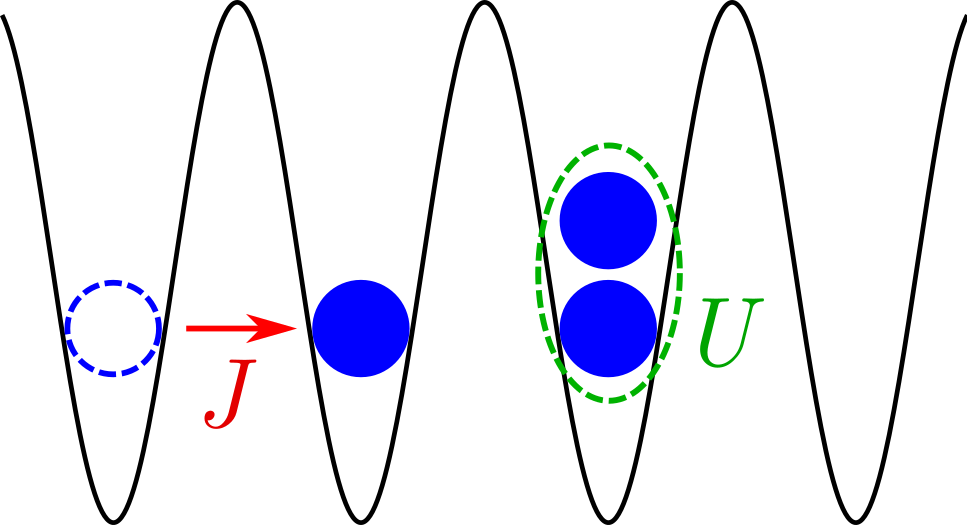
\includegraphics[width=0.5\textwidth]{Fig/Chapter2/illu_bose_hubbard.png}
    \caption{Representation of the Bose-Hubbard model. The physics of the system are set by the tunneling coefficient $J$ and the on-site interaction energy $U$.}
    \label{fig:my_label}
\end{figure}

\begin{figure}
    \centering
    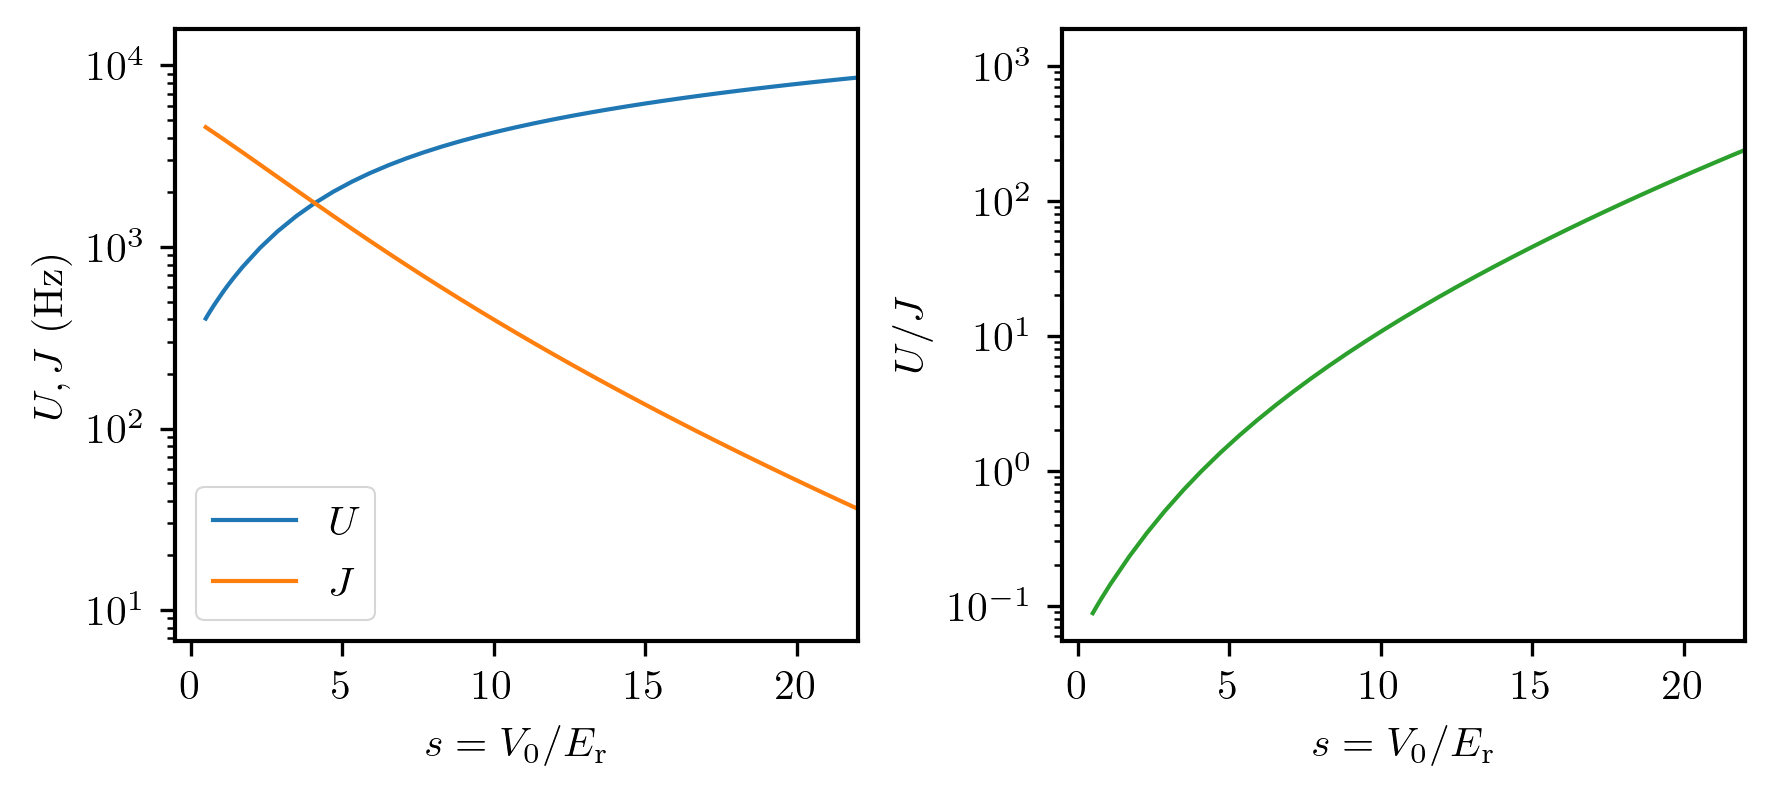
\includegraphics[width=\textwidth]{Fig/Chapter2/U_J_vs_s.png}
    \caption{Evolution of $U$, $J$ and the ratio $U/J$ as a function of the lattice depth in log-scale.}
    \label{fig:U_J_vs_s}
\end{figure}

\section{The superfluid to Mott insulator transition}

We discuss in this section the properties of the Bose-Hubbard Hamiltonian ground-state for $N$ particles spread over $M$ sites with filling $\bar{n}=N/M$. To begin, we describe the extreme cases $u \to 0$ and $u \to \infty$, which are the only cases for which the Hamiltonian can be analytically solved. 

\subsection{Extreme cases}

\subsubsection{Perfect superfluid (SF) phase $\bm{u \to 0}$}

In this case, the particles are non-interacting. In these conditions, the ground-state $\ket{\Psi_0}$ of the N particles system is simply the product of the single particle ground state wave-functions, \ie the Bloch wave-functions for $q=0$ \cite{bloch2008many}:

\begin{equation}
    \ket{\Psi_0}_{\mathrm{SF}} = \frac{1}{\sqrt{N!}} (\hat{c}^{\dagger}(\bm{q}=0))^N \ket{0} = \frac{1}{\sqrt{N !}}\left(\frac{1}{\sqrt{M}} \sum_{j=1}^{M} \hat{b}_{j}^{\dagger}\right)^{N} \ket{0}
\end{equation}

\noindent The ground-state is then an ideal Bose-Einstein condensate with a condensed fraction equal to 1. In the thermodynamic limit with $N \to \infty$, $M \to \infty$, it is possible to show at the price of a few lines of complex calculations \cite{gerbier_notes} that the probability to find $n_i$ atoms at a given site $i$ is:

\begin{equation}
    p\left(n_{i}\right) \approx e^{-\bar{n}} \frac{\bar{n}^{n_{i}}}{n_{i} !}
\end{equation}

\noindent We recognize the same Poissonian distribution that we would obtain for a bosonic coherent state as described in Chapter \ref{sec:chapter_1}. We can therefore write:

\begin{equation}
    \ket{\Psi_0}_{\mathrm{SF}} \approx |\Psi\rangle_{\mathrm{coh}}=\mathcal{N} e^{\sqrt{N} \hat{c}^{\dagger}(\bm{q}=0)} \ket{0} = \mathcal{N} \prod_{i} e^{\sqrt{\bar{n}} \hat{b}_{i}^{\dagger}} \ket{0} = \prod_{i} \mathcal{N}_{i} \sum_{n_{i}=0}^{\infty} \frac{\alpha_{i}^{n_{i}}}{\sqrt{n_{i} !}}\left|n_{i}\right\rangle_{i}
    \label{eq:ground-state_superfluid}
\end{equation}

\noindent with $\alpha_i=\sqrt{\bar{n}} \ \forall i \in \Z$ and the normalization factor $\mathcal{N}_{i}=e^{-\left|\alpha_{i}\right|^{2} / 2}$. We thus find that the ground state can be described as a product of local coherent states associated to the different lattice sites.

As we did in Chapter \ref{sec:chapter_1}, we can write the first-order correlation function between two different lattice sites $i$ and $j$ to characterize the coherence properties of the ground-state:

\begin{equation}
    G^{(1)}(i,j)= \mean{\hat{b}^{\dagger}_i \hat{b}_j}
\end{equation}

\noindent In the limit $U \to 0$, $G^{(1)}(i,j)$ is easy to calculate and writes:

\begin{equation}
    G^{(1)}(i,j)= {}_{\mathrm{SF}} \bra{\Psi_0} \hat{b}^{\dagger}_i \hat{b}_j \ket{\Psi_0}_{\mathrm{SF}} = \alpha^*_i \alpha_j = \bar{n}
\end{equation}

\noindent We see that the result does not depend from the chosen lattice sites $i$ and $j$ and thus from the distance between them, indicating an infinite range coherence.


\subsubsection{Perfect Mott Insulator (MI) phase $\bm{u \to \infty}$}

In the opposite extreme limit, the tunneling probability goes to zero $J=0$ so that each of the lattice sites are independent from one another. The Hamiltonian reduces to:

\begin{equation}
    \hat{H}_{\mathrm{BH}} = \frac{U}{2} \sum_j \hat{n}_j (\hat{n}_j -1)
\end{equation}

Because of the strong repulsive interactions, the particle localize on the lattice sites and cannot hop from site to site as $J=0$. The ground-state is then reached by distributing the particles among the different sites of the lattice so that the number of particles per site is as low as possible to minimize the interaction energy. This corresponds to putting $\bar{n}=N/M$ particles in each of the $M$ available lattice sites. For simplicity sake, we assume here that the filling is commensurate, \ie $\bar{n}$ is an integer. The ground-state then has the simple expression of a Fock state:

\begin{equation}
    \left|\Psi_{0}\right\rangle_{\mathrm{MI}}=\frac{1}{\sqrt{N !}} \prod_{j=1}^{M}\left(\hat{b}_{j}^{\dagger}\right)^{\bar{n}}|0\rangle
    \label{eq:ground-state_MI}
\end{equation}

\noindent This state is called the \textbf{Mott insulator} state \cite{fisher1989boson}. The first-order correlation function now writes

\begin{equation}
     G^{(1)}(i,j)= {}_{\mathrm{MI}} \bra{\Psi_0} \hat{b}^{\dagger}_i \hat{b}_j \ket{\Psi_0}_{\mathrm{MI}} = \delta_{i,j}
\end{equation}

\noindent and is zero when we consider any pair of different lattice sites with $i \neq j$. In the limit $J \to 0$, the system is therefore incoherent.



\subsection{The zero-temperature Mott phase transition}

What can then be said from intermediates values of $U/J$? If we start from the case $J=0$ and progressively start increasing $J$, it becomes possible for the atoms to hop from site to site. When an atom hops to an adjacent site, the occupancy is increased, increasing the energy by $U$. When the gain in kinetic energy $J$ is smaller than $U$, this process is unfavorable and the atoms remain localized on the lattice sites. However, when $J$ is larger than $U$, the gain in kinetic energy outweighs the effect of the interactions and the atoms hop through the different sites of the lattice. The ground-state of the Bose-Hubbard then undergoes a phase transition as $U/J$ varies from an \textbf{insulating phase} to a \textbf{superfluid phase} with very different properties.

\begin{minipage}[t]{0.45\textwidth}
    \noindent \textbf{Superfluid phase}
    \begin{itemize}
        \item The atoms are delocalized over the entire lattice.
        \item The condensed fraction is non zero.
        \item The system shows long range coherence, \ie the phase is fixed.
        \item The on-site number of atoms is fluctuating.
        \item For low values of $u$ far from the transition, the effect of interaction is small, so that we can use the Bogoliubov approximation as we will detail later in this chapter. We find that the excitation spectrum is gapless and phonon-like at low $q$.
    \end{itemize}
\end{minipage}
\begin{minipage}[t]{0.48\textwidth}
    \noindent \textbf{Insulating phase}
    \begin{itemize}
        \item The atoms are well localized on the lattice sites.
        \item The condensed fraction is zero.
        \item The system is incoherent, the phase is fluctuating.
        \item The on-site number of atoms is well defined and non fluctuating.
        \item The excitation spectrum is gapped, with the excitations consisting of particle-hole modes that can restore short-range coherence. 
    \end{itemize}
\end{minipage}

\begin{figure}
    \centering
    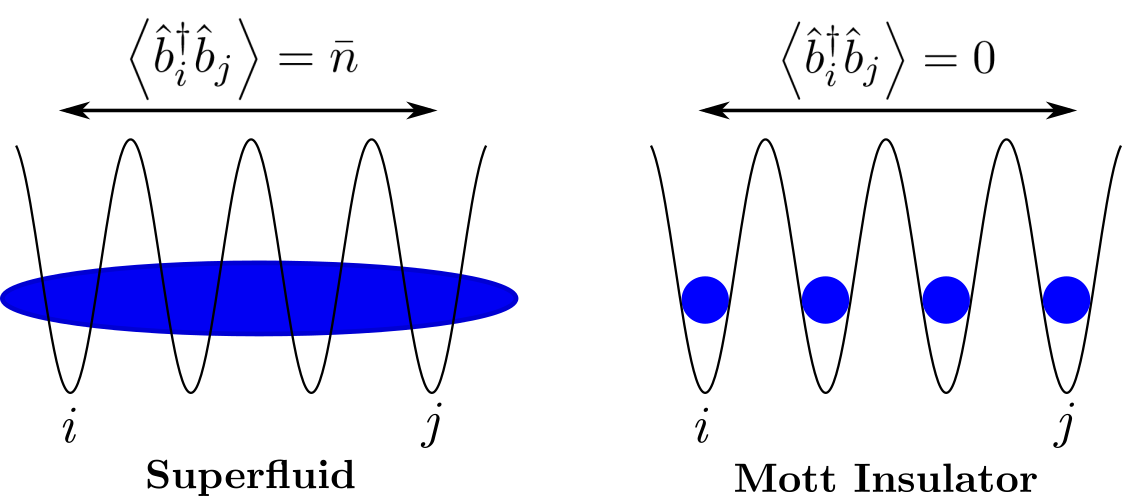
\includegraphics[width=0.9\textwidth]{Fig/Chapter2/schema_superfluid_mott.png}
    \caption{Schematic of the superfluid to Mott insulator transition. In the superfluid phase, the atoms are delocalized and the system shows long range coherence, contrary to the Mott insulator phase where the atoms are well localized on the lattice sites, making the system incoherent.}
    \label{fig:my_label}
\end{figure}

\subsubsection{Phase diagram}

In the homogeneous case, the properties of the system thus change dramatically when $u$ crosses the \textbf{Quantum Critical Point} (QCP) $u_c$. To discuss the value of $u_c$, we slightly complexify our model where we had only considered commensurate fillings, thus fixing the chemical potential that we now set to be a free parameter. We plot on Fig.-\ref{fig:mott_lobes} the full phase diagram function of $\mu/U$, set by the filling in the Mott insulator phase $\bar{n}$ and $J/U$. As the system is homogeneous, the filling $\bar{n}$ is independent of $u$. The grey dashed lines correspond to iso-filling lines for a given value of $\bar{n}$. For commensurate fillings, the iso-filling lines cross the Mott stability lobes at the critical ratio $u_c$ that increases as the filling increases. If the filling is however incommensurate (line $n=1+\varepsilon$), we notice that the system remains in the superfluid phase as long as $J \neq 0$. This is due to the fact that a small fraction of the atoms can delocalize over the whole lattice without being blocked by the interactions $U$ as there will never be two of these particles in the same site as a consequence of the fact that the filling is incommensurate.

\begin{figure}
    \centering
    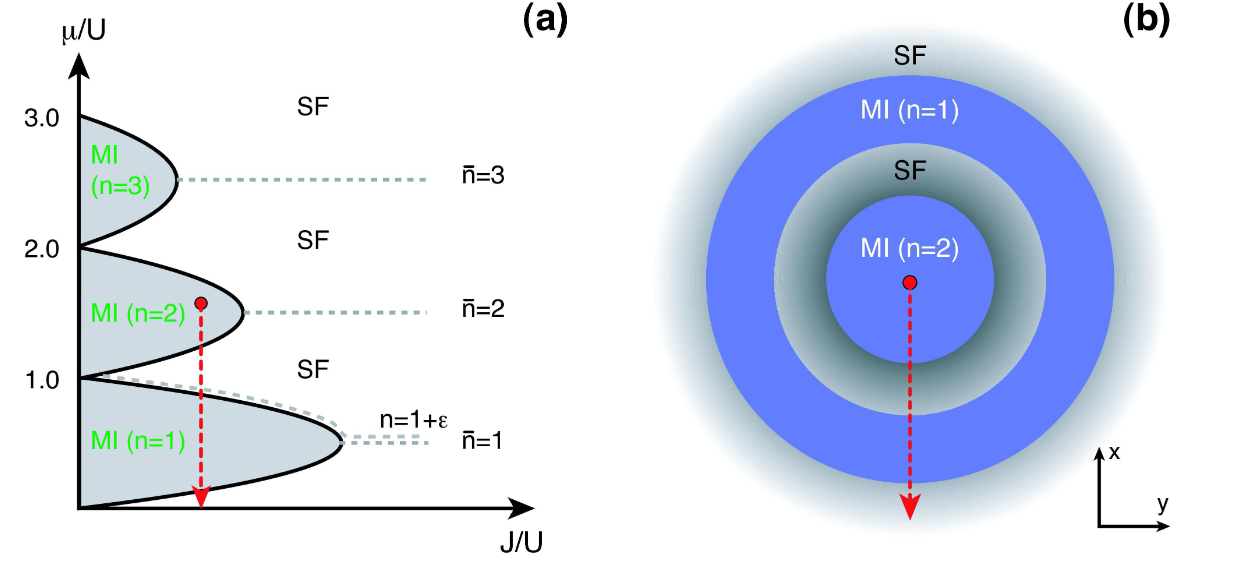
\includegraphics[width=0.9\textwidth]{Fig/Chapter2/mott_lobes.png}
    \caption{(a) Homogeneous phase diagram as a function of $\mu/U$ and $J/U$. The dashed lines are iso-filling lines. We observe a Superfluid to Mott Insulator phase transition for commensurate fillings. (b) Wedding-cake structure for the trapped gas. The red arrow illustrate how $\mu_{\rm{eff}}$ varies and the corresponding phases as the distance from the center of the trap increases. Taken from \cite{bloch2008many}.}
    \label{fig:mott_lobes}
\end{figure}


\subsection{Trapping effects}

\label{sec:ch2_trapping_effects}

In practice, the system is not homogeneous as we require an external harmonic potential $V_{\rm{ext}}(\bm{r})$ to trap the atoms for experiments. The properties of the trapped system can be linked to the properties of the homogeneous system by applying the Local Density Approximation\footnote{Valid as long as the trapping potential varies slowly from site to site and the system is at thermal equilibrium. This approximation may however fail at the quantum critical point \cite{pollet2012recent}.} \cite{bergkvist2004local} and replacing the chemical potential by an effective one:

\begin{equation}
    \mu_{\rm{eff}}= \mu - V_{\rm{ext}}(\bm{r})
\end{equation}

\noindent This means that the effective chemical potential, and thus the lattice filling, varies with the distance from the center of the trap. A typical situation is illustrated by the red arrow on the phase diagram of Fig.-\ref{fig:mott_lobes} where $J/U$ is small enough for Mott phases to exist and the center of the trap corresponds to a filling $\bar{n}=2$. As we get away from the center of the trap towards regions of low $\mu_{\rm{eff}}$ following the red arrow, we exit the first Mott region $\bar{n}=2$ to enter a superfluid region where the filling decreases continuously up to a second Mott region with filling $\bar{n}=1$ and finally reach a last superfluid region at the edge of the trap at vanishing values of $\mu_{\rm{eff}}$. The Mott phases are incompressible, meaning that the density remains constant even though the external trapping potential is rising, differentiating them from the superfluid region. This results in the famous ``wedding-cake'' density profile as illustrated on panel (b) of Fig.-\ref{fig:mott_lobes}.

\noindent For clarity sake, the system will be said to be in the Mott Insulator phase as long as a Mott plateau exists, \ie when $u > u_c$ where $u_c$ is the critical point for the corresponding homogeneous sytem.

\subsection{Finite temperature effects}

If we finally consider the effect of temperature, we obtain the complete phase diagram of Fig.-\ref{fig:phase_diagram} function of $T/J$ and $u$ with the apparition of an additional phase, the normal (thermal) gas. For $u \leq u_c$, the superfluid phase undergoes a condensation transition with temperature similar to the well-known BEC transition. This transition is induced by the thermal fluctuations and is then called classical, in opposition to the Mott transition which is driven by a variations of physical parameters of the Hamiltonian and therefore is a quantum transition. On the other hand, the Mott insulator phase also goes to the normal gas phase as the temperature increases, but with a smooth crossover. Interestingly, the Superfluid to Mott Insulator transition subsists at low temperature. The green area indicates the Quantum Critical Region for which we expect the critical quantum effects of the Mott transition to survive in spite of the temperature. While the physics of the Quantum Critical Point are a very interesting and trending topic, they fall out of the scope of this thesis and we once again refer the reader to \cite{carcy_these} for more informations on this aspect.


\begin{figure}
    \centering
    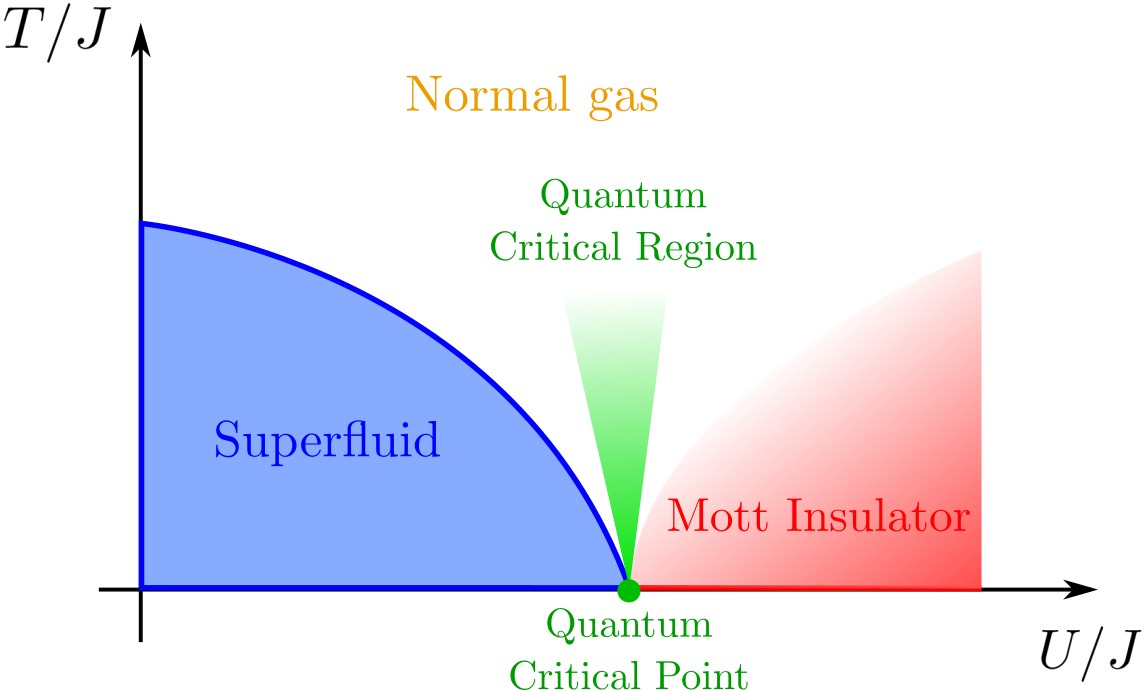
\includegraphics[width=0.78\textwidth]{Fig/Chapter2/phase_diagram.png}
    \caption{Bose-Hubbard phase diagram function of $T/J$ and $U/J$. We identify three phases, the Superfluid, Mott Insulator, and Normal Gas. The green area indicates the region in which critical point quantum effects could be observable in spite of the finite temperature.}
    \label{fig:phase_diagram}
\end{figure}


% The theoretical description of the Bose-Hubbard ground-state at an arbitrary value of $U/J$ is a very challenging task. It however exists a few approximate approaches from which we can obtain meaningful information as we will detail now.

\subsection{The Gutzwiller method}

To conclude this section, we present an approximate theoretical approach to treat the Bose-Hubbard Hamiltonian, the Gutzwiller method. This method takes its name from its author who introduced it in \cite{gutzwiller1963effect} to study strongly correlated Fermi systems. It was later adapted to characterize the ground-state of the Bose-Hubbard Hamiltonian in \cite{rokhsar1991gutzwiller}. This method is particularly useful to evaluate the density profile and therefore the size of the lattice gas with good accuracy all across the Mott transition, apart from the region close to the critical point. Although this is a ground-state, $T=0$ method that does not faithfully represent the reality of experiments, its predictions remain fairly accurate and will be quite valuable to understand the correlation signals that we will present in thesis.

The method revolves around the Gutzwiller ansatz that consists in writing the many-body ground-state as a product of on-site wave-functions $\ket{\phi_i}$:

\begin{equation}
    \ket{\Psi_G} = \prod_i^{\text{sites}} \ket{\phi_i}
\end{equation}

\noindent The on-site wave-functions are then developed on the Fock-state basis:

\begin{equation}
    \ket{\phi_i}= \sum_{n_j=0}^{\infty} f(n_j) \ket{n_j}
\end{equation}

This ansatz is motivated by the fact that it matches the exact ground-state for the extreme cases:

\begin{itemize}
    \item For $u \to 0$, the ground-state is a coherent state (see equation \ref{eq:ground-state_superfluid}) so that $f(n_j) = \mathcal{N}_{j}  (\alpha_{j}^{n_{j}})(\sqrt{n_{j} !})$ with $\alpha_j=\sqrt{\bar{n}}$ and $\mathcal{N}_{i}=e^{-\left|\alpha_{i}\right|^{2} / 2}$.
    \item For $u \to \infty$, the ground-state is already a Fock state (see equation \ref{eq:ground-state_MI}) so that $f(n_j) = \delta_{n_j,\bar{n}}$.
\end{itemize}

The Gutzwiller method is a \textbf{variational} approach, meaning that the ground-state is determined by finding the coefficients $f(n_j)$ that minimizes the free energy defined as:

\begin{equation}
    G = \mean{H_{\mathrm{BH}}}_{\ket{\Psi_G}} - \mu \mean{N}_{\ket{\Psi_G}} = -J \sum_{\langle i, j\rangle} \alpha_{i}^{*} \alpha_{j}+\sum_{j} \sum_{n_{j}=0}^{\infty}\left[\frac{U}{2} n_{j}\left(n_{j}-1\right)-\mu n_{j}\right]\left|f\left(n_{j}\right)\right|^{2}
\end{equation}

\noindent with the condition $\left\langle n_{j}\right\rangle=\sum_{n_{j}=0}^{\infty}\left|f_{j}\left(n_{j}\right)\right|^{2} n_{j}=\bar{n}$. The coefficients $f(n_j)$ can be found through numerical calculations. Interestingly, following the arguments of \ref{sec:ch2_trapping_effects}, $\mu$ can be replaced by the effective $\mu_{\rm{eff}}$ to account for the effect of the external trapping potential present in our experiment.


\section{Accessing the in-trap momentum distribution in a Time-Of-Flight experiment}

\label{sec:ch2_TOF}

Now that we have laid down the main elements of lattice gases physics, we need to determine the proper experimental tools to characterize the system. As developed in Chapter \ref{sec:chapter_1}, the main focus of this thesis will be on the \textbf{momentum space} correlations, requiring us to devise a technique to effectively measure the momentum distribution of a lattice gas. The most natural idea for momentum space measurements is to use the well-known and widely used \textbf{Time-Of-Flight} (TOF) technique. This technique consists in suddenly turning off the trapping potential to let the atoms fall under the effect of gravity and measure their positions $\bm{r}$ after a given TOF $t_{\rm{TOF}}$. In a very simple picture with classical and non-interacting particles, this position gives information about the in-trap momentum of the particle through the simple \textbf{ballistic relation}:

\begin{equation}
    \hbar \bm{k} = \frac{m \bm{r}}{t_{\rm{TOF}}}
\end{equation}

The validity of this simple relation is however far from being obvious for the quantum gases released from optical lattice. We will then describe in this section the TOF dynamics of an atomic gas released from an optical lattice to identify the conditions under which a TOF measurement can be used to properly measure the in-trap momentum of the gas.

% \subsection{The momentum distribution}

% The momentum distribution of a gas of atoms on a homogeneous lattice writes \cite{gerbier2008expansion}:

% \begin{equation}
%     n(\mathbf{k}) \propto |\tilde{w}(\mathbf{k})|^{2} \sum_{i,j} e^{i \mathbf{k} \cdot (\bm{r}_i - \bm{r}_j)} G^{(1)}(i,j)
% \end{equation}

% \noindent where $\tilde{w}(\mathbf{k})$ denotes the Fourier transform of the single site Wannier function. The momentum distribution is thus strongly dependent from the lattice depth. For $U/J \to 0$, $G^{(1)}(i,j) = \bar{n}$ meaning that the momentum distribution consists of sharp peaks located at $k = j k_d$ with $j \in \Z$. In the other limit $U/J \to \infty$, $G^{(1)}(i,j) = \delta_{i,j}$ so that the momentum distribution reduces to $|\tilde{w}(\mathbf{k})|^{2}$, \ie a Gaussian-like function.

\subsection{Expansion from the lattice and Far Field regime}

We start our calculations with the simplified case for which we neglect the effects of all interactions during the TOF. In this configuration, the problem is very similar to the diffraction of a light wave by a grating in optics, in which a diffraction interference pattern results from the coherent sum of the contribution of many source points associated to each of the diffraction grating holes. For the lattice gas, the source points correspond to the lattice sites associated to Wannier functions that will be able to interfere if the system is coherent. For simplicity sake, we will only consider the 1D case from which the 3D case can be easily obtained as the non-interacting Hamiltonian is separable.

At time $t=0$, right before the lattice potential is turned off, the atomic field operator writes (see \ref{eq:atom_operator_lattice})

\begin{equation}
    \hat{\Psi}(x)= \sum_{j} w_{0}(x-x_j) \hat{b}_{j} 
    \label{eq:field_operator}
\end{equation}



\noindent The expression of the Wannier functions is rather complex and very hard to handle in calculations. However, we can approximate the lattice potential near a minimum to its second-order Taylor expansion, \ie approximate it to a harmonic potential of frequency $\omega_L=2 \sqrt{s} (E_{\rm{r}}/\hbar)$ \cite{toth2008theory}. As illustrated in Fig.-\ref{fig:wannier_oh}, this means that the Wannier function can be well approximated by the Gaussian wave-function of the harmonic oscillator ground state:

\begin{figure}
    \centering
    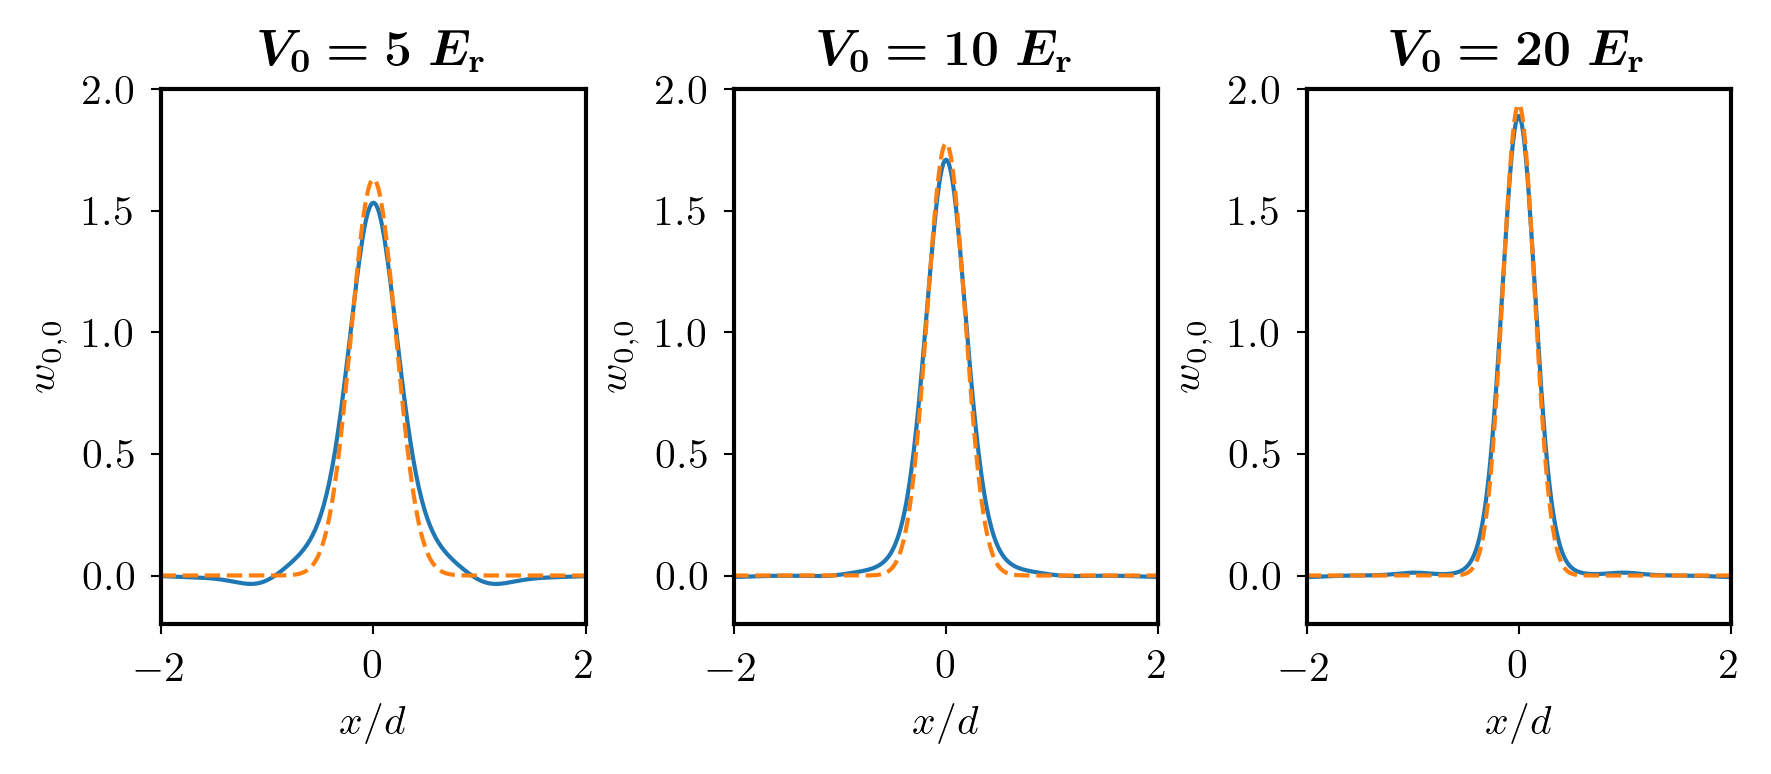
\includegraphics[width=\textwidth]{Fig/Chapter2/wannier_oh.png}
    \caption{Comparison between the Wannier functions (blue) and and the Gaussian wave-function of the harmonic oscillator of frequency $\omega_L$ (orange) for various lattice depths.}
    \label{fig:wannier_oh}
\end{figure}


\begin{equation}
    w_0(x) \simeq \frac{1}{\pi^{1 / 4} \sqrt{x_{0}}} \exp \left(\frac{-x^{2}}{2 x_{0}^{2}}\right)
\end{equation}

\noindent with $x_{0}=\sqrt{\hbar / m \omega_{L}}$.

When the lattice potential is turned off, each of the lattice sites wave-functions expand freely following the harmonic oscillator dynamics \cite{toth2008theory}:

\begin{equation}
    w\left(x-x_{j}, t\right)=\frac{1}{\pi^{1 / 4} \sqrt{W(t)}} \exp \left(-\frac{\left(x-x_{j}\right)^{2}}{2 W(t)^{2}}\right) \exp \left(-i \frac{\left(x-x_{j}\right)^{2}}{2 W(t)^{2}} \frac{h t}{m x_{0}^{2}}\right)
    \label{eq:time_dependent_wannier}
\end{equation}

\noindent with $W(t)=x_{0} \sqrt{1+\left(\hbar t / m x_{0}^{2}\right)^{2}}$ the width of the Gaussian envelope.

\subsubsection{The Far-Field regime}

In practice, as $\omega_L$ is high ($\sim 10^5-10^6 \ \rm{Hz}$), $W(t)$ increases very quickly. For instance, with $s=5$, $W(t)$ is multiplied by $\sim 600$ after $1 \ \rm{ms}$ of expansion and is thus much larger than the size of the lattice $L$. For $t>1 \ \rm{ms}$, we can make the approximation $W(t) \simeq \hbar t/m x_0$ as well as neglect the dependency on the initial site $x_j$ in the amplitude term as long as $|x| \ll W(t)$ so that we can write:

\begin{equation}
    \exp \left(-\frac{\left(x-x_{j}\right)^{2}}{2 W(t)^{2}}\right) \simeq \exp \left(-\frac{x^{2}}{2 W(t)^{2}}\right)
\end{equation}

\noindent This is equivalent to the paraxial approximation of the Fraunhofer diffraction regime in Optics.

Building up on the diffraction analogy, we would like to define an analog Fraunhofer distance where the dependency of the phase factor on the quadratic analog Fresnel term in $x_j$ can be neglected. Using $W(t) \simeq \hbar t/m x_0$, we obtain $\frac{\left(x-x_{j}\right)^{2}}{2 W(t)^{2}} \frac{h t}{m x_{0}^{2}} \simeq \frac{\left(x-x_{j}\right)^{2}}{2 x_0 W(t)}$ from which we derive the condition $\frac{x_j^2}{2 x_0 W(t)} \ll 1, \forall j$ that we rewrite \cite{gerbier2008expansion,toth2008theory}:

\begin{equation}
    t \gg t_{\rm{FF}} = \frac{mL^2}{2 \hbar}
    \label{eq:far_field}
\end{equation}

\noindent This condition defines the \textbf{Far-Field regime} after which the interference pattern is well developed, in analogy to the Fraunhofer regime of diffraction. Combining the different approximations, we simplify \ref{eq:time_dependent_wannier} to:

\begin{equation}
    w\left(x-x_{j}, t\right)=\sqrt{\frac{m}{\hbar t}} \tilde{w_0}[Q(x,t)] \exp\left(-i \frac{\hbar Q(x,t)^{2}}{2 m} \right) \exp\left(i Q(x,t) x_{j}\right)
\end{equation}

\noindent with $Q(x,t)=\frac{m x}{\hbar t}$ and $\tilde{w_0}$ the Fourier transform of the Wannier function. 

Now that we have the general expression of $w\left(x-x_{j}, t\right)$, we generalize it to the 3D case and inject it in equation \ref{eq:field_operator} to obtain the sum of the contribution of each site:

\begin{equation}
    \hat{\Psi} (\bm{r},t) = \left(\sqrt{\frac{m}{\hbar t}} \right)^3 \tilde{w_0}[\bm{Q}(\bm{r},t)] \exp\left(-i \frac{\hbar \bm{Q}(\bm{r},t)^{2}}{2 m} \right) \sum_j e^{i \bm{Q}(\bm{r},t). \bm{r}_{j}} \hat{b}_j
\end{equation}

\noindent From this expression, we finally obtain the atomic density $\rho_{\rm{TOF}}(\bm{r},t) = \mean{\hat{\Psi}^{\dagger} (\bm{r},t) \hat{\Psi} (\bm{r},t)}$ at position $\bm{r}$ and a long TOF $t$:

\begin{equation}
    \rho_{\rm{TOF}}(\bm{r},t) = \left(\frac{m}{\hbar t} \right)^3 |\tilde{w}_0(\bm{Q}(\bm{r},t))|^2 \sum_{i,j} e^{i \bm{Q}(\bm{r},t).(\bm{r}_j - \bm{r}_{i})} \mean{\hat{b}^{\dagger}_i \hat{b}_j }
    \label{eq:rho_tof}
\end{equation}

\noindent The density $\rho_{\rm{TOF}}(\bm{r},t)$ then consists of a smooth envelope $|\tilde{w}_0(\bm{Q}(\bm{r},t))|^2$ set by the Fourier transform of the Wannier function and an interference term $\sum_{i,j} e^{i \bm{Q}(\bm{r},t).(\bm{r}_j - \bm{r}_{i})} \mean{\hat{b}^{\dagger}_i \hat{b}_j }$ that characterizes the coherence properties of the system. A numerical simulation of $\rho_{\rm{TOF}}(\bm{r},t)$ is plotted on Fig.-\ref{fig:sim_expansion} at various expansion time for $s=5$ corresponding to the superfluid phase, illustrating how the interference pattern develops in time.

\begin{figure}
    \centering
    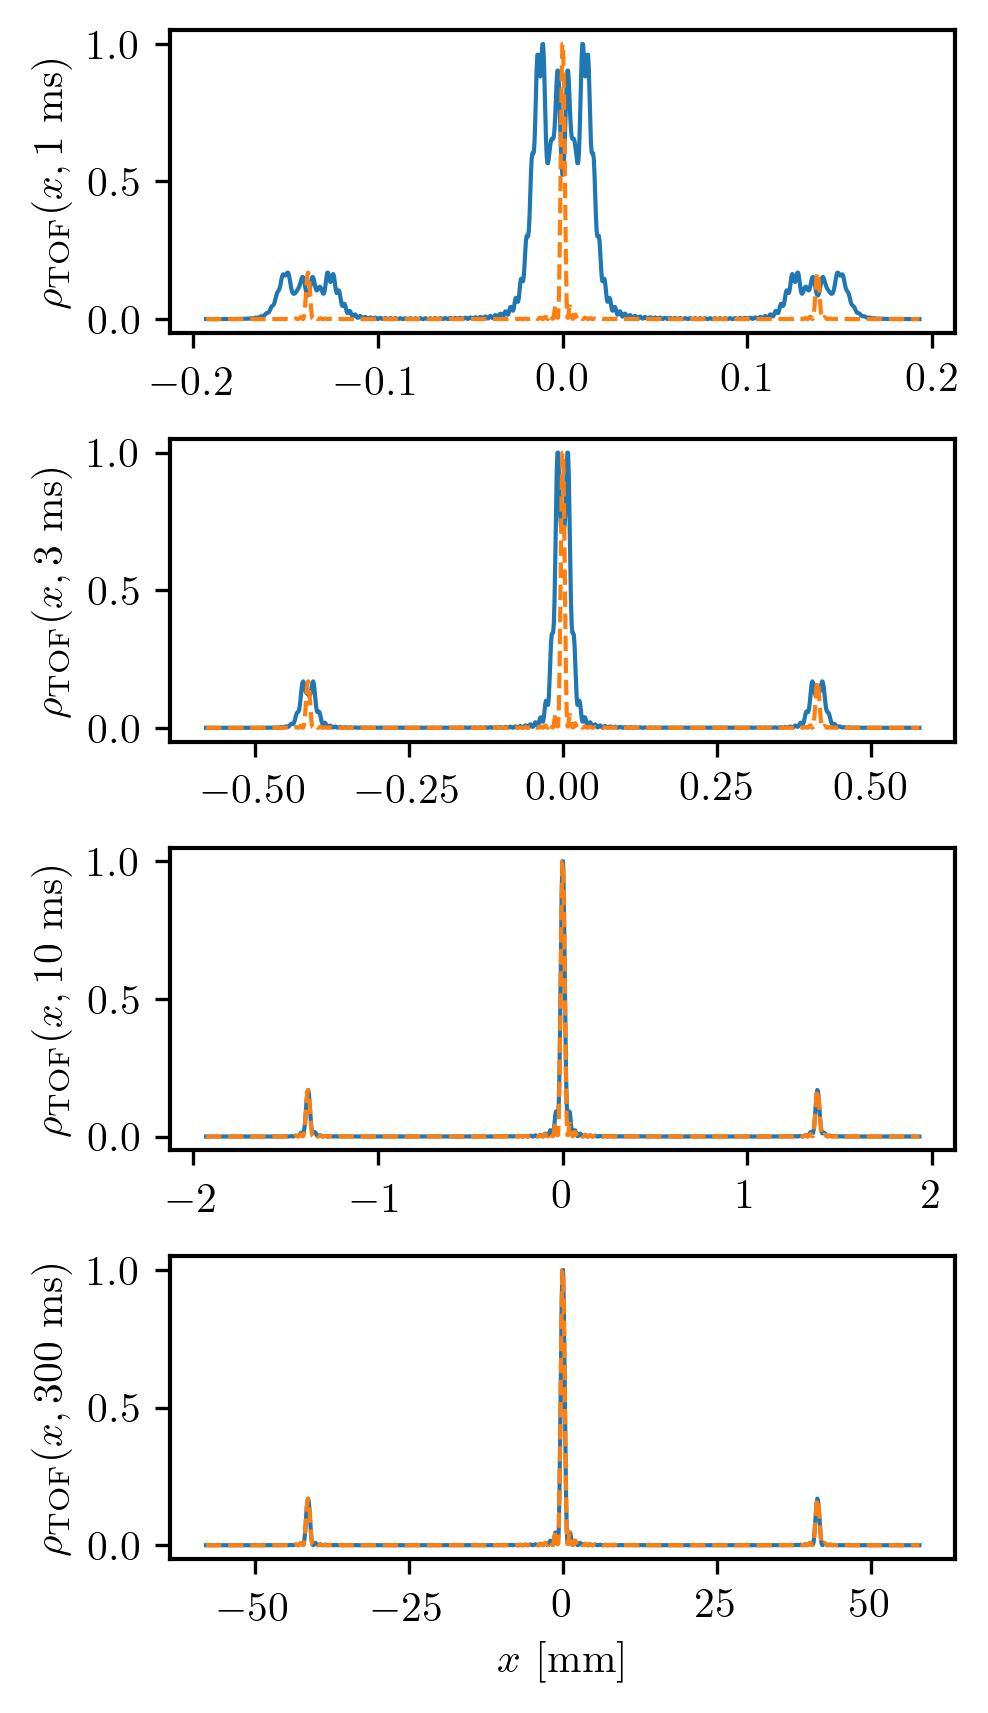
\includegraphics[width=0.7\textwidth]{Fig/Chapter2/TOF_expansion.png}
    \caption{Numerical simulation of the atomic density $\rho_{\rm{TOF}}(x,t)$ after various expansion times from a 1D lattice of 50 sites with $s=5$.}
    \label{fig:sim_expansion}
\end{figure}

\subsubsection{Relation to the momentum distribution}

The main purpose of the TOF technique is to obtain information on the momentum distribution of the gas. To this end, we must find the relation between the measured quantity $\rho_{\rm{TOF}}(\bm{r},t)$ and the in-trap momentum distribution $\rho(\bm{k})$. To do so, we introduce the operator $\hat{a}_{\bm{k}}$ destroying a particle in mode $\bm{k}$:

\begin{equation}
    \hat{a}_{\bm{k}}=\frac{1}{\sqrt{V}} \sum_{j} e^{i \bm{k} \cdot \bm{r}_{j}} \hat{b}_{j}
\end{equation}

\noindent where $V$ is the quantization volume set to be the in-trap volume of the gas. The momentum density then writes:

\begin{equation}
    \rho(\bm{k})=\left\langle\hat{a}^{\dagger}_{\bm{k}} \hat{a}_{\bm{k}}\right\rangle=\frac{1}{V} \sum_{j, i} e^{-i \bm{k} \cdot\left(\bm{r}_{j}-\bm{r}_{i}\right)}\left\langle\hat{b}_{i}^{\dagger} \hat{b}_{j}\right\rangle
    \label{eq:momentum_distribution}
\end{equation}

\noindent If the particle are non-interacting, the ballistic relation gives $\bm{k} = m \bm{r}/\hbar t_{\rm{TOF}}$. From equation \ref{eq:rho_tof}, we obtain:

\begin{equation}
    \rho(\bm{k}) = \frac{\rho_{\rm{TOF}}(\bm{r}=\hbar t\bm{k}/m,t)}{V  \left(\frac{m}{\hbar t} \right)^3 |\tilde{w}_0(\bm{k})|^2}
\end{equation}

In conclusion, under the conditions that there are no interactions during the TOF and $t_{\rm{TOF}} \gg t_{\rm{FF}}$ to be in the far-field regime, the TOF distribution maps the in-trap momentum distribution. 

\subsubsection{Momentum distribution across the Mott transition}

As we have just seen, the momentum distribution is strongly dependent from the coherence properties of the system and in turn of the lattice depth.

\begin{itemize}
    \item In the superfluid phase $u \to 0$, the system is coherent $G^{(1)}(i,j) = \bar{n}$. From equation \ref{eq:momentum_distribution}, we get that the momentum distribution consists of sharp analog diffraction peaks located at $\bm{k} = j k_d \bm{e}_i$ with $j \in \Z$ and $\bm{e}_i$ the unitary vector in direction $i=x,y,z$. In terms of $\rho_{\rm{TOF}}(\bm{r},t)$, the amplitude of the different peaks is set by the Fourier transform of the Wannier function. 
    
    \item In the Mott insulator phase $u \to \infty$ the system is totally incoherent $G^{(1)}(i,j) = \delta_{i,j}$. The momentum distribution is then constant, meaning that $\rho_{\rm{TOF}}(\bm{r},t)$ simply reflects the Fourier transform of the Wannier function, \ie a Gaussian-like function.
    
    \item For intermediate values of $u$, the visibility of the interference pattern progressively decreases as $u$ increases. In addition, as $V_0$ increases, the Wannier function is more and more localized so that the width of its Fourier transform increases. As a result, the population of the diffracted peaks increases with the lattice depth.
\end{itemize}

The experimental quantity $\rho_{\rm{TOF}}(\bm{r},t)$ is therefore a powerful tool to characterize the phase of the system across the Mott transition. This is illustrated on Fig-\ref{fig:mott_greiner} of the first experimental observation of the Mott transition with cold atoms \cite{greiner2002quantum}, on which we can clearly see the visibility of the interference pattern decreasing with $V_0$.

Importantly, a characteristic of the Superfluid to Mott insulator transition is that even though the system is incoherent in the insulating phase, the coherence can be restored by ramping down the lattice depth to the superfluid phase. The standard procedure to characterize the presence of the Mott transition is then to set $V_0$ to be in the superfluid region, ramp up it up to see that the interference pattern disappear, and ramp it down to find back the interference pattern. This allows to certify that the loss of coherence is indeed an effect of the competition between $U$ and $J$ and not an experimental defect, such as unwanted heating of the cloud. 

\begin{figure}
    \centering
    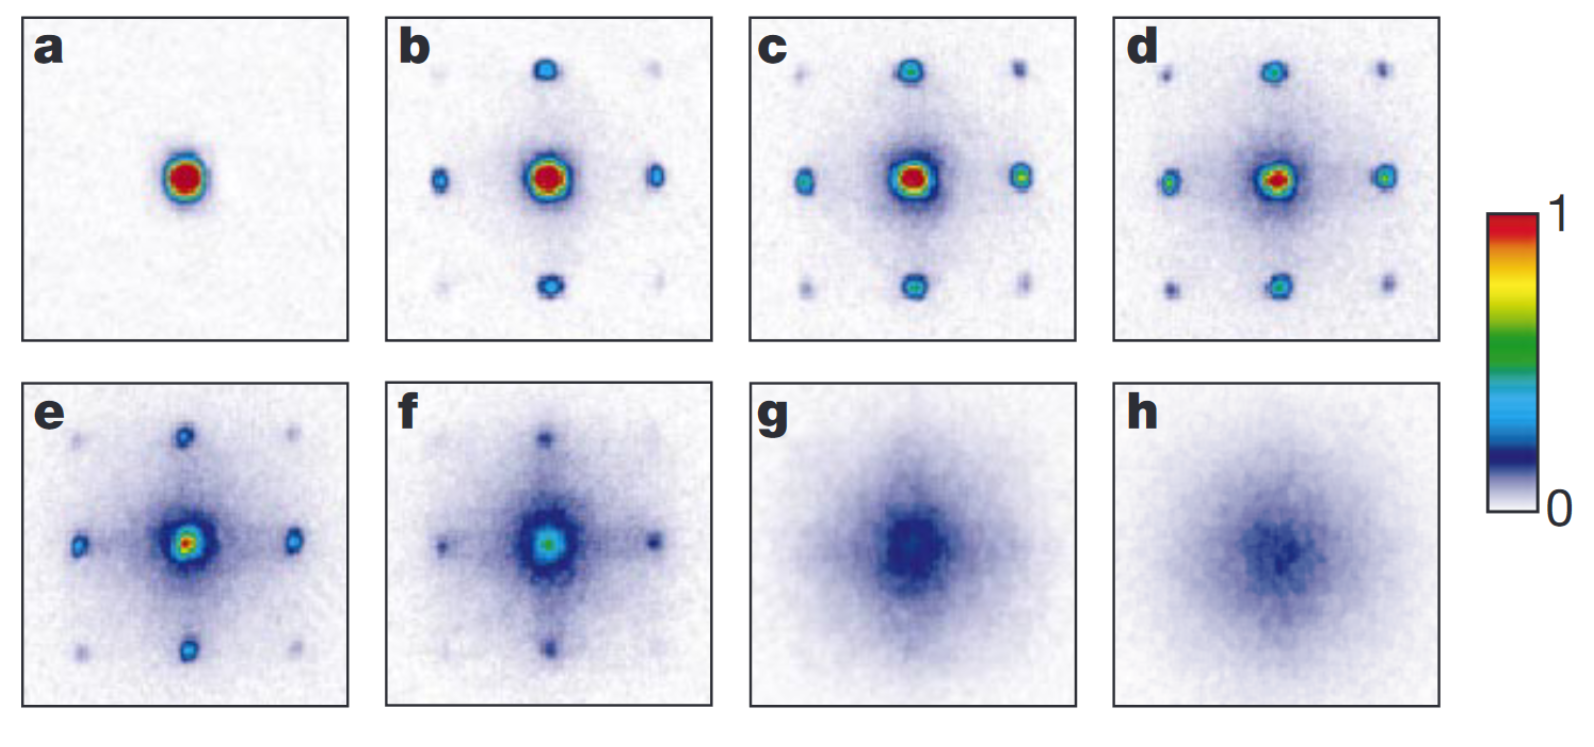
\includegraphics[width=0.9\textwidth]{Fig/Chapter2/mott_greiner.png}
    \caption{Absorption images of Rubidium atoms taken $15 \ \rm{ms}$ after the atoms are released from a 3D cubic lattice. Note that the far-field regime condition is not fulfilled here. \textbf{a)} s=0. \textbf{b)} s=3. \textbf{c)} s=7. \textbf{d)} s=10. \textbf{e)} s=13. \textbf{f)} s=14. \textbf{g)} s=16. \textbf{h)} 20. Taken from \cite{greiner2002quantum}.}
    \label{fig:mott_greiner}
\end{figure}


\subsection{Mean-field interactions}

The experimental technique described in the last paragraph holds if there are no interactions between the particles during the TOF. If it were otherwise, the interactions would affect the TOF dynamics of the gas, preventing us to use the ballistic relation and to map the TOF distribution $\rho_{\rm{TOF}}(\bm{r},t)$ to the in-trap momentum $\rho(\bm{k})$. As interactions cannot be effectively turned off by means of a Feshbach resonance, experimentally inaccessible for $^4 \He$, it is crucial to determine whether interactions during the TOF can be neglected or not and under which conditions.

Describing the interactions between each of the individual particles would be impossible, even for numerical methods for which the calculation time would be prohibitive. To circumvent this issue, the problem can be simplified using the \textbf{mean-field approximation}. The idea is to approximate the effect of the interactions of every atoms on a single one as an \textbf{average} single effect. This considerably simplifies the many-body problem, reducing it to an effective one-body problem.

To quantify the effect of the interactions treated at the mean-field level, we introduce the interaction energy $U_{\rm{int}} \sim gn$ with $g$ the strength of the interactions and $n$ the atomic density. To determine whether the interactions are affecting the expansion of the gas released from the lattice, $U_{\rm{int}}$ must be compared to the zero point energy of the ground-state of the approximate harmonic oscillator associated to a single lattice site, $\hbar \omega_L$. In typical experimental conditions, $U_{\rm{int}}/h \approx 10^3 \ \rm{Hz} \ll \omega_L/2 \pi \approx 10^5-10^6 \ \rm{Hz}$, meaning that the initial expansion is driven by the zero point energy of the lattice and not the released interaction energy. In addition, after a small expansion time, the Wannier functions of the different sites overlap as their width become of the order of the lattice spacing $d$ and might then interact. However, on this time scale, the atomic density is reduced by a factor $(x_0/d)^3 \approx 10^2$ (for $s=10$), meaning that this interaction effect should also negligible \cite{gerbier2008expansion}, provided that the initial density is not too high. This point will be discussed in further details in light of experimental data in Chapter \ref{sec:chapter_3}.

As developed in \cite{kupferschmidt2010role}, the interactions can also induce a dephasing between the different sites. As a matter of fact, the time evolution of the phase of the wave-function associated to a lattice site depends on its initial energy, and therefore of $U_{\rm{int}}$. If the lattice sites have different lattice fillings, which typically is the case in the superfluid phase where the on-site atom number fluctuations are large, the different interfering wave-functions can be dephased from one another, reducing the visibility of the interference pattern. This effect is however also negligible \cite{gerbier2008expansion,kupferschmidt2010role} in the case of our 3D lattice where $a_s \ll x_0$, provided that the filling is not too high.

\subsection{Beyond mean-field interactions}

While the mean-field approximation is efficient to obtain a first understanding on how the interactions might affect the TOF, it is inherently limited as it does not consider interaction effects between several particles. One clearly identifiable beyond mean-field effect happening during the TOF is the presence of scattering halos between the diffraction peaks \cite{greiner2001exploring}. These scattering halos signal the presence of $s$-wave collisions between the atoms of the different diffraction peaks, \ie with significantly different velocities, happening during the first moments of the TOF as they separate. This effect is analog to the scattering halos observed between two colliding condensates \cite{khakimov2016ghost,perrin2007observation,zin2006elastic}.

We have conducted a thorough experimental study of the $s$-wave two-body collisions during the TOF to determine whether they would affect our measurement of the momentum distribution \cite{tenart2020two}. This study will be detailed in Chapter \ref{sec:chapter_3}.

\section{Extension of the Bogoliubov theory to lattice gases}

So far, we have focused on the description of the lattice Hamiltonian under the scope of Wannier functions, culminating in the Bose-Hubbard Hamiltonian describing the physics of the Mott transition. We now wish to go back to the central point developed in Chapter \ref{sec:chapter_1}, namely the \kmk correlations in the quantum depletion predicted by the Bogoliubov theory of the weakly-interacting, homogeneous Bose gas. We concluded by saying that using an optical lattice would be a fitting solution to efficiently increase the interactions as a means to reach the low temperature regime dominated by the interactions $\mu \gg \kB T$ for which we expect the pair correlation signal to be experimentally detectable. This however requires that we extend the method of the Bogoliubov theory to the case of the lattice gas to identify the condition under which the \kmk pairs should be observable.

\subsection{Effect of the lattice amplitude}

As developed in \ref{sec:bogo_approx}, the central point of the Bogoliubov approximation for the weakly-interacting homogeneous Bose gas resides in the fact that the interactions are \textbf{weak}. This means that the system can be described as a BEC from which only a \textbf{small fraction} of the atoms, the depletion, are removed by the effect of interactions.

For the lattice gas, the condensed atoms correspond to the sharp diffraction peaks of the momentum distribution, while the depleted atoms in high quasi-momentum states correspond to the diffuse background between the diffraction peaks that increases as $u$ and therefore the strength of interactions increases, as illustrated by Fig.-\ref{fig:mott_greiner}. We thus need to be in the shallow lattice regime to use the Bogoliubov approximation, \ie at low values of the lattice depth such as $u \ll u_c$. This corresponds to the superfluid phase where the condensed fraction is close to 1 and the fraction of depleted atoms is small.


\subsection{Dispersion relation and effective mass}

For the remainder of this section, we will assume that we are in the shallow lattice regime so that the Bogoliubov approximation can be used. To begin, we remind the Hamiltonian for weakly interacting atoms without the lattice potential, as first introduced in Chapter \ref{sec:chapter_1}:

\begin{equation}
    \hat{H}=\sum_{\bm{k}}\frac{\hbar^2 k^2}{2m} \hat{a}^{\dagger}_{\bm{k}}  \hat{a}_{\bm{k}} +  \frac{g}{2V} \sum_{\bm{k}_1,\bm{k}_2,\bm{k}_3} \hat{a}^{\dagger}_{\bm{k_1}+\bm{k_3}} \hat{a}^{\dagger}_{\bm{k_2}-\bm{k_3}} \hat{a}_{\bm{k_1}} \hat{a}_{\bm{k_2}} 
\end{equation}

\noindent We now add the lattice potential but still neglect the external harmonic trapping potential and write the new Hamiltonian in the Bloch wave basis. In fact, we have already seen the expression of the non-interacting term in the Bloch wave basis in equation \ref{eq:H_bloch}. As we have done throughout this chapter, we consider that only the lowest energy band $n=0$ is populated. The full Hamiltonian writes \cite{dalibard2013cages}:

\begin{equation}
    \hat{H}=\sum_{\bm{q}} E_{0}(\bm{q}) \hat{c}_{\bm{q}}^{\dagger} \hat{c}_{\bm{q}}+\frac{g}{2} \sum_{\bm{q}_{1}, \bm{q}_{2}, \bm{q}_{1}^{\prime}, \bm{q}_{2}^{\prime}} C\left(\bm{q}_{1}, \bm{q}_{2}, \bm{q}_{1}^{\prime}, \bm{q}_{2}^{\prime}\right) c_{\bm{q}_{1}^{\prime}}^{\dagger} c_{\bm{q}_{2}^{\prime}}^{\dagger} c_{\bm{q}_{2}} c_{\bm{q}_{1}}
    \label{eq:lattice_bogo_hamiltonian}
\end{equation}

\noindent with $\hat{c}_{\bm{q}}$ the operator destroying a particle in the Bloch wave $\psi_{0,q}$ and 


\begin{equation}
    C\left(\bm{q}_{1}, \bm{q}_{2}, \bm{q}_{1}^{\prime}, \bm{q}_{2}^{\prime}\right)=\int_{0}^{V} \psi_{0, \bm{q}_{1}^{\prime}}^{*}(\bm{r}) \psi_{0, \bm{q}_{2}^{\prime}}^{*}(\bm{r}) \psi_{0, \bm{q}_{1}}(\bm{r}) \psi_{0, \bm{\bm{q}}_{2}}(\bm{r}) \mathrm{d} \bm{r}
\end{equation}

The non-interacting term $\sum_{\bm{q}} E_{0}(\bm{q}) \hat{c}_{\bm{q}}^{\dagger} \hat{c}_{\bm{q}}$ is quite similar to its equivalent in the homogeneous case $\sum_{\bm{k}}\frac{\hbar^2 k^2}{2m} \hat{a}^{\dagger}_{\bm{k}}  \hat{a}_{\bm{k}}$. In fact, as we can see on Fig-\ref{fig:dispersion_relation_harmonic}, the function $E_{0}(\bm{q})$ can be well approximated by a parabolic function at low values of $q$. We then rewrite $E_{0}(\bm{q})$ as:

\begin{equation}
    E_{0}(\bm{q}) \approx \frac{\hbar^2 q^2}{2 m^*}, \ \text{with } \frac{1}{m^*} = \frac{1}{\hbar^2} \frac{\mathrm{d}^2 E_0 }{\mathrm{d}q^2}
\end{equation}

\noindent where we have introduced the notion of effective mass $m^*$ defined from the curvature of the Bloch energy band, actually very useful to study the dynamics of particles in a lattice potential \cite{kramer2002macroscopic,dalibard2013cages}. Under this form, the non-interacting term of the lattice Hamiltonian is then of the exact same form as for the homogeneous Hamiltonian, the effect of the lattice being contained in the new effective mass $m^*$.

\begin{figure}
    \centering
    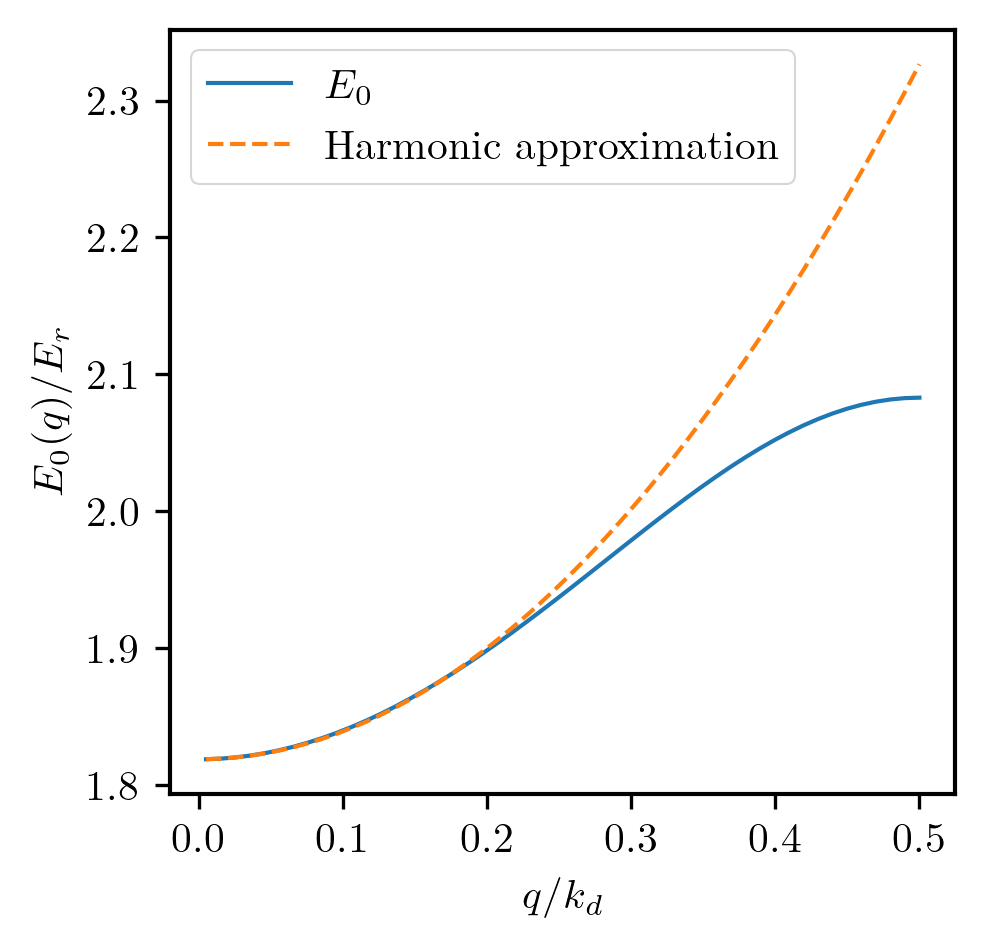
\includegraphics[width=0.5\textwidth]{Fig/Chapter2/dispersion_relation_harmonic.png}
    \caption{Harmonic approximation of the dispersion relation of the first energy band $E_0$ for $s=5$.}
    \label{fig:dispersion_relation_harmonic}
\end{figure}

\subsection{The rescaled interaction strength}

\label{sec:rescaled_interaction}

We turn to calculating the interaction term in equation \ref{eq:lattice_bogo_hamiltonian}. First, like in the homogeneous case, the conservation of momentum gives the relation:

\begin{equation}
    \bm{q_1} + \bm{q_2} = \bm{q}'_1 + \bm{q}'_2
\end{equation}

\noindent allowing us to reduce the sum on $\bm{q}_1,\bm{q}_2, \bm{q}'_1, \bm{q}'_2$ to a sum on three quasi-momenta $\bm{q}_1,\bm{q}_2$ and $\bm{q}_3$. Using the Bloch function form $\psi_{n,q} (x)= e^{iqx} u_{n,q} (x)$ and assuming that only the states at the bottom of the band are populated, we can finally approximate the Hamiltonian \ref{eq:lattice_bogo_hamiltonian} to \cite{dalibard2013cages}:

\begin{equation}
    \hat{H} \approx \sum_{q} \frac{\hbar^{2} q^{2}}{2 m^{*}} \hat{c}_{q}^{\dagger} \hat{c}_{q}+\frac{g^{\prime}}{2 V} \sum_{\bm{q_{1}}, \bm{q_{2}}, \bm{q_{3}}} \hat{c}^{\dagger}_{\bm{q_1}+\bm{q_3}} \hat{c}^{\dagger}_{\bm{q_2}-\bm{q_3}} \hat{c}_{\bm{q_1}} \hat{c}_{\bm{q_2}} 
\end{equation}

\noindent with $g'$ the rescaled interaction strength defined as:

\begin{equation}
    g' = g \left(d \int_0^d |u_{0,0} (x)|^4 \mathrm{d}x \right)^3
\end{equation}

\noindent As long as $V_0 > 0,$ we have $g' > g$ signaling that the lattice indeed increases the strength of the interactions. Importantly, $g'$ increases with $V_0$ as the atoms become increasingly localized in smaller region of spaces, increasing the strength of the interactions.

In conclusion, we obtain an Hamiltonian of the same form than the homogeneous case, with two notable differences:

\begin{itemize}
    \item We have replaced the mass $m$ by the effective mass $m^*$ in the dispersion relation.
    \item The interaction strength $g$ has been replaced by the rescaled and higher interaction strength $g'$.
\end{itemize}

We have then achieved the objective set at the beginning of this chapter, namely obtain a system with \kmk paired quantum depleted atoms as described by the Bogoliubov theory of the weakly-interacting Bose gas, but with increased interactions so that we should be able to reach the low temperature regime dominated by interactions $\kB T \ll \mu$ for which the \kmk correlation signal should be detectable. 

Importantly, the predictions of the Bogoliubov theory detailled in Chapter \ref{sec:chapter_1} should not be taken at face value for the much more complicated system of the inhomogeneous lattice gas. In fact, there have not been clear experimental studies testing the validity of the Bogoliubov approach for this kind of system. It will then be of great interest to compare the predictions of the simple homogeneous case to the experimental data as a means to detect whether the Bogoliubov approach fails or not and under which conditions.





% \chapter{Quantum correlations in the weakly-interacting Bose gas}

\section{Correlation functions}

\subsection{Classical example : HBT with chaotic light}

\subsection{HBT with the perfect Bose gas}

\section{Bogoliubov theory of the weakly-interacting gas}

\subsection{Bogoliubov approximation}

\subsection{Spectrum of excitations}

\subsection{The quantum depletion}

\section{HBT with interacting atoms}

\section{k/-k correlations in the many-body ground-state}

\chapterimage{Fig/Chapter4/goutte_only_transparent.png}

\chapter{Experimental observation of k/-k correlations in the depletion of a weakly-interacting Bose gas}

\label{sec:chapter_4}

The weakly interacting Bose gas has been the subject of a large variety of experimental studies, both aiming at measuring the Bogoliubov spectrum of excitations \cite{fontaine2018,miller1962,ozeri2005,stepanov2019} as well as the quantum depletion \cite{chang2016,lopes2017,xu2006observation}. However, even though there have been experimental measurements of the Lee, Huang and Yang beyond-mean field correction to the ground-state energy \cite{navon2010equation,skov2021observation}, an experimental study of the correlations in the many-body ground-state, and more precisely the observation of the \kmk pairs, is yet to be done more than 60 years after their prediction \cite{lee1957}. As we have seen through the different chapters of this thesis, our experimental setup is perfectly suited for such an investigation. 

We will present in this chapter the main result of this thesis, namely the observation of the \kmk pairs of the quantum depletion \cite{tenart2021observation}. We will detail the numerical procedure and the analysis method used to extract the correlation signals and present the experimental results. With the theoretical developments of Chapter \ref{sec:chapter_1}, we will show how we can link the measured anomalous correlation signal to the \kmk pairs of the quantum depletion by studying the effect of temperature, the widths and amplitudes of the correlation peak, as well as the fluctuations of the atom number difference between modes $\bm{k}$ and $-\bm{k}$. In addition, we will show how our measurement constitutes a first step towards showing the presence of momentum-space entanglement in many-body equilibrium states. We will finally discuss some preliminary results on the evolution of the correlation signals with the region of momentum-space they are probed in.

\section{Numerical procedure to extract two-body correlations}

\label{sec:numerical_calculation}

As seen in the previous chapter, we are capable for each experimental run of reconstructing the 3D momentum coordinates of every atom detected by the $\He$ detector. We must now devise a numerical procedure to extract the two-body correlation signals from this raw data. Our goal is then to compute the general normalized second-order correlation function:

\begin{equation}
    g^{(2)} (\bm{k},\bm{k'}) = \frac{\mean{\hat{a}^{\dagger}_{\bm{k}} \hat{a}^{\dagger}_{\bm{k'}} \hat{a}_{\bm{k}} \hat{a}_{\bm{k'}}}}{\mean{\hat{a}^{\dagger}_{\bm{k}} \hat{a}_{\bm{k}}} \mean{\hat{a}^{\dagger}_{\bm{k'}} \hat{a}_{\bm{k'}} }}
\end{equation}

\noindent We recognize that $\mean{\hat{a}^{\dagger}_{\bm{k}} \hat{a}_{\bm{k}}}$ is the momentum density $\rho(\bm{k})$ in mode $\bm{k}$. We remind the result of Chapter \ref{sec:chapter_1} for weakly-interacting bosons that the $\gtwo$ function will take values different from 1 in two cases:

\begin{itemize}
    \item For $\bm{k'} \simeq \bm{k}$, the \textbf{normal} correlations corresponding to the Hanbury Brown and Twiss effect also known as bosonic bunching.
    \item For $\bm{k'} \simeq -\bm{k}$, the \textbf{anomalous} correlations signalling \kmk pairs in the quantum depletion.
\end{itemize}

In practice, plotting the $\gtwo$ function is not straightforward. On the one hand, the function here is 6D and thus hard to plot in an intelligible way. On the other hand, obtaining a sufficient signal-to-noise ratio for correlation measurements between single modes $\bm{k}$ and $\bm{k'}$ whose volume is typically $(1/L_{\rm{BEC}})^3$, with $L_{\rm{BEC}}$ the size of the BEC, is hardly possible. The idea is then to average the $\gtwo$ function over a large volume $\Omega_k$ of the momentum-space and introduce a new parameter $\delta \bm{k}$ to write:

\begin{equation}
    g_{A}^{(2)} (\delta {\bm k})=\frac{\int_{\Omega_{k}} \langle \hat{a}^{\dagger}_{\bm k} \hat{a}^{\dagger}_{\delta {\bm k} - {\bm k}} \hat{a}_{\bm k} \hat{a}_{\delta {\bm k} - {\bm k}} \rangle \mathrm{d}{\bm k}}{\int_{\Omega_{k}} \rho(\bm k) \rho(\delta {\bm k} - {\bm k}) \mathrm{d}\bm{k}}
    \label{Eq:g2_anomalous}
\end{equation}

\begin{equation}
    g_{N}^{(2)} (\delta {\bm k})=\frac{\int_{\Omega_{k}} \langle \hat{a}^{\dagger}_{\bm k} \hat{a}^{\dagger}_{\delta {\bm k} + {\bm k}} \hat{a}_{\bm k} \hat{a}_{\delta {\bm k} + {\bm k}} \rangle \mathrm{d}{\bm k}}{\int_{\Omega_{k}} \rho(\bm k) \rho(\delta {\bm k} + {\bm k}) \mathrm{d}\bm{k}}
    \label{Eq:g2_normal}
\end{equation}

\noindent With this definition, we see that for $\delta \bm{k}=\bm{0}$, we are either looking at \textbf{anomalous} \kmk correlations (equation \ref{Eq:g2_anomalous}) or \textbf{normal} \kk correlations (equation \ref{Eq:g2_normal}). Note that the absence of a subscript $(N,A)$ in the following denotes a general calculation valid for both normal and anomalous correlation functions. We reduced the 6D function to a 3D function of the parameter $\delta \bm{k}$ which equals $\bm{0}$ when the correlation condition $\bm{k'} = \pm \bm{k}$ is fulfilled. This gives us a natural way to evaluate $\gtwo (\delta \bm{k})$ with the experimental data: we compute the values of the parameter $\delta \bm{k}$ for every detected atom pairs in an experimental run by calculating their momentum sum or difference for anomalous and normal correlations respectively. By computing the histogram of these values and averaging over many experimental runs, we evaluate the numerator of equation \ref{Eq:g2_anomalous} or \ref{Eq:g2_normal} respectively.

\subsection{Description of the algorithm}

The algorithm described here is similar to the one used in our previous works \cite{carcy2019momentum,cayla2020} and detailed in \cite{carcy_these,cayla_these}. This previous version was mainly designed for the observation of bosonic bunching. I adapted the algorithm to make it suitable for the calculation of \kmk correlations as well, as we will discuss now.

\subsubsection{Numerator calculation}

The first step is to compute the numerator of equations \ref{Eq:g2_anomalous} or \ref{Eq:g2_normal} that we denote $G^{(2)}(\delta \bm{k})$. We note $N_{\rm{runs}}$ the number of experimental runs and $N_{i}$ the number of atoms in the $i$-th shot. The procedure is as follows:

% \begin{algorithm}
% \caption{$G^{(2)}$ calculation}
%     \begin{algorithmic}{}
%         \FOR{$i=1:N_{runs}$}
%             \FOR{$j=1:N_{i}$}
%                 \STATE Compute $\vec{k}_i+\vec{k}_j$
%                 \STATE Increment histogram $G^{(2)}$ corresponding pixel
%             \ENDFOR
%         \ENDFOR
%     \end{algorithmic}{}
% \end{algorithm}


\begin{algorithm}[h!]
 \caption{$G^{(2)}$ calculation}
    \begin{algorithmic}
         \For{$i=1:N_{\rm{runs}}$}
            \For{$j=1:N_{i}$}
               \For{$p=1:N_{i}$}
                    \State Compute $\delta \bm{k} = \bm{k}_j \pm \bm{k}_p$
                    \State Increment the corresponding voxel in 3D histogram $G^{(2)}$ 
                \EndFor
            \EndFor
        \EndFor
\end{algorithmic}

\end{algorithm}

\noindent We end up with a 3D histogram where each voxel is associated to a value of $\delta \bm{k} = (\delta k_x,\delta k_y, \delta k_z)$ and records how many atom pairs have this specific momentum sum or difference, depending on the kind of the correlations probe. The voxels are set to be cubic of dimension $\Delta k_{\parallel}$. The value of $\Delta k_{\parallel}$ is adapted so that we can properly resolve the correlation peaks while ensuring a proper signal to noise ratio. In practice, we use $\Delta k_{\parallel}= 1.2 \times 10^{-2} \ k_d$ for \kmk correlations and $\Delta k_{\parallel}= 6 \times 10^{-3} \ k_d$ for \kk correlations as the correlation peak is narrower than the anomalous one (see \ref{sec:width_correlation_theo}).

The major difference with the previous version of the algorithm (see Appendix of \cite{carcy2019momentum}) is that we record here the full 3D histogram of calculated $\delta \bm{k}$ on every pair of atoms. The procedure was originally made simpler by calculating three one-dimensional histograms, one for each direction of space. Each of these histograms represents a one-dimensional cut of the general 3D correlation function $G^{(2)}(\delta \bm{k})$. For instance, to obtain the $x$ direction histogram, for the atom $j$ in run $i$, we calculate $\delta k_x$ only for atoms $p$ close enough in momentum-space to find a \kk correlations, \ie with $|k_y^{(j)}-k_y^{(p)}| \leq \Delta k_{\perp}$ and $|k_z^{(j)}-k_z^{(p)}| \leq \Delta k_{\perp}$, where $\Delta k_{\perp}$ defines a transverse integration (see later). This method obviously saves computing time and RAM space, but is not suited to look for \kmk correlations.

At this point, we record in the central voxels associated to $\delta \bm{k} \simeq \bm{0}$ what we call \textbf{true coincidences}, namely two atoms detected conjointly as a result of \kmk pairing or bosonic bunching. However, we also record \textbf{accidental coincidences} that do not represent correlations but result from the momentum distribution of the atoms. We then need a normalization process to get rid of the contribution of accidental coincidences, \ie a method to compute the denominator of equation \ref{Eq:g2_anomalous} or \ref{Eq:g2_normal}.

\subsubsection{Denominator calculation}

\label{sec:algo}

We now compute the denominator of equation \ref{Eq:g2_anomalous} or \ref{Eq:g2_normal}, representing the effect of accidental coincidences. To perform this calculation, we would like to use a sample of uncorrelated atoms with the same momentum density than our experimental data. This can be done by merging all experimental shots together, each shot being uncorrelated with one another. We then apply the procedure we have just described to this data set. However, the correlations present within single shots remain in this large file. In the end, the total number of correlations in the numerator is $\sum_i N_i^2$ whereas the number of coincidences in the merged file is $(\sum_i N_i)^2$. With $\bar{N}$ the mean number of atoms per shot, we see that:

\begin{equation}
      \frac{\sum_i N_i^2}{(\sum_i N_i)^2}=\frac{N_{\rm{runs}} \bar{N}^2}{N_{\rm{runs}}^2 \bar{N}^2}=\frac{1}{N_{\rm{runs}}}
\end{equation}{}

\noindent Therefore, with enough shots (we use $N_\rm{runs}}=2 \times 10^3$ in the experiment), the contribution of residual coincidences is negligible and the normalization procedure valid. 

In the end, the integrated $g^{(2)}$ function is obtained by dividing the numerator histogram by the denominator and multiplying by the normalization factor $\frac{(\sum_i N_i)^2}{\sum_i N_i^2}$ that takes into account the number of coincidences of the numerator and denominator. Note that it is possible to take a fraction of all atoms for the denominator calculation to avoid large computation time. This is particularly handy to have quick first results before launching longer calculations for a nicer signal-to-noise ratio.



\subsection{Saturation of the detector and reconstruction errors}

As we have seen in \ref{sec:saturation_effect}, the algorithm reconstructing the positions at which the atoms fall on the MCP can give wrong results when the atomic flux is too high, which is typically the case with the very dense condensed diffraction peaks. This effect is particularly detrimental to the measurements described in this chapter as it artificially creates \kmk pairs. To circumvent this issue, we remove from the analysis the momentum region where $|k_z| < 0.05 \ k_d$ which corresponds to the region where the wrongly reconstructed BEC atoms are, at the expense of losing some possible ``true'' pairs located in this region. We check that the wrongly reconstructed atoms have been correctly removed from the analysis by watching the saturation cross disappear as illustrated on Fig.-\ref{fig:saturation_correction}.

\begin{figure}
    \centering
    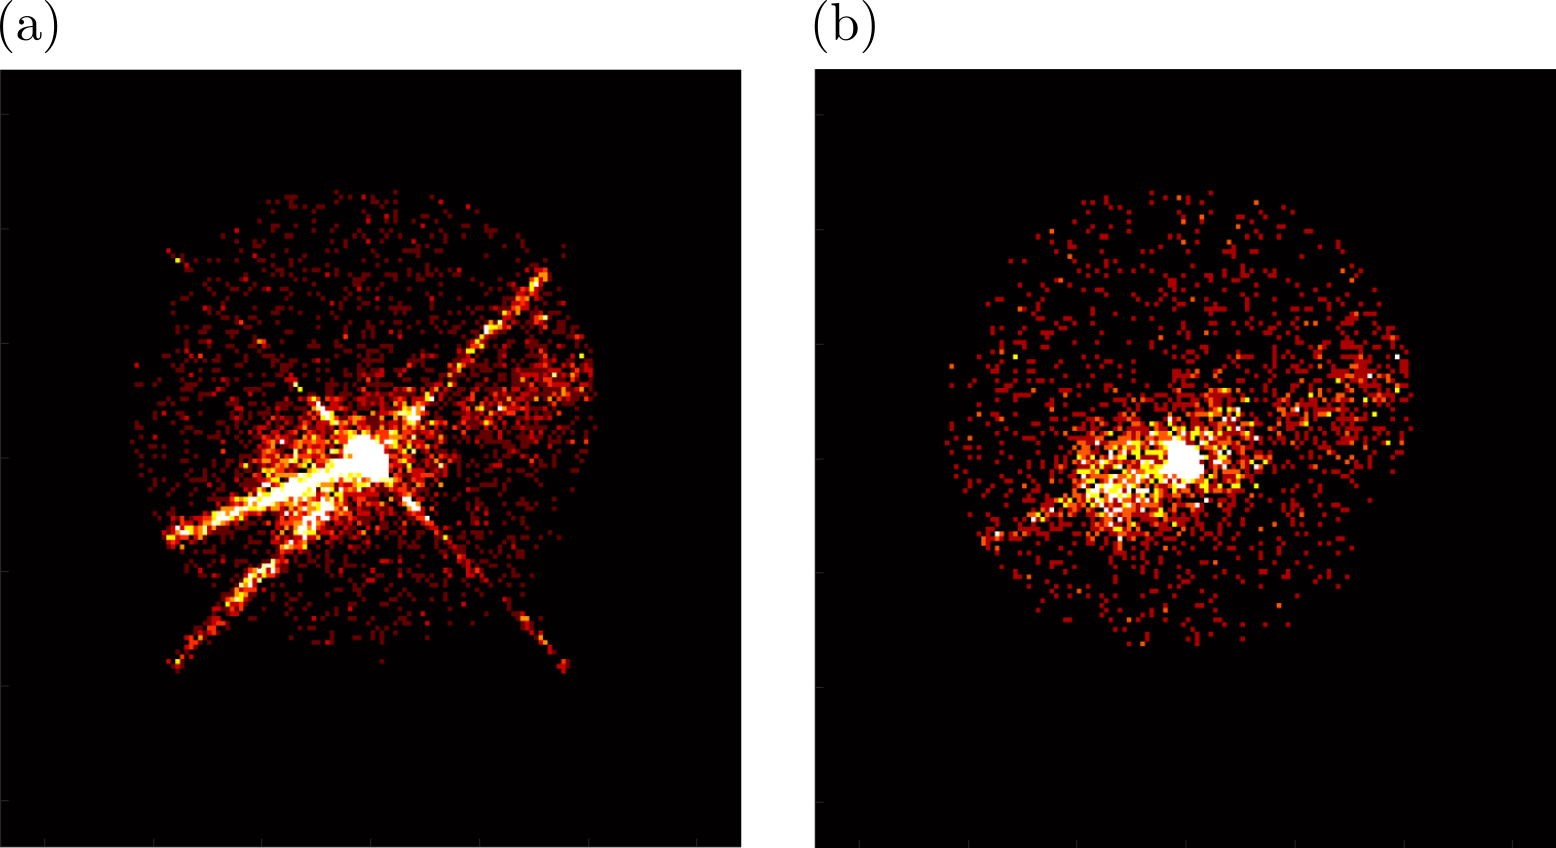
\includegraphics[width=\textwidth]{Fig/Chapter4/correction_saturation.png}
    \caption[Correction of software saturation]{Correction of software saturation. (a) Time integrated 2D MCP image, uncorrected, with the saturation cross as already shown in \ref{sec:saturation_effect}. (b) Same image where the region $|k_z| < 0.05 \ k_d$ has been removed. The saturation cross has disappeared.}
    \label{fig:saturation_correction}
\end{figure}



\subsection{Transverse integration}

\label{sec:transverse_integration}

Now that we know how to numerically obtain the 3D histogram of the $\gtwo$ function, we must discuss how to represent the data. One of the most natural and intelligible way to do so is to plot 1D cuts of the $\gtwo$ function along the three direction of space to properly visualize the 3D correlation peak located in $\delta \bm{k} = \bm{0}$. To extract a 1D cut along the $x$ direction for instance, we could simply take the line of voxels verifying $\delta k_y=\delta k_z =0$. However, this is often not sufficient to have a proper signal-to-noise ratio. We therefore rather average the values of several voxels lines associated to $\delta \bm{k}$ values verifying $\abs{\delta k_y, \delta k_z} \leq \Delta k_{\perp}$ as illustrated on Fig-\ref{fig:cube_integration}, where $\Delta k_{\perp}$ defines the transverse integration. Note that this procedure applies for both normal and anomalous correlation functions.

\begin{figure}
    \centering
    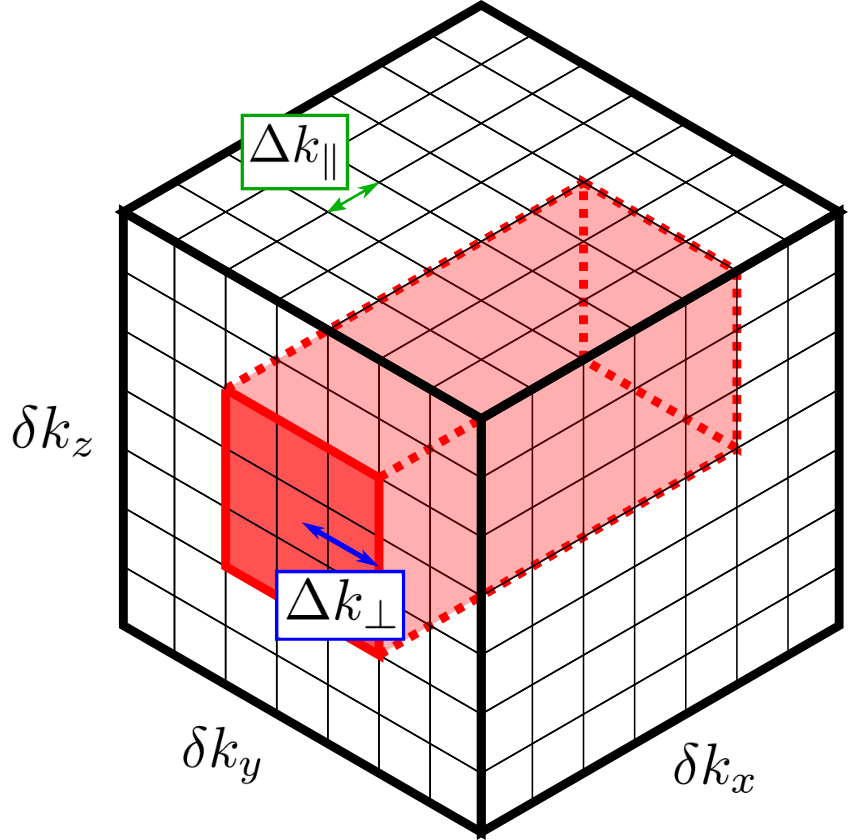
\includegraphics[width=0.45\textwidth]{Fig/Chapter4/cube_integration.png}
    \caption[Illustration of the transverse integration]{Illustration of the transverse integration. Every voxel contains the value of the $\gtwo$ function for a given value of $\delta \bm{k}=(\delta k_x, \delta k_y, \delta k_z$). The figure illustrates the procedure to take a 1D cut in the $x$ direction: we average over several pixel lines to increase the signal-to-noise ratio. This is the transverse integration $\Delta k_{\perp}$ as defined on the schematic.}
    \label{fig:cube_integration}
\end{figure}

We now write what is the signal that is plotted when this process is applied. The theoretical, normalized and integrated two-body correlation function is well modelled in first approximation by a 3D Gaussian function:

\begin{equation}
    \gtwo (\delta \bm{k}) = 1 + \eta_0 \prod_{i=x,y,z} \exp \left(\frac{-\delta k_i^2}{2 \sigma_i^2}\right)
    \label{eq:g2_theo}
\end{equation}

\noindent where we introduce $\eta_0$ the amplitude of the correlation peak and $\sigma_i$ the RMS width of the correlation peak in direction $i=x,y,z$. Importantly, we have assumed that the different correlation axis are separable. We re-write this equation to account for the transverse integration process, with the example of a cut along the $x$ direction:

\begin{equation}
    g^{(2)} \left(\delta k_{x}\right)=\frac{1}{\left(2 \Delta k_{\perp}\right)^{2}} \iint_{-\Delta k_{\perp}}^{\Delta k_{\perp}} \left( 1+ \eta_0 \prod_{i=x, y, z} \exp \left(\frac{-\delta k_{i}^{2}}{2 \sigma_i^{2}}\right) \mathrm{d} \delta k_y \mathrm{d} \delta k_z \right)
\end{equation}

\noindent This expression can be analytically evaluated and writes:

\begin{equation}
    g^{(2)} \left(\delta k_{x}\right)=1+\eta_0 \frac{2 \pi \sigma_y \sigma_z}{\left(2 \Delta k_{\perp}\right)^{2}} \exp \left(\frac{-\delta k_{x}^{2}}{2 \sigma_{z}^{2}}\right) \operatorname{erf}\left(\frac{\Delta k_{\perp}}{\sqrt{2} \sigma_{y}}\right) \operatorname{erf}\left(\frac{\Delta k_{\perp}}{\sqrt{2} \sigma_{z}}\right)
\end{equation}

Note that we have here neglected the small longitudinal integration induced by the size of the voxel, which is typically 3 times smaller than the RMS width of the correlation peaks in our experimental data. In addition, we assume that the correlation peaks are isotropic as the lattice potential and then the spatial size of the gas are isotropic, giving $\sigma_x=\sigma_y=\sigma_z=\sigma$. We thus see that when measuring any correlation peak amplitude with a Gaussian fit on a 1D cut of the $\gtwo$ function, we get a reduced amplitude $\eta$ that writes:

\begin{equation}
    \eta (\Delta k_{\perp})= \eta_{0} \times \frac{2 \pi \sigma^2}{(2\Delta k_{\perp})^2}\left[\rm{erf} \left(\frac{\Delta k_{\perp}}{\sqrt{2}\sigma} \right)\right]^2
    \label{eq:fit_integration}
\end{equation}

The idea is then to measure $\eta$ for several values of $\Delta k_{\perp}$ and fit the data with equation \ref{eq:fit_integration} with $\eta_0$ and $\sigma$ as free parameters. This is illustrated on Fig-\ref{fig:integration_kk} and Fig.-\ref{fig:eta_vs_int_kmk} for \kk and \kmk correlations respectively. For a single value of the transverse integration, $\eta$ is obtained by averaging the 3 amplitudes fitted on the 1D cuts along the 3 directions of space. The uncertainty on the parameters of the fit defines the error bars on the amplitude.

In addition, we have checked that the transverse integration process does not significantly change the width of the correlation peak as shown on the inset of Fig.-\ref{fig:eta_vs_int_kmk}. The extracted width is therefore the fitted width at the lowest transverse integration for which we get a satisfactory signal to noise ratio.

\begin{figure}
    \centering
    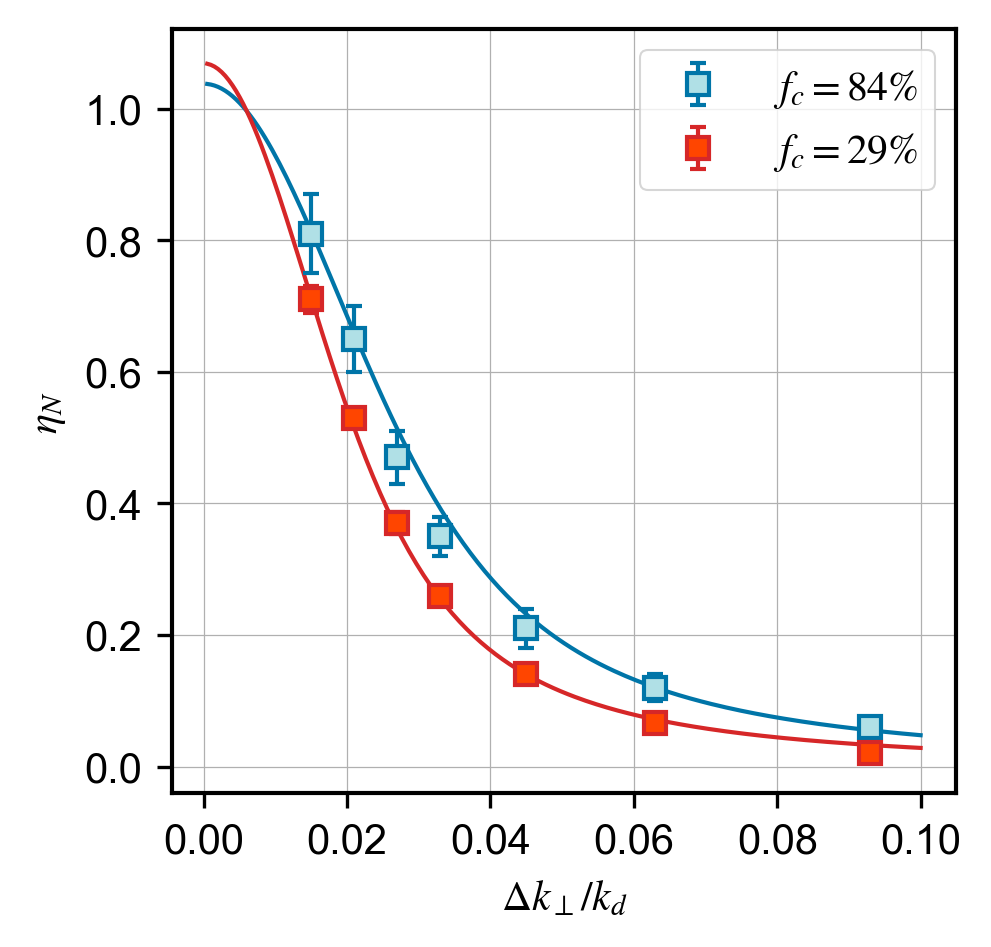
\includegraphics[width=0.65\textwidth]{Fig/Chapter4/eta_vs_int_kk.png}
    \caption[Fitted amplitude of the normal correlation peak $\eta_N$ as a function of the transverse integration $\Delta k_{\perp}$]{Fitted amplitude of the normal correlation peak $\eta_N$ as a function of the transverse integration $\Delta k_{\perp}$ for data sets with different condensed fraction. The data is fitted with model defined in equation \ref{eq:fit_integration} with $\eta_0$ and $\sigma$ as free parameters. This method allows us to extract the amplitude at zero transverse integration $\eta_{0,N}$.}
    \label{fig:integration_kk}
\end{figure}

\begin{figure}
    \centering
    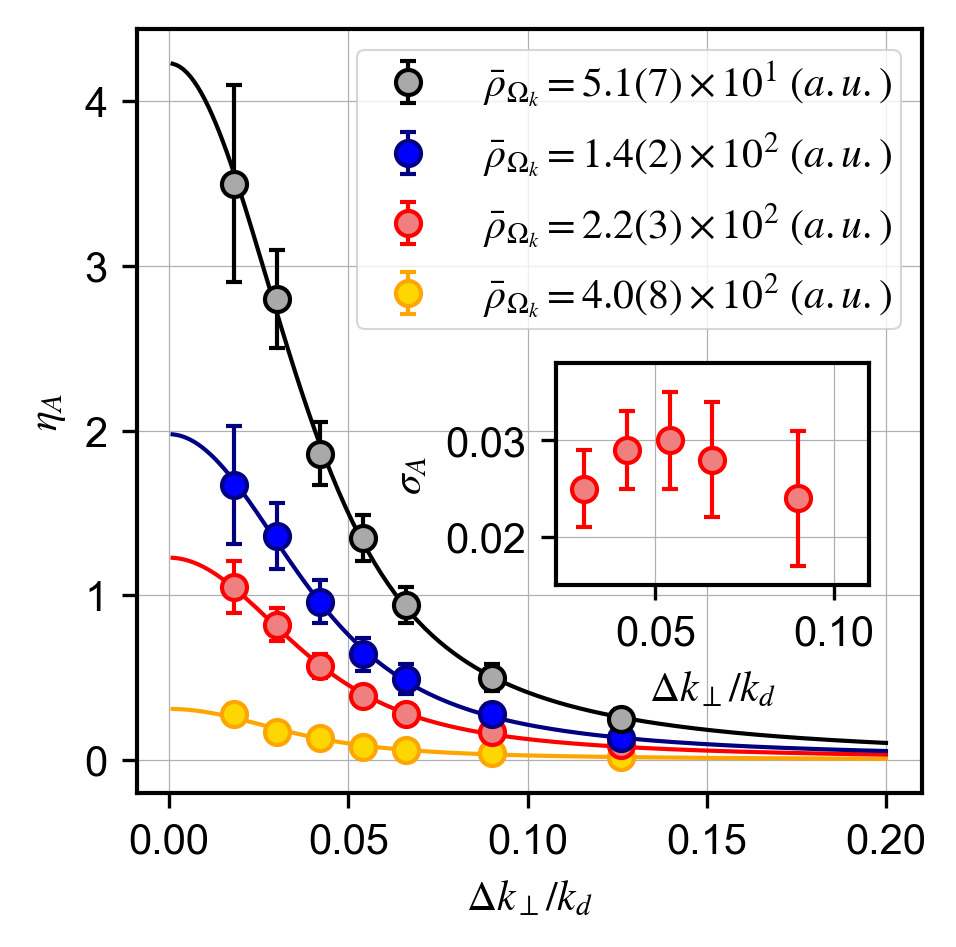
\includegraphics[width=0.65\textwidth]{Fig/Chapter4/eta_vs_int_kmk.png}
    \caption[Fitted amplitude of the anomalous correlation peak $\eta_A$ as a function of the transverse integration $\Delta k_{\perp}$]{Fitted amplitude of the anomalous correlation peak $\eta_A$ as a function of the transverse integration $\Delta k_{\perp}$ for data sets with various average densities $\rhob$ (see later). The inset represents the fitted width $\sigma_A$ as a function of the transverse integration $\Delta k_{\perp}$. No significant effect can be observed within the error bars.}
    \label{fig:eta_vs_int_kmk}
\end{figure}

\subsection{Benchmarking of the algorithm with two-body collision spheres}

\label{sec:benchmark_algo}

Before using the algorithm to look for \kmk pairing signal in the depletion of a weakly-interacting Bose gas, it was crucial to test it on a data set with a large number of \kmk pairs to certify that it was working properly. Luckily, we could re-use the data taken for measuring two-body collisions during the time-of flight described in Chapter \ref{sec:chapter_3}. Indeed, because of the elastic character of the collision, every atom on a collision sphere is correlated with a partner on the other side of the sphere, yielding \kmk correlations in the reference frame of the center of mass of the colliding BECs \cite{hodgman2017solving,perrin2007observation}. In addition to the 3D diffraction data that we already presented, we also took into data recorded with a single lattice beam to induce 1D diffraction and obtain only two collision spheres (see Fig.-\ref{fig:1D_spheres}). The advantage is that we have a large number of atoms in these collision spheres, making the analysis easier. 

\begin{figure}
    \centering
    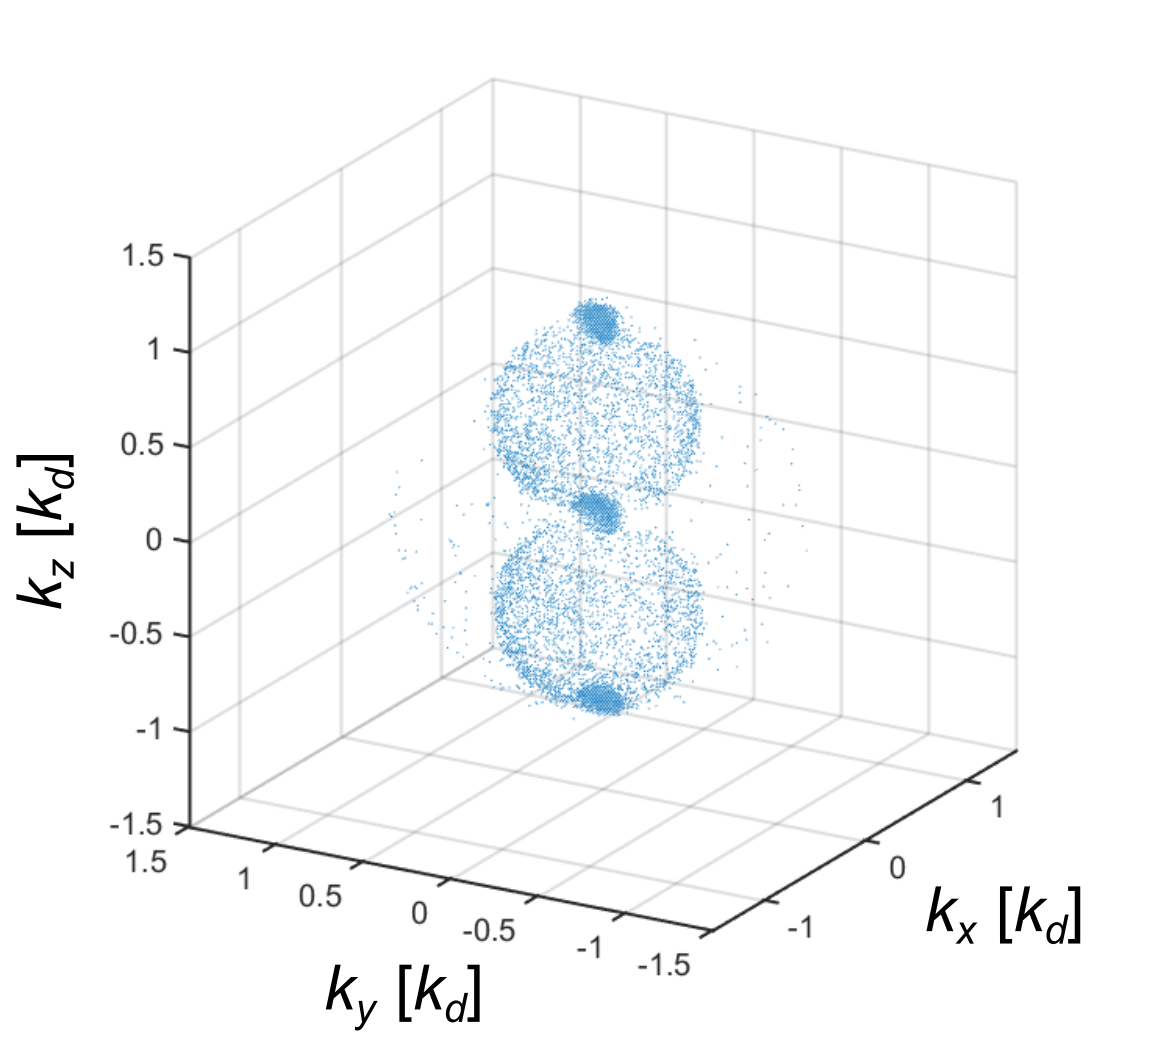
\includegraphics[width=0.7\textwidth]{Fig/Chapter4/1d_spheres.png}
    \caption[1D diffraction and associated collision spheres]{1D diffraction and associated collision spheres. Note that while the condensed peaks are shown here, they are removed before calculating the correlations.}
    \label{fig:1D_spheres}
\end{figure}

Contrary to the \kmk correlations of the quantum depletion, we de not expect a correlation peak at $\delta \bm{k}=\bm{0}$. If we consider for instance collisions between the 0th and 1st orders of diffraction along $z$, the overall momentum before and after the collision is $k_d \bm{z}$ ($\bm{z}$ is the unitary vector of the $z$ axis), so that the sum of the momenta of the two correlated atoms after the collision must be $k_d \bm{z}$. We thus expect a correlation peak for each sphere, one at $\delta k = (0,0,+1 \ k_d)$  and one at $\delta k = (0,0,-1 \ k_d)$.

We run the algorithm on the experimental data and obtain the results shown in Fig.-\ref{fig:kmk_kapitza}. We observe two correlation peaks at the expected locations! We can now extract the width and amplitude of the peaks with a Gaussian fit and see if they match with the results of \cite{tenart2020two} detailled in Chapter \ref{sec:chapter_3}. We find RMS widths of $\sigma_A=2.3(9) \times 10^{-2} \ k_d$ and $\sigma_A=2.7(8) \times 10^{-2} \ k_d$ for the spheres centered on $-k_d$ and $+k_d$ respectively, the error bars being given by the uncertainty on the fit coefficients. This is consistent with the measured widths of the scattering halos presented in \ref{sec:width_halos}, namely $\delta k_s = 2.1(9) \times 10^{-2}$ for $\NBEC=1.25 \times 10^5$ close to the total number of atoms used here. 
The prediction of the amplitude is rather straightforward in this configuration as we know that every atom on the sphere has a momentum correlated partner, allowing us to compare it to the experiment. To count the experimental number of detected pairs, we use the following procedure:


\begin{enumerate}
    \item The voxel size is increased to $\Delta k_{\parallel} = 0.25 \ k_d$ so that a single voxel contains the correlation peak entirely to count all true correlations.
    
    \item We count the number of coincidences $N_{\rm{numerator}}$ in the voxel centered on a correlation of the numerator histogram of equation \ref{Eq:g2_anomalous}. 
 
   
    \item  We count the number of coincidences $N_{\rm{denominator}}$ in the same voxel of the denominator of equation \ref{Eq:g2_anomalous} to evaluate the number of accidental coincidences. 
    
    
    \item As the numerator contains both true and accidental coincidences, we evaluate the number of true coincidences by subtracting the number of accidental coincidences and taking into account the normalization factor:
    \begin{equation}
          2N_{\rm{pairs}}=\Big(N_{\rm{numerator}} - N_{\rm{denominator}}\Big) \times \frac{\sum_i N_i^2}{(\sum_i N_i)^2}
    \end{equation}
    where the factor 2 is added as we define $N_{\rm{pairs}}$ as the number of pairs and we rather obtain the number of paired atoms with this formula.
  
\end{enumerate}

We find that the average number of detected pairs per run is $N_{\rm{pairs}}/N_{\rm{runs}}=6.25$. This number must be compared to the number of pairs that we expect from the number of atoms in the spheres that we evaluate using the following procedure:

\begin{itemize}
    \item Writing $N_{\rm{tot}}$ the total atom number in a given sphere, we know that we should detect $N_{\rm{tot}} \alpha_{\rm{MCP}}^2/2$ correlated pairs, where $\alpha_{\rm{MCP}}$ is the detection efficiency of the $\He$ detector. 
    \item The number of detected atoms in the considered sphere is simply $N_{\rm{tot}} \alpha_{\rm{MCP}}$. Multiplying this measured number by $\alpha_{\rm{MCP}}/2$, we thus obtain the expected number of correlated pairs.
\end{itemize}

We find that we expect to detect $8.5(5)$ pairs per run which is rather consistent with the number of detected pairs per run. The uncertainty is given by the uncertainty on the detection efficiency. Note that as this experiment was done before the implemention the two-photon Raman transfer scheme, the detection efficiency was lower than what was calibrated in Chapter \ref{sec:chapter_3} and was equal to $\alpha_{\rm{MCP}}=6.5(4) \%$.




\begin{figure}
    \centering
    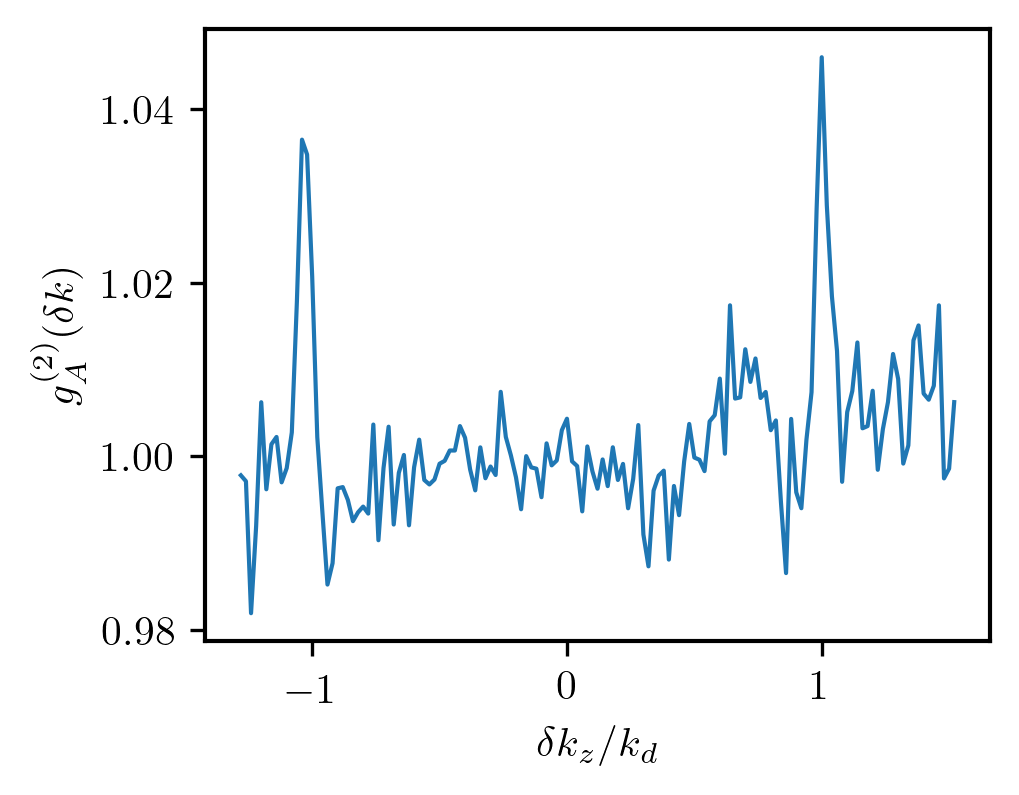
\includegraphics[width=0.7\textwidth]{Fig/Chapter4/kmk_kapitza.png}
    \caption[1D cut of the anomalous correlation function $\gtwo_A$ along the $z$ axis]{1D cut of the anomalous correlation function $\gtwo_A$ along the $z$ axis. We observe two correlation peaks, one for each correlation sphere. The longitudinal size of the voxels is $\Delta k_{\parallel}= 2 \times 10^{-2}$ and the transverse integration $\Delta k_{\perp}= 9 \times 10^{-2}$.}
    \label{fig:kmk_kapitza}
\end{figure}


\section{Observation of the pair correlation signal}

Now that we have determined the numerical procedure to extract the correlation signals from the raw data, we look to apply it on our experimental data. In this section, we will present the measured \kmk correlation signal of which we will try to understand the main features. Our goal is to first identify clear arguments linking this signal to the quantum depletion, before going into quantitative details that will be the subject of the next section.

\subsection{Accessing the BEC depletion}
\label{sec:accessing_depletion}

In order to detect \kmk pairs in the depletion, it is absolutely crucial to remove from the analysis all atoms belonging to the BEC and its diffracted copies as explained in Chapter \ref{sec:chapter_1} \ref{sec:ch1_separation}. For each recorded data set and before running the algorithm, we remove all atoms outside the volume $\Omega_k$ that we design to exclude momentum regions with condensed atoms as illustrated on Fig-\ref{fig:omega_k}. We set $\Omega_k$ to have a cubic symmetry that matches the symmetry of the momentum distribution in a cubic lattice. We remove all atoms with $|k_i| < k_{\rm{min}}$ and $|k_i| > k_{\rm{max}}$ where $k_i$ is the momentum projection along an axis $i=x,y,z$. We use $k_{\rm{min}}=0.15 \, k_d$, corresponding to $\sim 6$ times the RMS width of the BEC peaks, in order to ensure that all condensed atoms have been removed. The high limit is set to $k_{\rm{max}}=0.85 \, k_d$ to exclude higher order peaks and is slightly smaller than the momentum range probed by the MCP. In terms of healing length, this corresponds to $0.85 \leq | k | \xi \leq 1.15$, \ie the region where the phononic character of the Bogoliubov quasi-particles is negligible and thus where finite temperature excitations do not contribute to the anomalous correlations. 

\begin{figure}
    \centering
    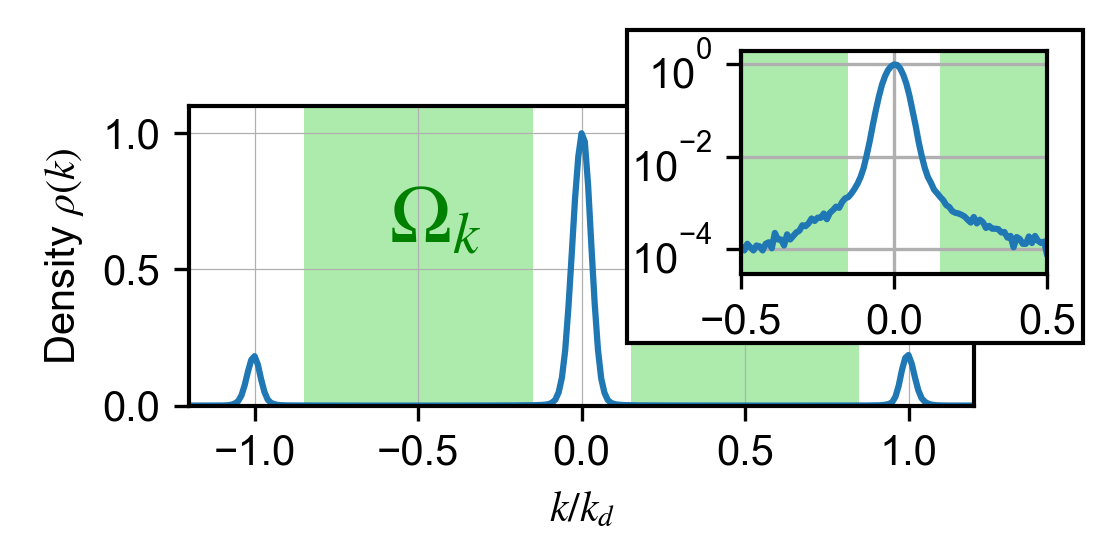
\includegraphics[width=0.8\textwidth]{Fig/Chapter4/densite.png}
    \caption[1D cut of the momentum density illustrating the integration volume $\Omega_k$]{1D cut of the momentum density illustrating the integration volume $\Omega_k$. The central peak corresponds to the BEC and the lateral peaks at $\pm \ k_d$ to diffraction peaks induced by the presence of the optical lattice. The green area shows the volume $\Omega_k$ containing the depleted atoms selected for the correlation measurement. While barely visible in linear scale, they can be seen in the log scale plot shown in inset.}
    \label{fig:omega_k}
\end{figure}




\subsection{First characterization of the pair correlation signal}

\label{sec:post_selec}

As we have checked that the algorithm is working properly, we now look to observe the \kmk pairs of the quantum depletion.



\begin{figure}[]
    \centering
    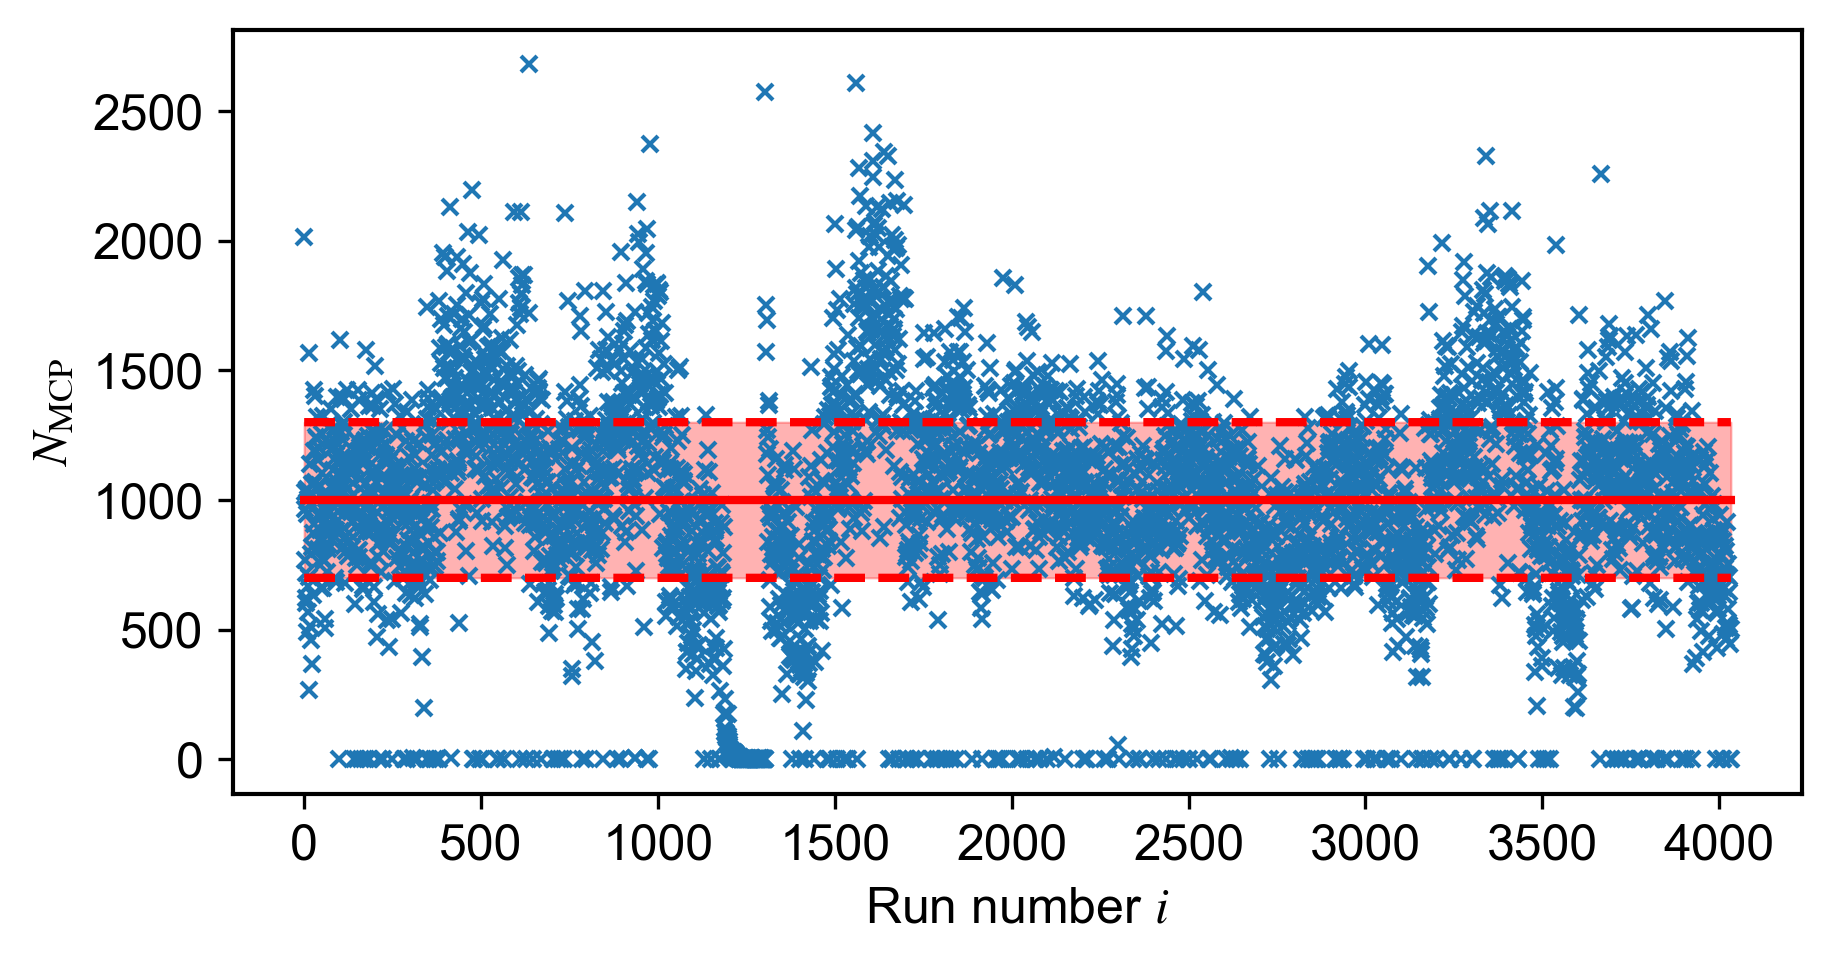
\includegraphics[width=0.95\textwidth]{Fig/Chapter4/n_fluctuations.png}
    \caption[Number of detected atoms $N_{\mathrm{MCP}}$ for each experimental runs of a data set]{Number of detected atoms $N_{\mathrm{MCP}}$ for each experimental runs of a data set. The full red line represents the target detected atom number. The red shaded area between the dashed lines illustrate the allowed fluctuations of the detected atom number. All runs outside of the red area are rejected.}
    \label{fig:n_fluctuations}
\end{figure}

We prepare a BEC with a target number of $\NBEC=5 \times 10^3$ atoms in an optical lattice of amplitude $V=7.75 \ E_r$. With this lattice amplitude, we are in the superfluid regime of the phase diagram in which we expect the \kmk correlations: we measure a condensed fraction of $84 \%$ corresponding to a depletion level for which the Bogoliubov theory is expected to hold (see Supp. Mat. of \cite{lopes2017}). In order to have sufficient statistics, we repeat the experiment $\sim 4,000$ times. In practice, we cannot prepare BECs with the exact same number of atoms at each shot. Note that the atom number fluctuations of large BECs of $\NBEC=5 \times 10^5$ atoms are below $10 \%$ but when we attempt to work with only $\NBEC=5 \times 10^3$ atoms, shot-to-shot fluctuations are much larger. 

We then need to post-select the data and remove runs with a detected atom number falling too far from the target number. This is one of the strengths of our experiment: as each atom has the same probability of being detected, we can select shots with the good total atom number a posteriori with a precision unattainable with optical imaging measuring densities. This must however be mitigated by the fact saturation effects reduces the number of detected atoms in a way that can be hard to predict precisely. We allow for $30 \%$ fluctuations around the target number (see Fig.-\ref{fig:n_fluctuations}) and end up conserving around $\sim 2,000$ runs on which we run the algorithm.

\begin{figure}[ht!]
    \centering
    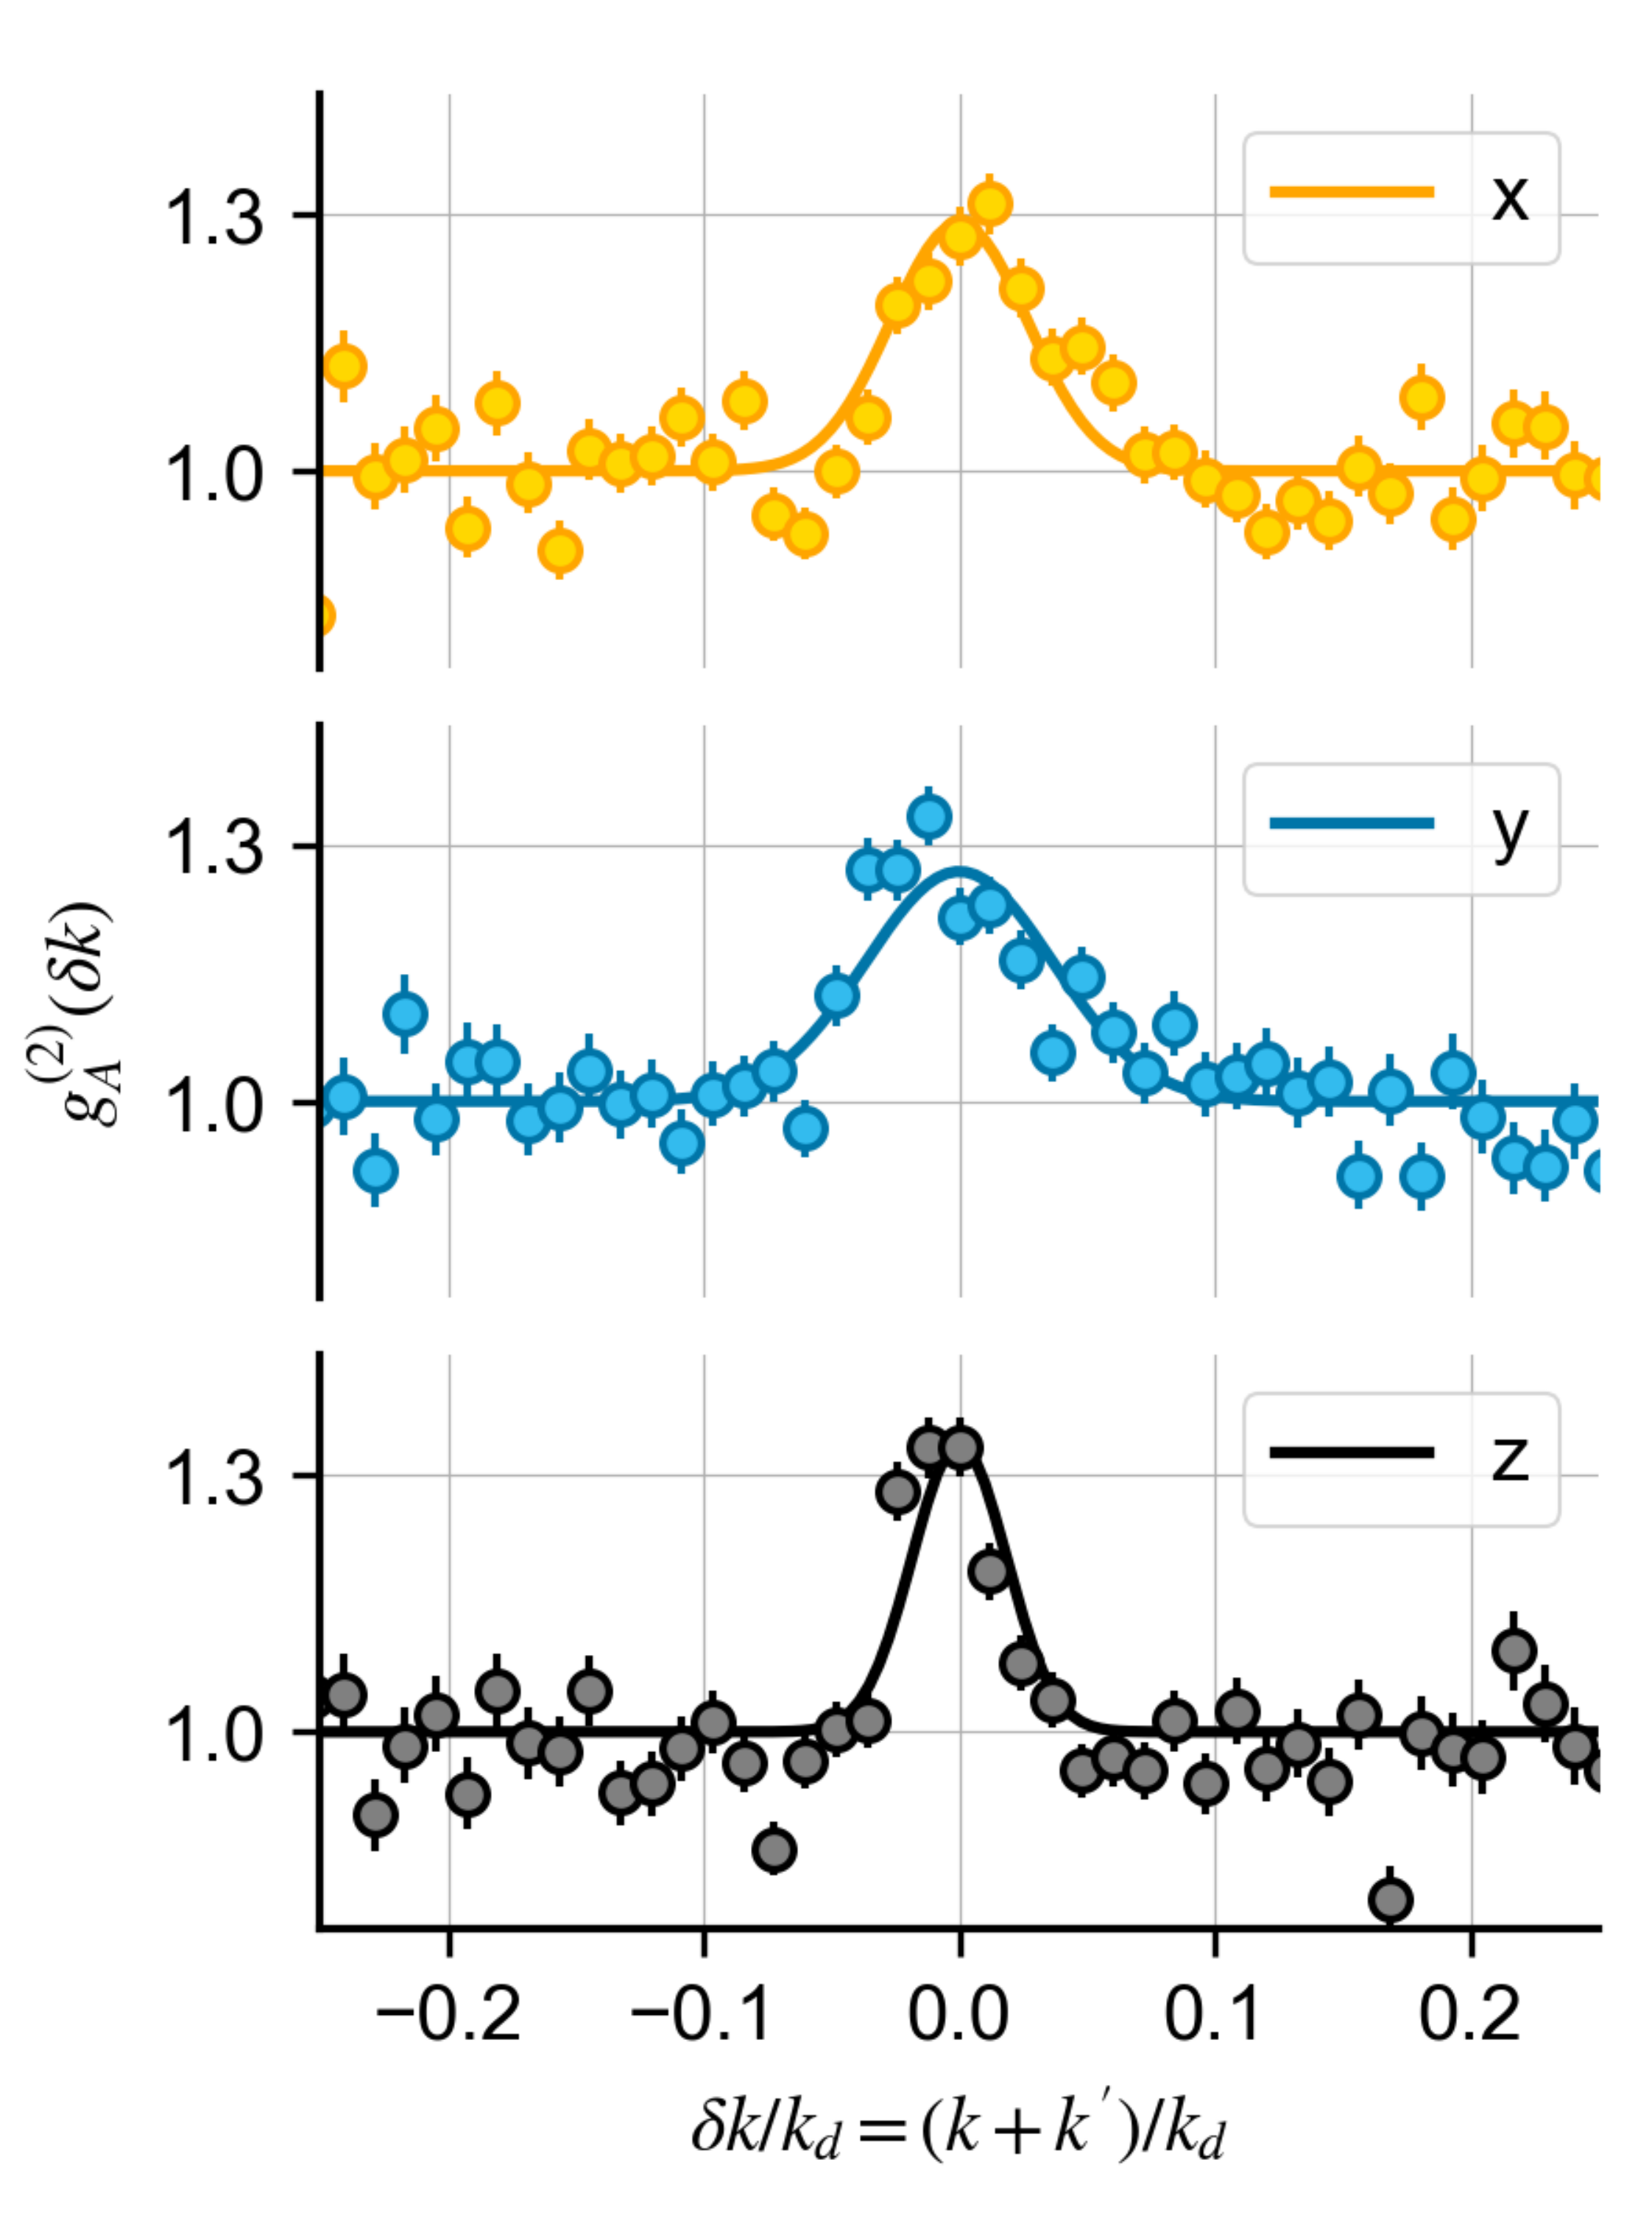
\includegraphics[width=0.65\textwidth]{Fig/Chapter4/correlations_kmk_errorbars.png}
    \caption[1D cuts through the anomalous correlation function $g_{A}^{(2)}$ along the axis of the 3D optical lattice]{1D cuts through the anomalous correlation function $g_{A}^{(2)}$ along the axis of the 3D optical lattice. The transverse integration is $\Delta k_{\perp}=3 \times 10^{-2} \ k_d$ and the longitudinal voxel size is $\Delta k_{\parallel}=1.2 \times 10^{-2} \ k_d$. The data is fitted by Gaussian functions (solid lines). The nice correlation peaks signal the presence of \kmk pairs. The error bars are obtained from the inverse square root of the number of counts in the voxels.}
    \label{fig:kmk_signal}
\end{figure}

We have plotted on Fig-\ref{fig:kmk_signal} 1D cuts through the calculated $g_{A}^{(2)}$ function on which we see clear correlation peaks standing out from the noise! This is the kind of signal we were aiming to obtain and constitutes the central result of this thesis. Before analyzing the features of this correlation signal in more details, we conduct a first series of experimental checks. First, we extend the range of $\delta \bm{k}$ on which we plot the $g_{A}^{(2)}$ function to find correlation peaks at $\delta k = \pm k_d$ as shown on Fig.-\ref{fig:periodicity}. This is something that we expected from Bloch theorem (see \ref{sec:BH_model}) as the lattice is a periodic potential.

\begin{figure}
    \centering
    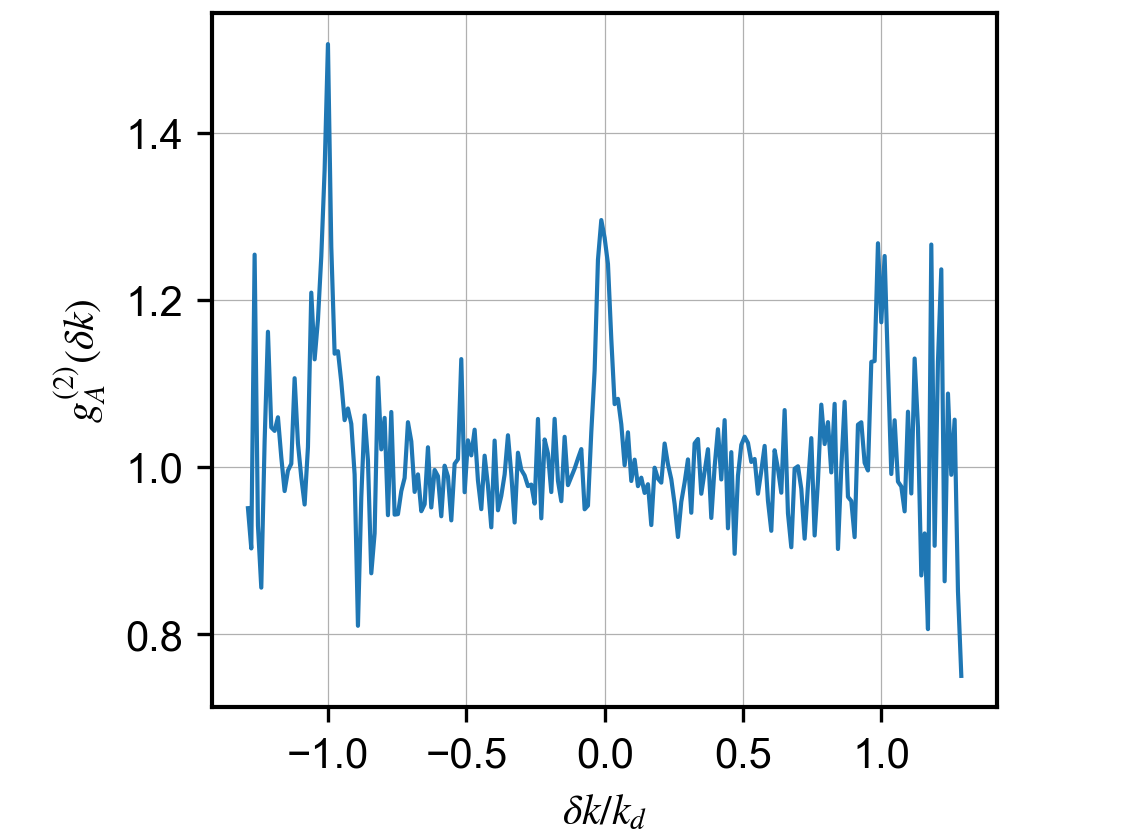
\includegraphics[width=0.7\textwidth]{Fig/Chapter4/periodicity.png}
    \caption[1D cut of the anomalous correlation function $\gtwo_A$ illustrating its periodicity]{1D cut of the anomalous correlation function $\gtwo_A$. Because of the lattice periodic potential, we observe additional correlation peaks at $\pm k_d$.}
    \label{fig:periodicity}
\end{figure}

Furthermore, we check that there are no correlations in the coherent BEC state. We do so by selecting atoms with $|k_i|<0.04 \ k_d$ with $i=x,y,z$. We show on Fig.-\ref{fig:BEC_correlations} the calculated normal and anomalous correlation functions for the mode of the BEC. As expected, both correlation functions are flat, except for a small modulation of the order of $1 \%$ that is an artifact of the normalization procedure caused by shot-to-shot fluctuations of the width of the BEC (see \cite{cayla_these}).

\begin{figure}
    \centering
    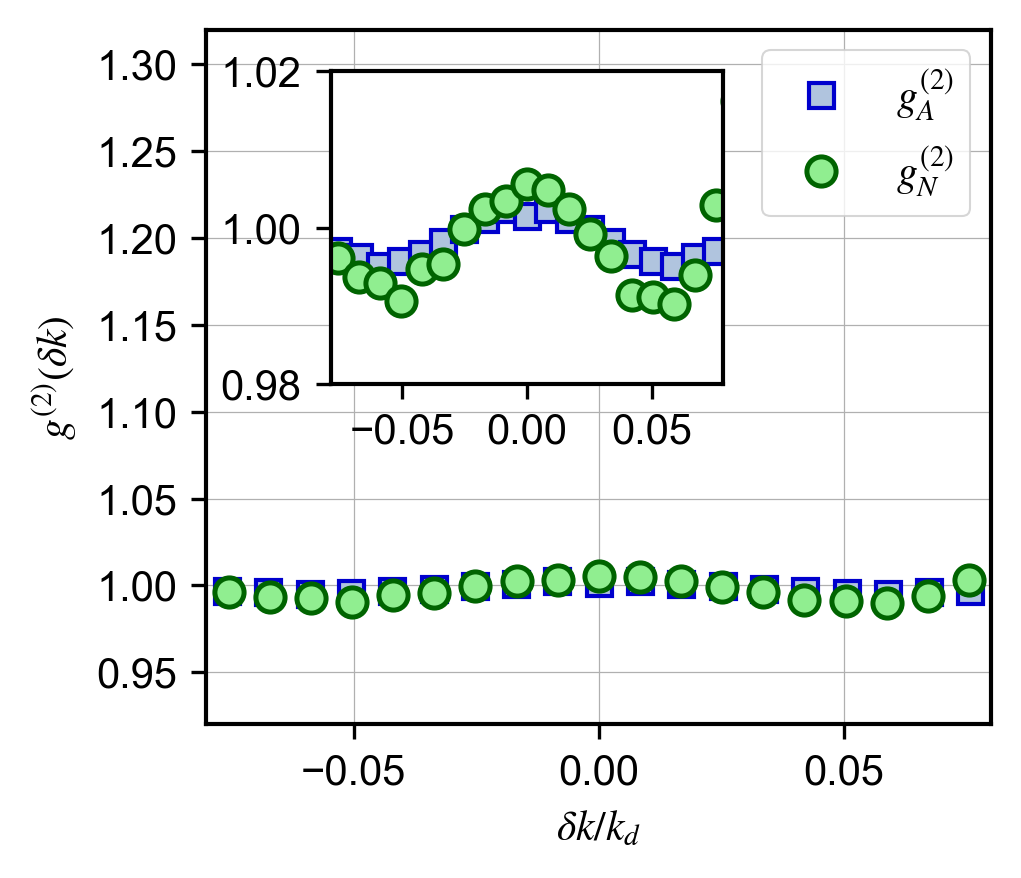
\includegraphics[width=0.65\textwidth]{Fig/Chapter4/correlations_BEC.png}
    \caption[Normal and anomalous correlation functions in the BEC]{Normal and anomalous correlation functions in the BEC. The correlation functions are flat, except for a small-amplitude modulation that is due to normalisation issues induced by shot-to-shot fluctuations of the BEC width in momentum-space.}
    \label{fig:BEC_correlations}
\end{figure}

Now that we have observed an anomalous correlation signal, we must ask whether its origin is indeed the one we expect, namely \kmk pairing in the quantum depletion as a result of the interplay between interactions and quantum fluctuations. For starters, one of the key specificity of the \kmk pairs of the quantum depletion is that they exist in an \textbf{at-equilibrium} system. This is in strong contrast with \textbf{out-of-equilibrium} configurations where non linearities efficiently drive resonant processes. In these cases, both momentum and energy are conserved. In fact, \kmk pairing in such out-of-equilibrium systems has already been observed on various experimental platforms such as:

\begin{itemize}
    \item Parametric down conversion in quantum optics \cite{burnham1970}.
    \item Dissociation of diatomic molecules in atomic physics \cite{greiner2005}.
    \item Elastic collisions in high energy physics \cite{arnison1982} or with ultracold atoms \cite{perrin2007observation} as we have seen earlier (see Fig.-\ref{fig:kmk_kapitza}).
\end{itemize}

A main difference with the \kmk correlation signal obtained in the collision spheres is that we observe here a peak located at $\delta \bm{k} = \bm{0}$. This signals that the total momentum of the atom pair is $\bm{0}$. As our system consists of an at-rest BEC, the pairing process could not have resulted from an out-of-equilibrium effect. We remind here an important point of \ref{sec:pairing_mechanism}, which is that if we isolate a single collision, we find that the energy is not conserved as the two colliding atoms acquire momenta $\bm{k}$ and $-\bm{k}$ meaning that the total kinetic energy is $2 (\hbar^2 k^2/2m) \neq 0$. This shows that this effect cannot be explained classically because of the origin of the pairs, namely the quantum fluctuations. The pairs cannot be isolated as they form a single quantum state with the BEC, the many-body ground-state. This point constitutes the novelty of our experimental observation.

While these first observations seems to point towards the fact that we are indeed seeing the \kmk pairing of the quantum depletion, we look to further characterize the correlation signal and determine whether our observations are consistent with the results of the Bogoliubov theory to prove this point. To this end, we will first study the effect of temperature that is supposed to destroy the \kmk correlation signal linked to $T=0$ quantum coherences, as explained in Chapter \ref{sec:chapter_1} \ref{sec:ch1_temperature}.





\subsection{Effect of temperature}

\label{sec:kmk_temperature}

The temperature can be increased in a rather simple manner by holding the atoms at the final amplitude of the lattice for a longer duration, the gas being continuously heated over time (attributed to imperfections such as spontaneous emission or mechanical vibrations). We repeat the experiment with a holding time of $500 \ \rm{ms}$ corresponding to hundreds of tunneling times $225 \times h/J$. The increase in temperature can be seen by looking at the momentum density profile as shown in the panel (b) of Fig-\ref{fig:kmk_temperature}: the thermal depletion has increased, increasing the momentum density in the depletion region by a factor $\sim 4$. Note however that we did not increase the temperature too much to keep a significant condensed fraction of the order of $f_c = 29 \%$ (in the absence of BEC there is no quantum depletion). As the thermally depleted atoms show no \kmk correlations, only the denominator of equation \ref{Eq:g2_anomalous} increases as both $\rho(\bm{k})$ and $\rho(-\bm{k})$ increases each by a factor 4, thus reducing the amplitude of the anomalous correlation function by at least a factor 16, bringing it under the experimental noise as we see on Fig-\ref{fig:kmk_temperature} panel (a). Note that this reduction factor could in fact be even larger as the condensed fraction is small, meaning that the Bogoliubov approximation should not hold anymore. 

We also repeated the experiment for an intermediate temperature obtained with a holding time of $200 \ \rm{ms}$ corresponding to $90 \times h/J$ tunneling time. The condensed fraction is then $f_c=55 \%$ and we observe a peak of intermediate amplitude as shown on Fig-\ref{fig:kmk_3_temp}.

\begin{figure}
    \centering
    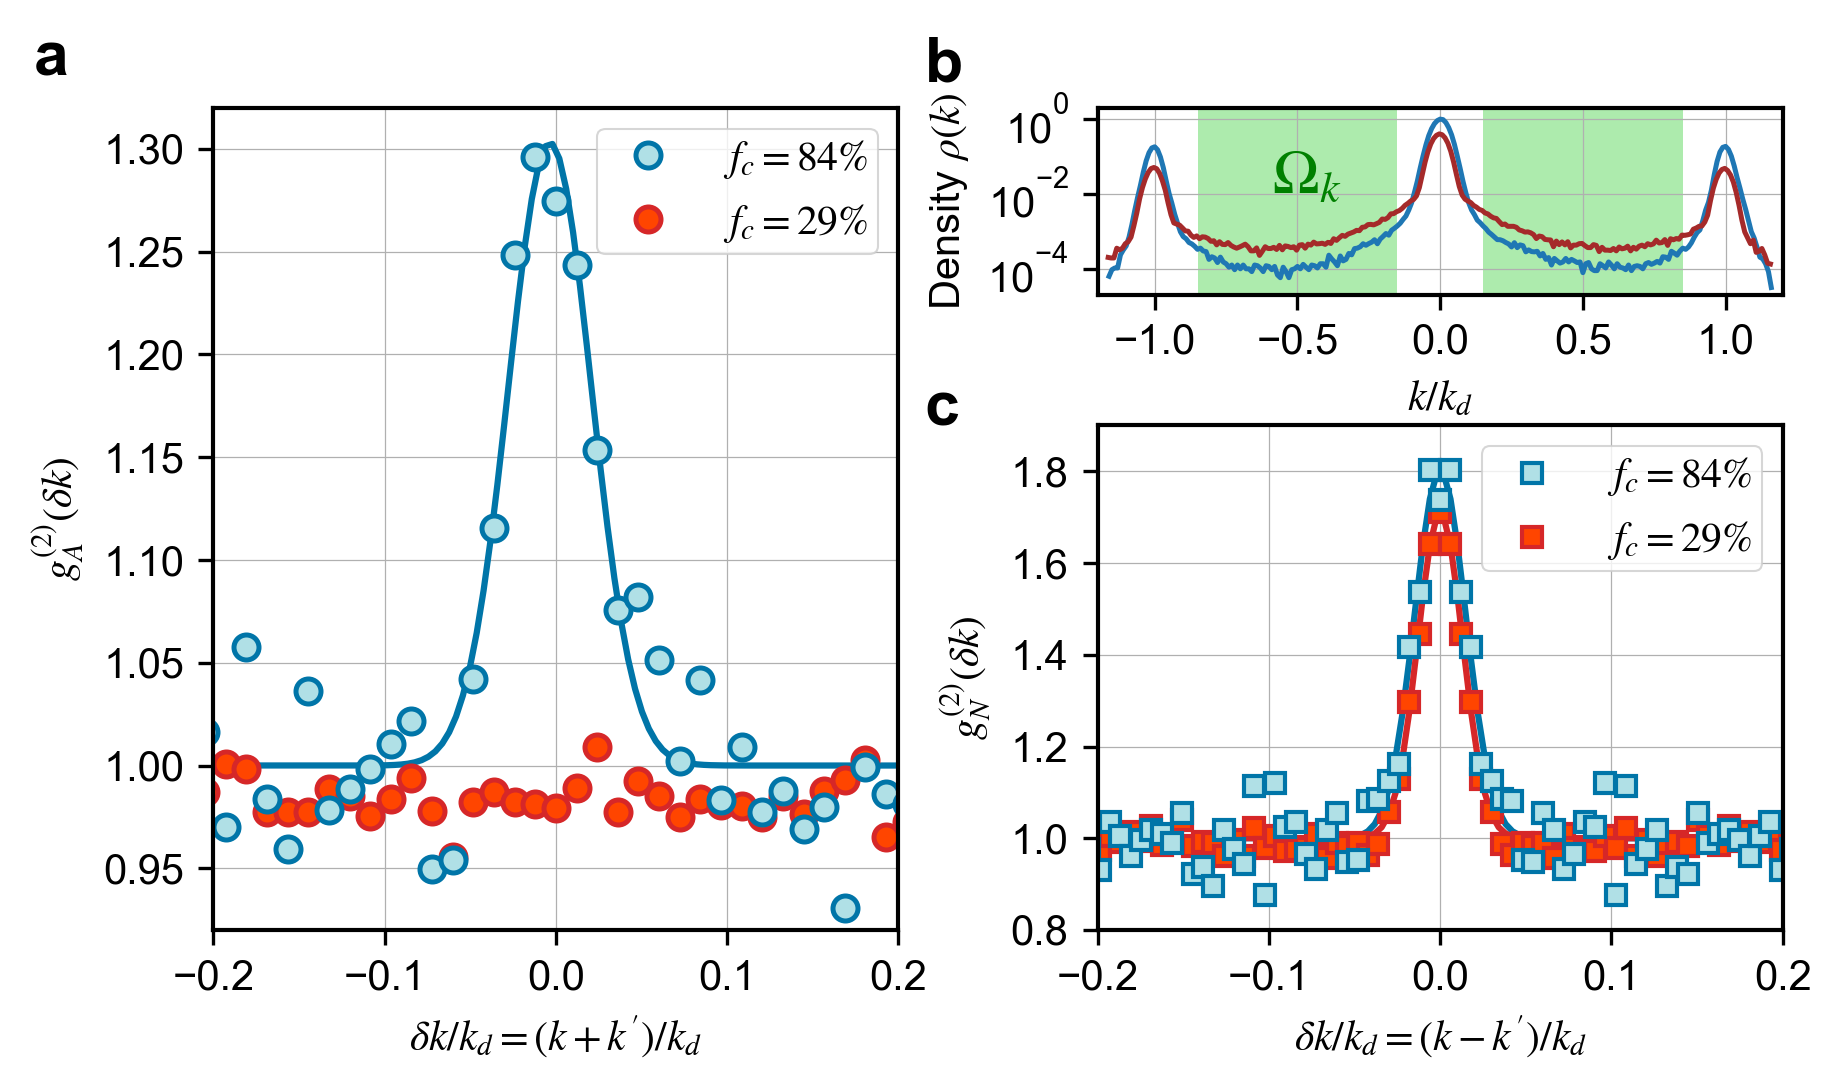
\includegraphics[width=\textwidth]{Fig/Chapter4/kmk_temperature.png}
    \caption[Atom-atom correlations in weakly-interacting BECs at two different temperatures]{Atom-atom correlations in weakly-interacting BECs at two different temperatures. The data for the low-temperature BEC ($f_{c}=84\%$), {\it resp.} for the heated BEC ($f_{c}=29\%$), are depicted in blue, {\it resp.} in red. 
    {(a)} Anomalous correlations $g_{A}^{(2)}(\delta k)$ at opposite momenta. The ${\bm k}$/$-{\bm k}$ peak disappears as the temperature increases.
    {(b)} 1D cut of the density $\rho(k)$ in semilog scale. The depletion density increases with temperature.
    {(c)} Normal correlations $g_{N}^{(2)}(\delta k)$ for the same datasets and $\Omega_k$. The peak amplitude shows no significant change as the temperature increases. Note that the transverse integration $\Delta k_{\perp}=1.5 \times 10^{-2} \, k_d$ used here reduces the amplitude of the peaks.}
    \label{fig:kmk_temperature}
\end{figure}

We thus observe that the \kmk correlation signal is extremely sensitive to temperature, hinting to the fact that it is related to a $T=0$ ground-state effect. It is also quite illuminating to compare the \kmk correlations to the bosonic bunching \kk correlations. As explained in Chapter \ref{sec:chapter_1}, the bosonic bunching effect is the consequence of chaotic statistics of bosons, a property shared by the thermal and quantum depletion. Therefore, changing the temperature and thus the balance between thermal and quantum depletion should have no effect on bosonic bunching. This is what we observe experimentally as shown on Fig-\ref{fig:kmk_temperature} panel (c).

In conclusion, we have on the same experimental data two very different behaviours with temperature that illustrate nicely the natures of the correlation signals. On the one hand, \kk correlations unaffected by temperature, reveal the chaotic statistics of the system. On the other hand, \kmk correlations reveal the quantum coherences in the many-body equilibrium state. These observations constitutes a rather convincing argument that we are indeed observing a \kmk correlation signal caused by the quantum depletion and not some other effect that we could have overlooked.

\begin{figure}
    \centering
    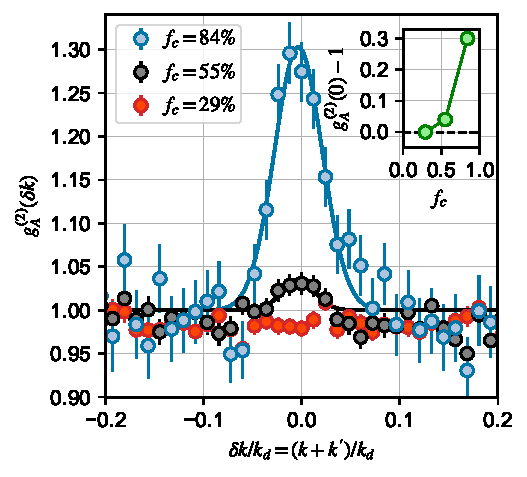
\includegraphics{Fig/Chapter4/kmk_3_temp_errorbars.pdf}
    \caption[Anomalous correlation function for data sets with different temperatures and condensed fractions]{Anomalous correlation function for data sets with different temperatures and condensed fractions. The amplitude of the $\bm{k}$/$-\bm{k}$ correlation signal is progressively lost as the temperature rises and the condensed fraction diminishes. Inset: amplitude of the correlation peak $g^{(2}_{A}({\bm 0})$ as a function of the condensed fraction $f_c$.}
    \label{fig:kmk_3_temp}
\end{figure}

In the following, we study in quantitative details these correlation signals. 


% To start on this topic, the attentive reader would have noticed than even though we expect perfect bosonic bunching $\gtwo_N (\bm{0})=2$, we rather observe $\gtwo_N (\bm{0}) \simeq 1.8$. This is due to transverse integration effects of the 3D $\gtwo$ function that need to be accounted for to extract the proper information from the amplitude of the correlation peaks.

\section{Study of the width of the correlation peaks}

\label{ref:exp_width_corr}

In a first stage, we study the width of the correlation peak, a quantity that actually contains meaningful information about the many-body equilibrium state. The key aspect is the same used by Hanbury Brown and Twiss in their seminal paper to measure the size of Sirius through the measurement of the second order correlation function in far-field, namely the width of the correlation peak is inversely proportional to the spatial size of the source. 

%This argument validates our previous assumption that the correlation peak is isotropic, as the lattice trapping potential is isotropic so that the spatial size of the BEC is the same in the three directions of space.

This subject has been discussed in \ref{sec:width_correlation_theo} in light of the results of the theoretical work \cite{butera2020}. We remind that as the anomalous correlations are exclusively caused by quantum depleted atoms whose spatial extent is the one of the BEC, the width of the anomalous correlation peak $\sigma_A$ is inversely proportional to the size of the BEC $L_{\rm{BEC}}$. On the other hand, the normal correlations are caused by quantum depleted atoms but also thermally depleted atoms whose spatial size extends beyond the BEC because of the increased kinetic energy. This tells us that the width of the normal correlations peak $\sigma_N$ should be smaller than that for anomalous correlations.

\begin{figure}
    \centering
    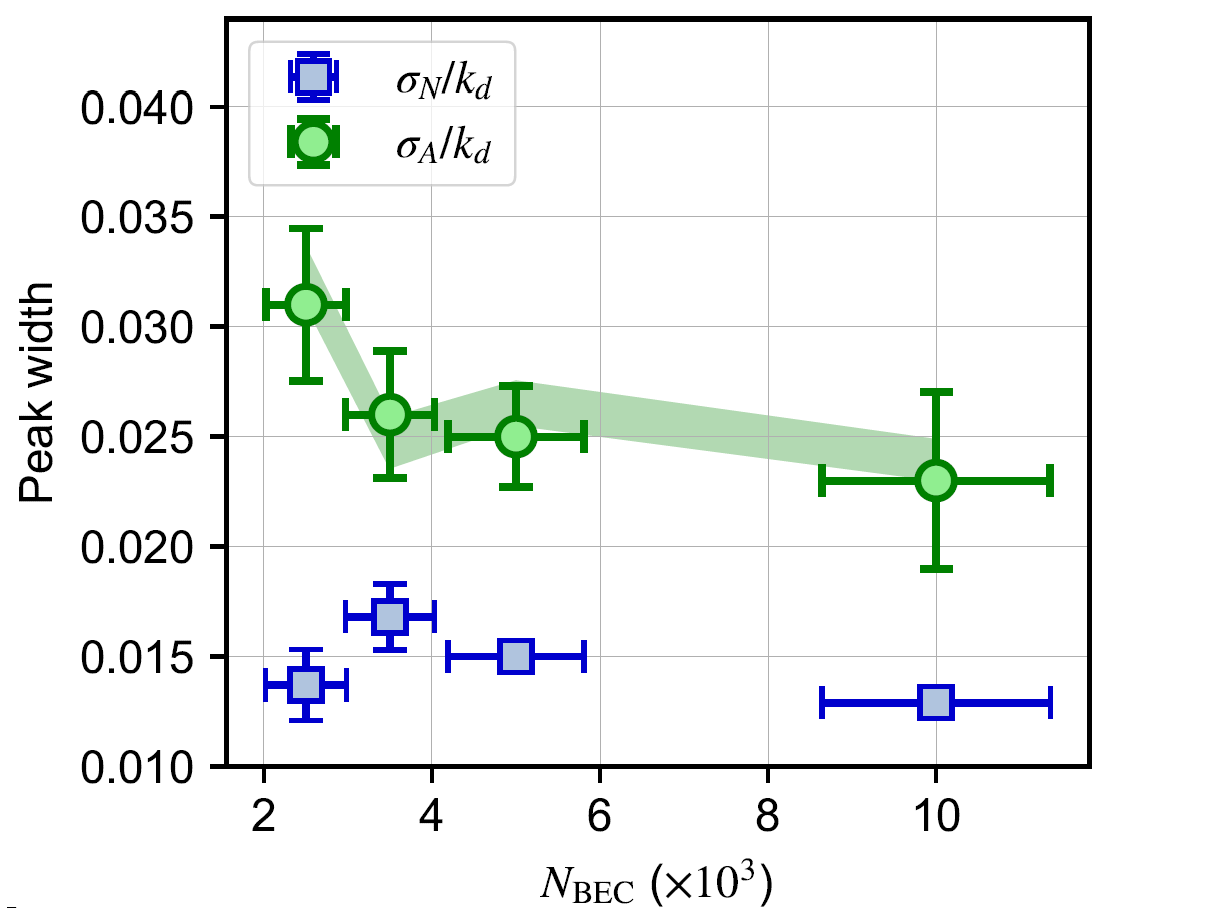
\includegraphics[width=0.65\textwidth]{Fig/Chapter4/widths.png}
    \caption[RMS widths of the anomalous and normal correlation peaks]{RMS widths of the anomalous (green) and normal (blue) correlation peaks. As expected from Bogoliubov theory, we get $\sigma_A > \sigma_N$ for each data set. The green area represents an estimation from the BEC width $\sigma_{\rm{BEC}}$ (see main text).}
    \label{fig:width}
\end{figure}

We plot on Fig.-\ref{fig:width} the experimental correlation peaks widths for different total atom numbers. The horizontal error bars correspond to the standard deviation of the total atom number, while the vertical error bars correspond to the standard deviation of the mean over the three directions of the momentum-space. With this first analysis, we observe that for all atom numbers, $\sigma_A > \sigma_N$. In addition, one would expect to see both widths decrease with the total atom number as the size of the system grows with $\NBEC$. This is more or less what the experimental data suggests but the error bar are too large to make a definite statement on this point. Note that in the Thomas-Fermi regime, the size of the BEC changes slowly with the total atom number $L_{\rm{BEC}} \propto \NBEC^{1/5}$, translating in a change of $\sim 30\%$ of the width of the correlation peaks from the data with $N=2.5 \times 10^3$ to $N=10 \times 10^3$ that is hard to resolve within our error bars.

We now look at the quantitative value of $\sigma_A$ that can be numerically evaluated. The calculations have been performed by S. Butera and I. Carusotto from the BEC center in Trento, Italy, with the Bogoliubov theory for a trapped 1D system \cite{butera2020}. They evaluate $\sigma_{A,\rm{theo}} = 0.94 \sigma_{\rm{BEC}}$, with $\sigma_{\rm{BEC}}$ the RMS width in momentum-space of the condensate. This relation is not modified in presence of a lattice as the size $L_{\rm{BEC}}$ does not change when the ratio $\mu/\hbar \omega$ is fixed. This is explained by the equality $m \omega^2 = m^* \omega^* ^2$ with $m^*$ the effective mass in the lattice and $\omega^*$ the corresponding effective frequency as defined in \ref{sec:rescaled_interaction}.

We can therefore measure $\sigma_{\rm{BEC}}$ to exploit this result. To do so, we need to account for deviations induced by the saturation of the detector. Indeed, the BEC is very dense resulting in a high flux of atoms saturating the detector. If we plot 1D cuts of the momentum density, the BEC momentum profile is then flattened at the top and fitting with a Gaussian function over-evaluates the momentum width of the condensate. To circumvent this issue, we adapt the parameters of the Raman transfer (see \ref{sec:raman}) to reduce drastically the flux of detected atoms and avoid saturating the detector to ensure proper fitting.

\subsubsection{Center-of-mass fluctuations}

During our first analysis, we noticed that the anomalous correlation peak was larger than that of the BEC, contrary to what we would have expected. We also noticed that the momentum width of the BEC was larger than what we obtained applying the Gutzwiller ansatz with our calibrated atom numbers. We attribute this to an imperfection in our experiment, the shot-to-shot fluctuations of the center-of-mass of the atomic distribution. When averaging over many experimental runs, these fluctuations enlarges artificially the measured width of the BEC, as well as the width of the anomalous correlation peak. These fluctuations can nevertheless be characterized by comparing the experimental momentum width of the BEC to the one predicted by the Gutzwiller variational approach.

When accounting for center-of-mass fluctuations, the measured momentum density results from the convolution with the distribution of center-of-mass displacements and has a RMS width:

\begin{equation}
    \sigma_{\rm{BEC}}=\sqrt{\sigma_{\rm{BEC},0}^2+\Delta k_{\rm{com}}^2}
\end{equation}

\noindent where $\sigma_{\rm{BEC},0}$ is the ``true'' BEC momentum width with $\sigma_{\rm{BEC},0} \propto 1/L_{\rm{BEC}}$. For instance, the Gutzwiller variational approach gives  $\sigma_{\rm{BEC},0} \simeq 1.7 \times 10^{-2} \ k_d$ for a total atom number $\NBEC = 5 \times 10^5$ and we measure $\sigma_{\rm BEC} = 2.00(4) \times 10^{-2} \ k_d$. From this we deduce $\Delta k_{\rm{com}}=1.05(2) \times 10^{-2} \ k_d$. Note that such fluctuations are small, corresponding to $1\%$ of the distance between the diffraction peaks. We repeat the procedure to evaluate $\Delta k_{\rm{com}}$ for all of the data sets of Fig.-\ref{fig:width}.

For a \kmk pair of atoms, a center-of-mass displacement ${\rm{d}} \bm{k}$ induces a momentum difference $\delta \bm{k}=2 {\rm{d}} \bm{k}$. The effect of the fluctuations are thus twice larger for the width of the anomalous correlations peak than for the BEC momentum width:

\begin{equation}
    \sigma_A = \sqrt{\sigma_{A,0}^2+4\Delta k_{\rm{com}}^2}
\end{equation}

\noindent Combining this with the numerical evaluation and the measured values of $\Delta k_{\rm{com}}$, we obtain a corrected estimate of $\sigma_A$ that is represented as the green area in Fig.-\ref{fig:width}. The width of the area represent the uncertainty given by the uncertainty on the measurement of $\sigma_{\rm{BEC}}$ and the uncertainty on the determination of $L_{\rm BEC}$ caused by fluctuations of the total atom number. We find that our experimental data matches the numerical calculations of \cite{butera2020}, even if our experimental configuration is different (3D with an optical lattice contrary to 1D with a regular harmonic trap \cite{butera2020}).

We note that the fluctuations of the center-of-mass have however no effect on the normal correlation signal. Within a given shot, the center-of-mass fluctuations simply manifest as a global displacement of all the atoms of this shot by a quantity that we note $\bm{k}_{\mathrm{COM}}$. As a result, the momentum difference $\delta \bm{k} = \bm{k}_1 - \bm{k}_2$ between two atoms of this shot is not affected by the COM fluctuations, $(\bm{k}_1+\bm{k}_{\mathrm{COM}}) - (\bm{k}_2+\bm{k}_{\mathrm{COM}})=\bm{k}_1 - \bm{k}_2$. In turn, the normal correlation function $g^{(2)}_{N}(\delta \bm{k})$ remains unchanged.

We then plot again the data of \ref{fig:width} accounting for the effect of center-of-mass fluctuations. We observe that we cannot clearly state that $\sigma_A > \sigma_N$ with the experimental error bars, contrary to what we observed with our first incomplete analysis. This is most likely due to the fact the the temperature is too low to impact the width of the normal correlation function in a way that can be resolved in our experiment. 


\begin{figure}
    \centering
    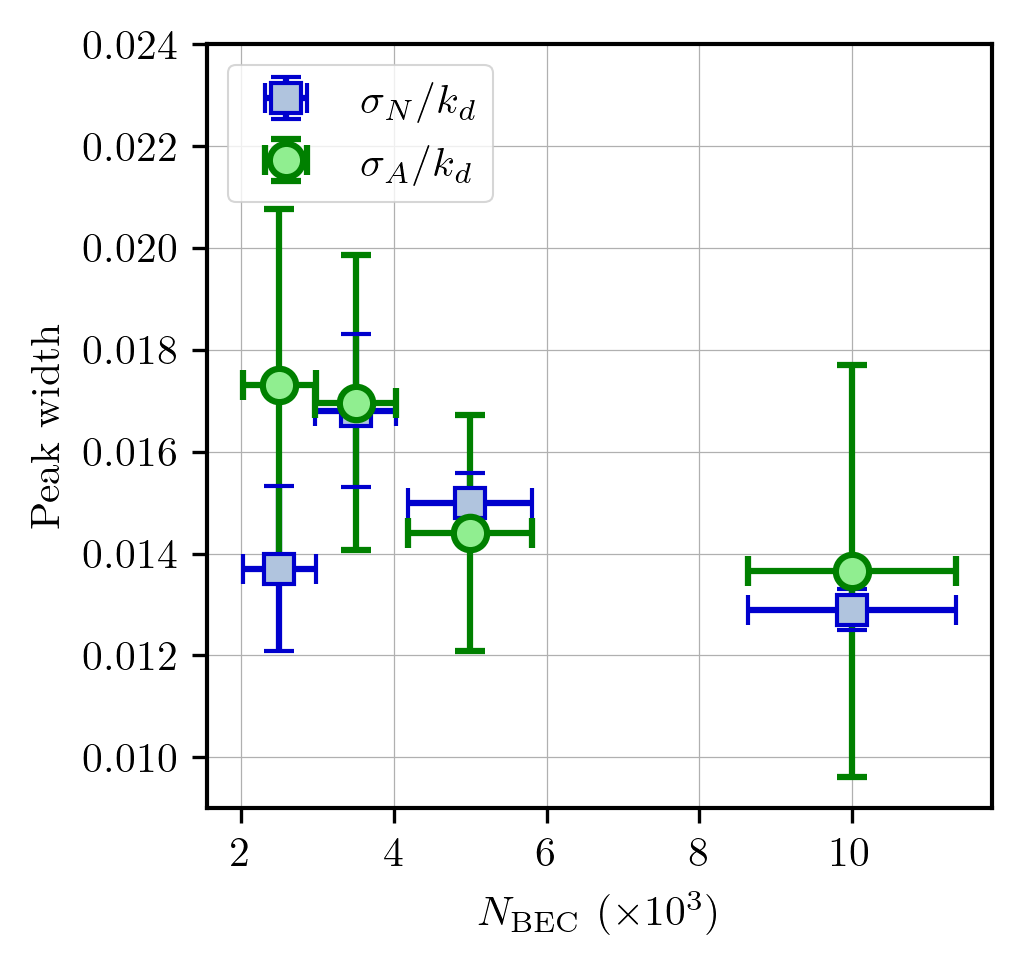
\includegraphics{Fig/Chapter4/widths_corrected.png}
    \caption[Corrected RMS widths of the anomalous and normal correlation peaks]{RMS widths of the anomalous (green) and normal (blue) correlation peaks corrected of the center-of-mass fluctuations. The widths $\sigma_A$ and $\sigma_N$ are no longer distinguishable within error bars, indicating that the temperature is too low to observe a clear separation of the anomalous and normal widths.}
    \label{fig:my_label}
\end{figure}


\section{Study of the amplitude of the correlation peaks}

We now move on to the study of the amplitude of the correlation peaks. Our objective will be to test how the predictions of Bogoliubov theory for the homogeneous case detailled in Chapter \ref{sec:chapter_1} hold for our experimental system with an optical lattice, as well as to provide further evidence of the quantum nature of the anomalous correlation signal.


% This method is illustrated on Fig-\ref{fig:integration_kk} for the bosonic bunching measurement for two temperatures as discussed in the previous section, as well as on Fig-\ref{fig:eta_vs_int_kmk} for different anomalous correlation signals.


\subsection{Normal correlations}

The prediction of the amplitude of the normal correlation peak is straightforward: as the statistics of the system are chaotic, we should observe a perfect bunching $\gtwo_N (\bm{0})=2$.
Coming back to the normal correlations plot of Fig-\ref{fig:kmk_temperature}, we observe that the amplitude is around 1.8, \ie slightly lower than 2. This is because of the transverse integration effects described in \ref{sec:transverse_integration}. We fit the dependency of the observed amplitude with transverse integration to extract the corrected amplitude value as explained in \ref{sec:transverse_integration} and illustrated in Fig.\ref{fig:integration_kk}. We obtain $g^{(2)}_N(\bm{0})=2.05(6)$ and $g^{(2)}_N(\bm{0})=2.09(5)$ for the high and low condensed fraction data sets respectively, consistently with Bogoliubov theory showing that the statistics of the system are chaotic. Note that our team conducted a thorough study of \kk correlations in the depletion of a lattice gas in \cite{cayla2020}, notably showing that we observe perfect bunching independently of the value of temperature as illustrated on Fig.-\ref{fig:bunching_vs_T}. 

\begin{figure}
    \centering
    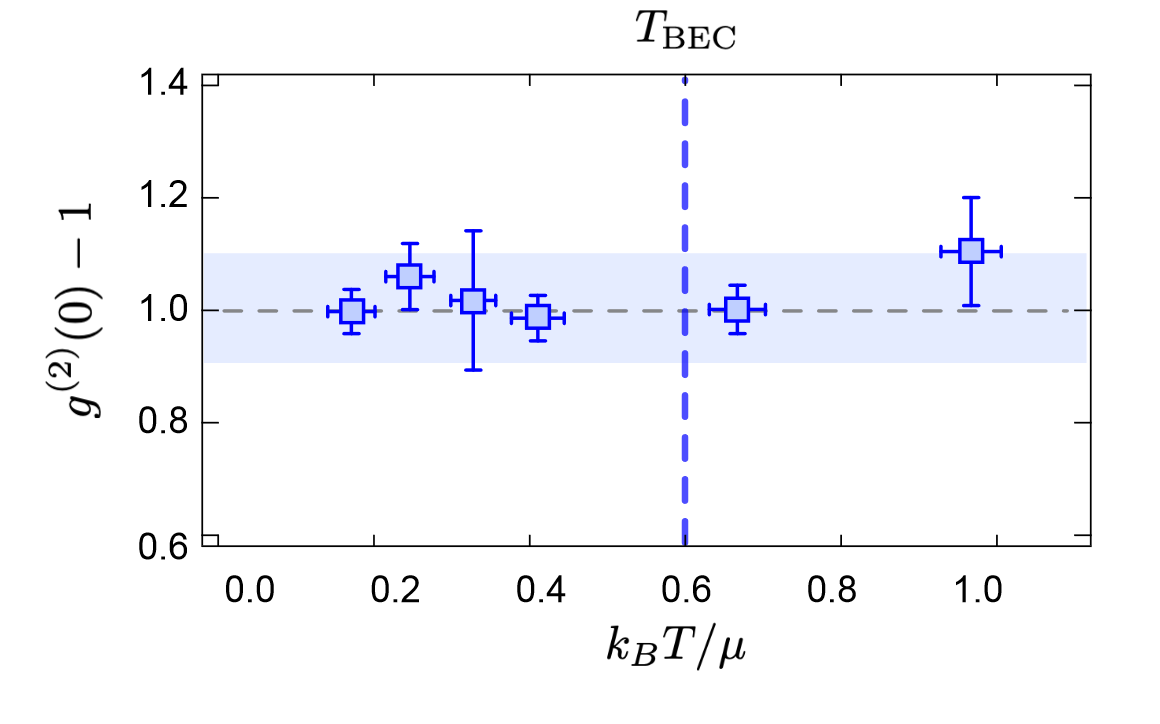
\includegraphics[width=0.7\textwidth]{Fig/Chapter4/bunching_vs_T.png}
    \caption[Bunching amplitude $g^{(2)}(0)-1$ as a function of the reduced temperature $\kB T/\mu$]{Bunching amplitude $g^{(2)}(0)-1$ as a function of the reduced temperature $\kB T/\mu$. The measurements are consistent with $g^{(2)}(0)=2$ at any temperature. The blue dashed line signals the temperature of the BEC $T_{\rm{BEC}}$.}
    \label{fig:bunching_vs_T}
\end{figure}



\subsection{Anomalous correlations}

\label{sec:amp_anomalous}

We now turn to analyzing the amplitude of the anomalous correlation peaks. As we have seen with the calculations developed in section \ref{sec:amp_parametric}, we can draw an analogy between the Bogoliubov weakly-interacting Bose gas and the non-degenerate parametric amplifier in Quantum Optics. While this analogy is direct if we were to work at zero temperature and have a fully quantum depletion where all atoms are correlated, we expect in our case that the amplitude of the anomalous correlation peak is reduced because of the presence of uncorrelated thermally depleted atoms. 

We showed in \ref{sec:amp_parametric} that the amplitude of the anomalous correlation peak of the non-degenerate parametric amplifier is expected to scale linearly with the inverse of what is called the average mode occupancy, {\it i.e.} the average number of photons per mode. In atomic physics, the analog to the average mode occupancy is the momentum density, {\it i.e.} the average number of atoms in a certain mode $\bm{k}$ that we can control by changing the total number of atoms $\NBEC$. As changing $\NBEC$ should not affect the balance between the quantum and thermal depletion, we should be able to observe that the amplitude of the anomalous correlation peak scales linearly with the inverse momentum density, despite not being at $T=0$.

Acutally, as explained in \ref{sec:accessing_depletion}, we measure correlation functions averaged over many modes in the momentum volume $\Omega_k$. The parameter setting the amplitude we observe is then the average momentum density $\bar{\rho}_{\Omega_k}$ defined as:

\begin{equation}
    \bar{\rho}_{\Omega_k}=\int_{\Omega_{k}} \rho({\bm k}) {\rm d}{\bm k}
\end{equation}

We have several possibilities to change the value of $\bar{\rho}_{\Omega_k}$:

\begin{itemize}
    \item Change the experimental parameters to load a different target total atom number $\NBEC$ in the optical lattice.
    \item Change the total atom number $\NBEC$ in the post-selection (see \ref{sec:post_selec}).
    \item Change the bounds of the integration volume $\Omega_k$.
\end{itemize}

We prepare 4 data sets using a combination of these 3 possibilities. We perform the experiment with a target loaded atom number $\NBEC=[2.5,5,10] \times 10^3$, and extract an additional set with $\NBEC=3.5 \times 10^3$ from the data intended for $\NBEC = 5 \times 10^3$ by changing the post-selection criterion. We also reduce $\Omega_k$ to momenta between $k_{\rm{min}} = 0.3 \ k_d$ and $k_{\rm{max}} = 0.7 \ k_d$, {\it i.e.} to a region where the depletion is lower. We thus reduce $\bar{\rho}_{\Omega_k}$ to observe higher amplitude values in hope of observing a clear violation of the Cauchy-Schwarz inequality (see \ref{sec:cs_inequality}).

The results are plotted on Fig.-\ref{fig:amplitude_vs_rhob} alongside the normal correlations amplitude for comparison. The horizontal error bars are the same as for Fig.-\ref{fig:width} while the vertical error bars are obtained from the fit error. We observe a linear scaling of the anomalous amplitude with the inverse average momentum density. On the other side, changing $1/\rhob$ does not change the chaotic nature of the system statistics, we thus observe $\gtwo_N (\bm{0})=2$ independently of the value of $\rhob$. Once again, the amplitudes were corrected of transverse integration effects as shown on Fig.-\ref{fig:eta_vs_int_kmk}. Note that the normal correlations amplitude is not shown for the point at the lowest average density as the amplitude does not increase at lower densities, resulting in a decrease of the signal-to-noise ratio.

\begin{figure}
    \centering
    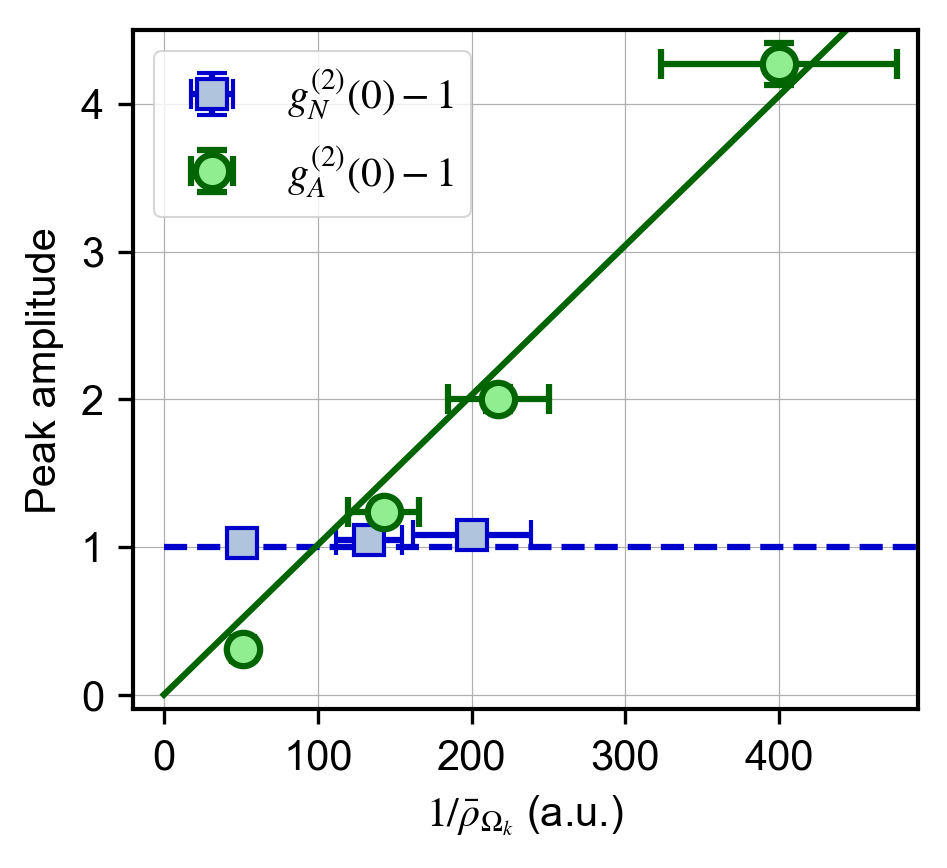
\includegraphics[width=0.65\textwidth]{Fig/Chapter4/amplitude_kmk.png}
    \caption[Amplitude of the correlation peaks versus the inverse average density $\rhob$]{Amplitude of the correlation peaks versus the inverse average density $\rhob$. We observe a linear scaling for anomalous correlations, while normal correlations stay constant and compatible with $\gtwo_N (\bm{0})=2$.}
    \label{fig:amplitude_vs_rhob}
\end{figure}

If we were at $T=0$, we remind from \ref{sec:amp_parametric} that the absolute value of the amplitude of the anomalous correlation peak should be $\gtwo_A (\bm{0}) = 2 + 1/\rhob$. Because of the temperature, we rather expect that the limit of $\gtwo_A (\bm{0})$ when $\rhob$ goes to infinity is a number between 1 and 2 whose value is determined by the balance between the quantum and thermal depletion. In the experiment, we found that a linear fit of $\gtwo_A (\bm{0})-1$ versus $1/\rhob$ with a zero intercept well matches the data, suggesting that the fraction of quantum depletion is actually very small. In fact, this quantity can be determined more precisely as we will now see.


\subsubsection{Discussion on the detected number of atom pairs}

The absolute value of the amplitude can be used to extract the number of detected \kmk pairs, following the procedure previously described in \ref{sec:benchmark_algo}. For the data set $\NBEC=5 \times 10^3$, $f_c=84 \%$, we find that we detect on average $0.5$ pairs per shot, for roughly $N_{\Omega_k}=100$ atoms detected in $\Omega_k$. This number can be used to calculate the fraction of quantum depleted atoms in the overall depletion condensate that we will write $\alpha_Q$. We first assume that all atoms in the quantum depletion form a \kmk pair and that atoms forming a \kmk pair necessarily belong to the quantum depletion. We then have:

\begin{equation}
    2N_{\rm{pairs}}= N_{\Omega_k} \alpha_{\rm{MCP}} \alpha_Q
    \label{eq:Npairs}
\end{equation}

\noindent This equation can be understood as follows. We initially have a given number of depleted atoms in $\Omega_k$ that we detect only a fraction of because of the MCP detection efficiency. This number is $N_{\Omega_k}$ which already includes the detection efficiency per atom $\alpha_{\rm{MCP}}$. In all these atoms, only the fraction of quantum depleted ones $\alpha_Q$ will be \kmk paired. In addition, we miss some pairs when detecting only one atom of the pair because of the detection efficiency, hence the addition of $\alpha_{\rm{MCP}}$ in the formula.

We use equation \ref{eq:Npairs} to evaluate $\alpha_Q$ and find $\alpha_Q \simeq 1.6 \%$. Using a $T=0$ Gutzwiller approach (see \ref{sec:gutzwiller}), we estimate the quantum depletion to be $5\%$ and infer that the thermal depletion must then be $\simeq 10\%$ as the overall condensed fraction is $f_c=84 \%$. This would mean that we should rather have $\alpha_Q \simeq 33 \%$, so more than an order of magnitude larger than our experimental measurement. We perform the same measurements for data sets with different total atom numbers with the results shown in Table-\ref{tab:nb_pairs}, and observe that the value of $\alpha_Q$ does not significantly change. While this is consistent with the fact that we are able to observe a linear scaling of $\gtwo_A (\bm{0})$ with $1/\rhob$ and that $\gtwo_A (\bm{0})-1$ tends to almost zero when $1/\rhob$ goes to infinity, there is significant discrepancy with the estimation of the Gutzwiller approach. Finding a clear explanation for this discrepancy remains an open question and would require an extensive theoretical work far beyond the scope of this thesis. We can however suggests a few possible explanations:

\begin{itemize}
    \item While we estimate the total quantum depletion, we cannot count all the pairs as some of them are located in the region of the BEC removed from the analysis. At the moment, we do not have the theoretical tools necessary to determine how many pairs are removed that way.
    \item Some of the pairs that we detect are located close to the edge of the first Brillouin where the relation dispersion becomes flat. It is then not so clear whether Bogoliubov's theory predictions for an homogeneous gas should quantitatively hold, as the Bogoliubov dispersion relation is an increasing function of the momentum.
    % \item The balance between thermal and quantum depletion depends from the momentum $k$. It is then not so clear of what this number should be averaged over $\Omega_k$. In addition, a significant amount of \kmk pairs can be located in the low $k$ region that we remove from the analysis, thus reducing the number of detected pairs.
    % \item Dispersion relation of the lattice \NOTE{COMPLETER}
    % \item Is is also not so clear how the pairs are projected into the different Brillouin zones when performing the time-of-flight measurement. This could also makes us miss some pairs (\NOTE{BOF}).
\end{itemize}

\begin{table}[]
    \centering
    {\rowcolors{2}{white}{MainColor!12}
    \begin{tabular}{ c|c|c }
        {\color{MainColor} $\bm{\NBEC}$} & {\color{MainColor} $\bm{N_{\rm{pairs}}/N_{\rm{runs}}}$} & {\color{MainColor} $\bm{\alpha_Q$}}  \\
        $2.5 \times 10^3$ & $0.15$ & $1.5 \%$ \\ 
        $5 \times 10^3$ & $0.5$ & $1.6 \%$ \\ 
        $10 \times 10^3$ & $0.9$ & $1.2 \%$ \\ 
    \end{tabular}}
    \caption{Average number of detected \kmk pairs per experimental run and fraction of quantum depleted atoms in the depletion for different total atom numbers.}
    \label{tab:nb_pairs}
\end{table}



In conclusion, the observed linear scaling is consistent with what is predicted by Bogoliubov theory and gives us another argument showing that the observed anomalous correlation signal is linked to the quantum depletion. The absolute value of the amplitude cannot however be understood in the framework of the Bogoliubov theory \cite{butera2020} that does not account for all the specificities of our experiment, such as the presence of the lattice. In fact, evaluating this number is currently beyond what is possible to calculate, making our experiment an example of quantum simulation.


\section{Towards measuring entanglement}

As we underlined in the first chapter of this thesis, it would be of great interest to characterize how entanglement emerges in at-equilibrium many-body systems such as the one we are working with here. Although we do not have all the experimental tools to claim that we are indeed seeing entanglement in our experiment yet, we nevertheless observe clear signatures of quantum phenomena that hints towards it as we will discuss now.



\subsection{Relative number squeezing}

If we were in the perfect situation $T=0$ were the depletion is fully quantum, the populations in modes $\bm{k}$ and $-\bm{k}$ would be totally correlated so that the quantity $N(\bm{k})-N(-\bm{k})$ is non-fluctuating and always equal to 0. This is obviously not the case in our finite temperature experiment where a significant fraction of the depletion is thermal and thus uncorrelated. However, we expect the \kmk correlations to reduce the fluctuations of $N(\bm{k})-N(-\bm{k})$. This is what we call \textbf{relative number squeezing}, similar to --but not to be confused with-- regular squeezing \cite{walls1983squeezed} that denotes the reduction of the fluctuations of an operator ({\it e.g} momentum) under the Heisenberg limit at the expense of increased fluctuations for the conjugate operator ({\it e.g} position).

% A slightly higher level proof of quantum behavior than the violation of the Cauchy-Schwarz inequality is observing \textbf{squeezing}. Before going into our experimental details and observations, let us briefly remind what is squeezing is.

% In quantum mechanics, the maximum precision with which one can hope to measure two conjugate quantities such as position and momentum is bound by the very famous Heisenberg inequality:

% \begin{equation}
%     \Delta x \Delta p \geq \frac{\hbar}{2}
% \end{equation}

% In most cases, notably the quantum harmonic oscillator ground state $\ket{0}$ and coherent states $\ket{\alpha}$, the minimum uncertainties values saturating the Hesienberg inequality are the same for the two conjugate quantities $\Delta x_{g} = \Delta p_g$. The specificity of squeezed states is that the uncertainty one of the quantities has been reduced below the lower limit of the ground state, at the detriment of the uncertainty of the conjugate quantity. If we were to represent the uncertainty in quadrature space, we would get a perfect circle for a coherent state and a "squeezed" circle, {\it i.e.} an ellipse, for a squeezed state, hence the name. \NOTE{BIBLIO/EXEMPLES}, \NOTE{VOIR AVEC CHAPITRE 1 OU METTRE CA}

% A well-known example of how to obtain squeezing is the non degenerate parametric amplifier in non linear quantum optics. \NOTE{A faire quand le chapitre 1 est fait}

 The idea is then to measure the statistics of the difference of atom numbers in modes $\bm{k}$ and $-\bm{k}$ that we will refer to as $N(\bm{k})$ and $N(-\bm{k})$. For one of the modes, the fluctuations of the number of atoms are set by the \textbf{shot noise} and follow a Poisson law. The particularity of the Poisson law for a random variable is that the variance of the variable is equal to its mean, giving for instance for mode $\bm{k}$:

\begin{equation}
    \sigma_{N(\bm{k})}^2 =\mean{N(\bm{k})^2}-\mean{N(\bm{k})}^2 = \mean{N(\bm{k})}
\end{equation}

What can we tell of the statistics of the number difference in two modes $\bm{k}$ and $\bm{k}'$, $N(\bm{k}) - N(\bm{k}')$? If the populations in the two modes are totally uncorrelated, the difference of two independent Poissonian random variables is Poissonian as well and we then get:

\begin{equation}
    \sigma_{N(\bm{k})-N(\bm{k}')}^2 = \mean{N(\bm{k})-N(\bm{k}')}
\end{equation}

If we now chose $\bm{k}'=-\bm{k}$, we expect the \kmk correlations present in the depletion to reduce the fluctuations of the number difference, yielding what is called a \textbf{sub-Poissonian} law. Just like the \kmk correlation signal is lost with temperature, we expect that the reduction of the number difference fluctuations becomes smaller and smaller as temperature increases, increasing the fraction of thermally, uncorrelated, depleted atoms. 

Our goal is then to measure $\sigma_{N(\bm{k})-N(-\bm{k})}$ and see whether it is smaller than the expected value for a Poisson law. To this end, we define a convenient quantity that we call the squeezing parameter $\xi$: 

\begin{equation}
    \xi_{\bm{k},\bm{k'}}^2=\frac{\langle (N_{\bm{k}} - N_{\bm{k'}})^2 \rangle - \langle N_{\bm{k}} - N_{\bm{k'}} \rangle^2}{\langle N_{\bm{k}} \rangle + \langle N_{\bm{k'}} \rangle}
\end{equation}

This squeezing parameter to the square is simply the standard deviation of the number difference normalized by the expected standard deviation for uncorrelated variables. Therefore, we expect $\xi^2_{\bm{k},\bm{k}'}=1$ if there are no correlations between modes $\bm{k}$ and $\bm{k'}$, and $\xi^2_{\bm{k},\bm{k}'} < 1$ if the modes populations are correlated.

To evaluate $\xi^2$, we record for each experimental shots the number of detected atoms in cubic boxes paving the entire integration volume $\Omega_k$. Intuitively, we could set the size of the boxes to match that of a mode. If we define the volume of a mode as the volume of a sphere whose radius is the two-particle correlation length $l_c$ obtained from the normal correlation function width with $l_c = \sqrt{2} \sigma_N$ \cite{carcy2019momentum}, we obtain that there are $N_{\rm{mode}} = 1.5 \times 10^4$ modes in $\Omega_k$, \ie on average $\sim 0.01 \ \text{atoms/mode/run}$ (for $\NBEC=5 \times 10^3$) which is way to small to have proper statistics to evaluate $\xi^2$. We then chose a size of $(0.3 \ k_d)^3$. The average numbers of detected atoms per shot are $\sim 100$, $\sim 240$ and $\sim 360$ for the data sets with $f_c=84\%$, $f_c=55\%$ and $f_c=29\%$ respectively, meaning that the average number of atom per box are $0.8$, $1.92$ and $2.88$ respectively. Having access to the atom number for each of the $\sim 2000$ runs at various values of $\bm{k}$, we compute the squeezing parameter between different pairs of boxes as illustrated on Fig.-\ref{fig:squeezing}, either correlated or uncorrelated for reference. The measured values of $\xi^2$ are averaged over all possible pairs of boxes for a given configuration. The uncertainty on $\xi^2$ is evaluated statistically on all the $\xi^2$ values obtained on the 62 different pairs of boxes and defined as the standard error.

\begin{figure}
    \centering
    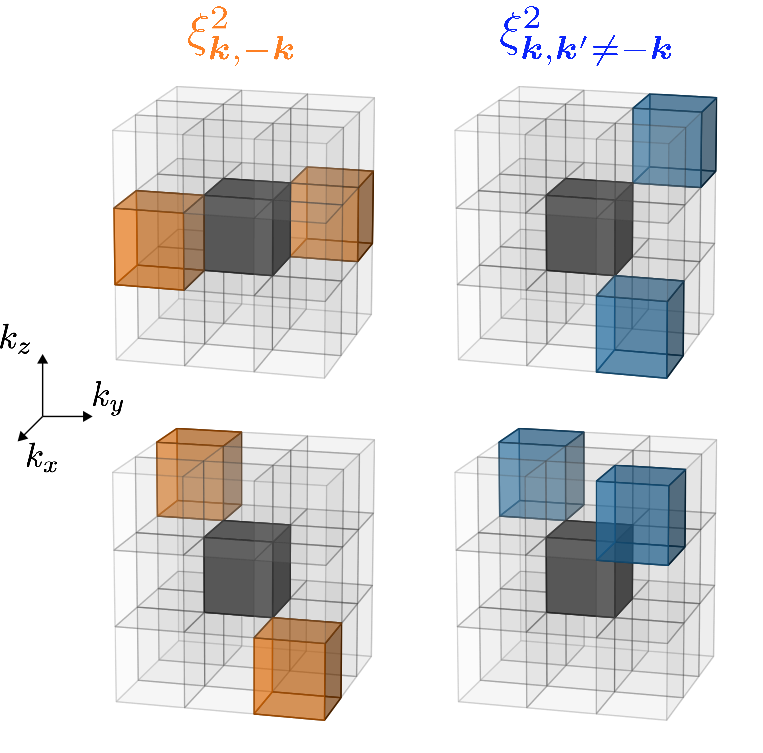
\includegraphics[width=0.7\textwidth]{Fig/Chapter4/squeezing.png}
    \caption[Relative number squeezing measurement]{Relative number squeezing measurement. The number of detected atoms in cubic boxes are recorded for each experimental run. We compute the squeezing parameter $\xi$ between correlated (orange) boxes as illustrated on the right, or uncorrelated (blue) boxes on the left. The central black box corresponds to the BEC, removed from the analysis.}
    \label{fig:squeezing}
\end{figure}

The results are summarized in Table \ref{tab:squeezing} and Fig.-\ref{fig:squeezing_graph}. For the low-temperature, high condensed fraction data, we are indeed able to observe a small relative number squeezing within the errorbars. Note that this number squeezing is small compared to that found in discrete (spin) variables experiments \cite{bucker2011,esteve2008squeezing, pezze2018} as it is inherently limited by the uncorrelated thermally depleted atoms and the detection efficiency. For uncorrelated modes, the squeezing parameter is very slightly above 1, highlighting that the correlations indeed reduce the fluctuations of the number difference. For higher temperatures (lower condensed fraction), no relative number squeezing is observed as the correlations are drowned out. In addition, we see that the squeezing parameter increases as we increase the temperature. This is due to global atom number fluctuations of the order of $15\%$ in our experiment. At low temperature, there are few detected atoms per box and the shot noise is thus large and dominating the total atom number fluctuations. On the opposite, at higher temperatures, the number of depleted atoms increases, reducing the shot noise. The contribution of total atom number fluctuations is then not negligible anymore and increase the fluctuations of the number difference, higher than what is expected for a Poisson law, explaining why we observe $\xi^2 > 1$.

\begin{table}[ht!]
    \centering
    {\rowcolors{2}{white}{MainColor!12}
    \begin{tabular}{ c|c|c }
        {\color{MainColor} $f_c$} & {\color{MainColor}$\xi^2_{\bm{k},-\bm{k}}$ } & {\color{MainColor}$\xi^2_{\bm{k},\bm{k}'}$} \\
        0.84 & 0.992(3) & 1.004(3) \\
        0.55 & 1.017(4) & 1.017(3) \\
        0.29 & 1.040(5) & 1.045(5) \\

    \end{tabular}}
    \caption{Experimental values of the squeezing parameter for correlated and uncorrelated modes and different condensed fractions.}
    \label{tab:squeezing}
\end{table}

\begin{figure}
    \centering
    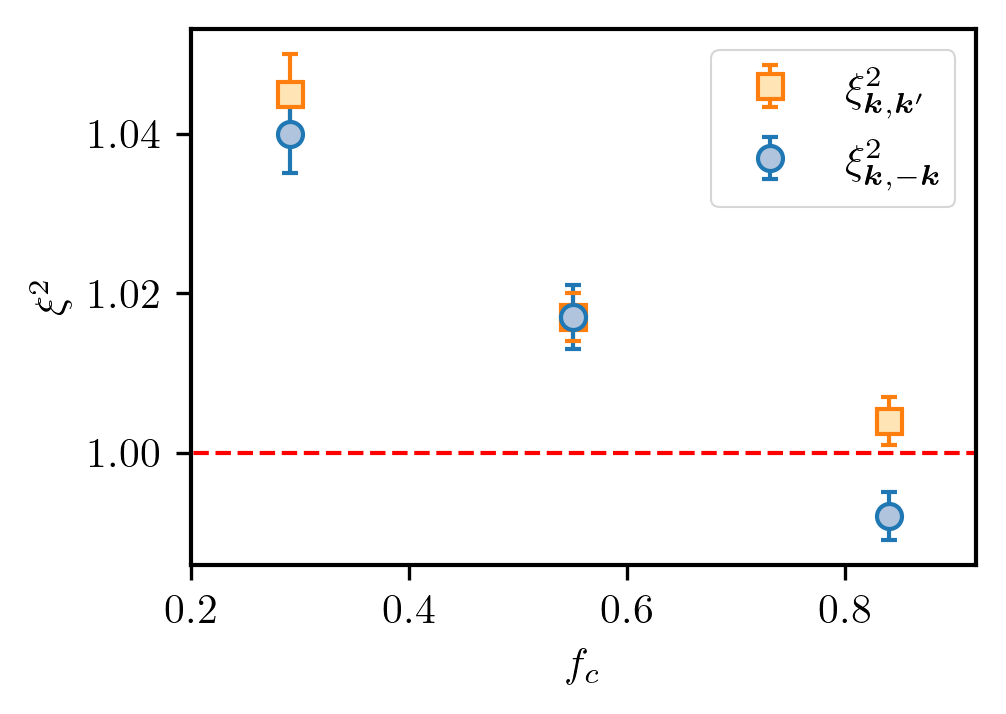
\includegraphics[width=0.7\textwidth]{Fig/Chapter4/squeezing_graph.png}
    \caption[Squeezing parameter $\xi^2$ as a function of the condensed fraction $f_c$ for correlated and uncorrelated modes]{Squeezing parameter $\xi^2$ as a function of the condensed fraction $f_c$ for correlated and uncorrelated modes. The red line indicates the expected value $\xi^2=1$ for Poissonian number difference fluctuations. At $f_c=0.84$, a clear difference is observed between $\xi^2_{\bm{k},-\bm{k}}$ and $\xi^2_{\bm{k},\bm{k}^{\prime}}$ and relative number squeezing is observed as $\xi^2_{\bm{k},-\bm{k}} < 1$. The difference between $\xi^2_{\bm{k},-\bm{k}}$ and $\xi^2_{\bm{k},\bm{k}^{\prime}}$ disappears as $f_c$ decreases as the effect of \kmk correlations gets drowned out. The global increase in the value of $\xi^2$ when $f_c$ decreases is caused by total atom number fluctuations (see main text).}
    \label{fig:squeezing_graph}
\end{figure}


% \begin{table}[]
%     \arrayrulecolor{black}
%     \centering
%     \begin{tabular}{|c|c|c|}
%         \hline
%         $f_c$ & $\xi^2_{\bm{k},-\bm{k}}$ & $\xi^2_{\bm{k},\bm{k}}$ \\
%         \hline
%         0.84 & 0.992(3) & 1.004(3) \\
%         \hline
%         0.55 & 1.017(4) & 1.017(3) \\
%         \hline
%         0.29 & 1.040(5) & 1.045(5) \\
%         \hline
%     \end{tabular}
%     \caption{Experimental values of the squeezing parameter for correlated and uncorrelated modes and different condensed fractions.}
%     \label{tab:squeezing}
% \end{table}

\subsection{Experimental violation of the Cauchy-Schwarz inequality}

We have previously shown in \ref{sec:cs_inequality} how the Cauchy-Schwarz inequality writes with creation and annihilation operators and translated it in terms of correlation functions. Translated to anomalous and normal correlations function discussed in this chapter, the Cauchy-Schwarz inequality writes:

\begin{equation}
    \gtwo_A (\bm{k},-\bm{k}) \leq \gtwo_N (\bm{k},\bm{k})
\end{equation}

We thus have a clear violation of the Cauchy-Schwarz inequality with our experimental data on 3 different data points, with a maximum violation of $5.27(8) > 2.09(5)$ (Fig.-\ref{fig:amplitude_vs_rhob}). This adds up to the list of quantum signatures in the anomalous correlation signal.

As discussed in \ref{sec:cs_inequality}, violating the Cauchy-Schwarz inequality equals fulfilling the Busch-Parentani criterion to prove entanglement, provided that certain conditions are fulfilled. The first one is that the statistics of the system must be thermal chaotic. This is something that we have experimentally verified by measuring $\gtwo_N (\bm{0}) = 2$. The second condition is to have $\langle a^{\dagger}_{\bm k} a_{-\bm k} \rangle=0$. While this is true in Bogoliubov theory and would be reasonable to assume in our experiment, this is not something that we have experimentally measured and that therefore forbids us to claim that we observe entanglement in momentum-space. This correlator could be measured using an atomic inteferometer setup \cite{dussarrat2017two,kasevich1991atomic,lopes2015atomic} using Bragg diffraction \cite{martin1988bragg} to produce atom mirrors and beam splitter. This would however require that we upgrade our experimental apparatus to have the required lattice beam to implement the proper Bragg diffraction scheme. Nevertheless, proving the presence of entanglement in momentum-space in many-body equilibrium systems would be a significant result that motivates such experimental work in the near future. 


% The very famous Cauchy-Schwarz inequality has seen countless applications in mathematics and physics. What will most interest us here is its formulation in the framework in probability theory. In classical physics, with two fluctuating quantities $I_1$ and $I_2$, the Cauchy-Schwarz inequality writes:

% \begin{equation}
%     \mean{I_1 I_2} \leq \sqrt{\mean{I_1^2} \mean{I_2^2}}
% \end{equation}

% This inequality can be rewritten with creation/annihilation operators to work with two-body correlation functions. For simplicity sake, let's consider only two modes 1 and 2. We introduce the notation $G^{(2)}_{i,j} = \mean{\hat{a}(i)^{\dagger} \hat{a}(j)^{\dagger} \hat{a}(i) \hat{a}(j)}$. The Cauchy-Schwarz inequality becomes \cite{kheruntsyan2012violation,walls2008}:

% \begin{equation}
%     G^{(2)}_{1,2} \leq \sqrt{G^{(2)}_{1,1} G^{(2)}_{2,2} }
% \end{equation}

% If we now chose mode $1 \rightarrow \bm{k}$, mode $2 \rightarrow -\bm{k}$ and consider a symmetrical case with $\mean{\hat{a}^{\dagger}(\bm{k}) \hat{a}(\bm{k})}=\mean{\hat{a}^{\dagger}(-\bm{k}) \hat{a}(-\bm{k})}$ (consistent at $T=0$ where the depletion is fully quantum and exclusively populated in pairs), we obtain $G^{(2)}_{\bm{k},\bm{k}}=G^{(2)}_{-\bm{k},-\bm{k}}$ and finally:

% \begin{equation}
%     \gtwo_A (\bm{k},\bm{-k}) \leq \gtwo_N (\bm{k},\bm{k})
% \end{equation}

% Therefore, the Cauchy-Schwarz inequality states that the cross-correlation amplitude between opposite momenta cannot exceed the amplitude of the auto-correlation with a classical model. As shown on Fig-.\ref{fig:amplitude_vs_rhob}, the experimental amplitude of the anomalous correlations goes significantly higher than for normal correlations, thus clearly violating the Cauchy-Schwarz inequality for classical quantities: we are thus observing quantum correlations. As developed in \cite{kheruntsyan2012violation}, violating the Cauchy-Schwarz inequality is one of the easiest way to prove the presence of non-classical correlations and represents a first, necessary step towards obtaining more significant results such as proving the presence of entanglement.

\section{Preliminary study: dependency of the correlation signals with k}

As we have seen throughout this chapter, the balance between the quantum and thermal depletion and thus the temperature plays an important role in both the amplitude of the anomalous correlation function (see \ref{sec:kmk_temperature}) as well as the width of the normal correlation function (see \ref{sec:width_correlation_theo}). Interestingly, the ratio of the quantum and thermal depletion changes with the momentum value $k$ as they have different momentum scales set by the strength of the interactions and the temperature respectively. Whereas we have until now kept the integration volume $\Omega_k$ as large as possible, it would be then be interesting to reduce it and move it around momentum-space to see whether we can observe variations of the characteristics of the correlation signals depending on the momentum value around which $\Omega_k$ is centered. Note that the study presented in this section is preliminary and still an on-going work.

\subsection{Evolution of the amplitude of the anomalous correlations with k}

As far as the amplitudes of the correlation signals are concerned, there is not much too learn studying the dependency of the amplitude of the normal correlation signal with $k$ as it only reveals the chaotic statistics of the system that are unaffected by temperature and are thus independent of $k$. We will then focus solely on the amplitude of the anomalous correlation function. 

We repeat the analysis procedure described before for various integration volumes $\Omega_k$ that we set by changing its boundaries $k_{\rm{min}}$ and $k_{\rm{max}}$ (see \ref{sec:accessing_depletion}). In practice, we chose the couples $[k_{\rm{min}},k_{\rm{max}}]=[0.15,0.3],[0.2,0.35],...,[0.35,0.5] \ k_d$, scanning the first Brillouin zone. As $\Omega_k$ is smaller than for previous analysis showed in this chapter, the signal to noise ratio is not sufficient to extract a value of the amplitude for a large panel of transverse integration values to extract the amplitude corrected from transverse integration as described in \ref{sec:transverse_integration}. We will then rather plot the raw amplitude $\eta_A$ for a fixed transverse integration $\Delta k_{\perp}=3 \times 10^{-2} \ k_d$. In addition, when changing $\Omega_k$, we also change the value of $\rhob$ that affects the amplitude of the anomalous correlation peak. We therefore ``normalize'' this effect by plotting the quantity $\eta_A \times \rhob$ that should only reveal the effect of the variations of the balance between the quantum and the thermal depletion.

We plot on Fig.-\ref{fig:eta_A_vs_k} $\eta_A \times \rhob$ as a function of $k_{\rm{center}}=(k_{\rm{min}}+k_{\rm{max}})/2$ for the data sets with $\NBEC= 5 \times 10^3$ and holding times $5 \ \rm{ms}$ and $200 \ \rm{ms}$. We observe that for the coldest data set, $\eta_A \times \rhob$ increases with $k$, indicating that the ratio of the quantum depletion to the thermal depletion increases with $k$ in the momentum range that we probe. When the temperature increases (orange points of Fig.-\ref{fig:eta_A_vs_k}), the thermal depletion increases and populates higher momentum modes, meaning that the ratio of the quantum depletion to thermal depletion should not increase as fast or even possibly decrease with $k$ if the temperature is high enough. This is what we observe on the experimental data for which $\eta_A \times \rhob$ increases much slower for the heated data. We note that as the overall density of the depletion is higher at low $k$ reducing the amplitude of the anomalous correlation function, we were not able to observe the correlation signal for $[k_{\rm{min}},k_{\rm{max}}]=[0.15,0.3],[0.2,0.35]$ with the $200 \ \rm{ms}$ holding data.

\begin{figure}
    \centering
    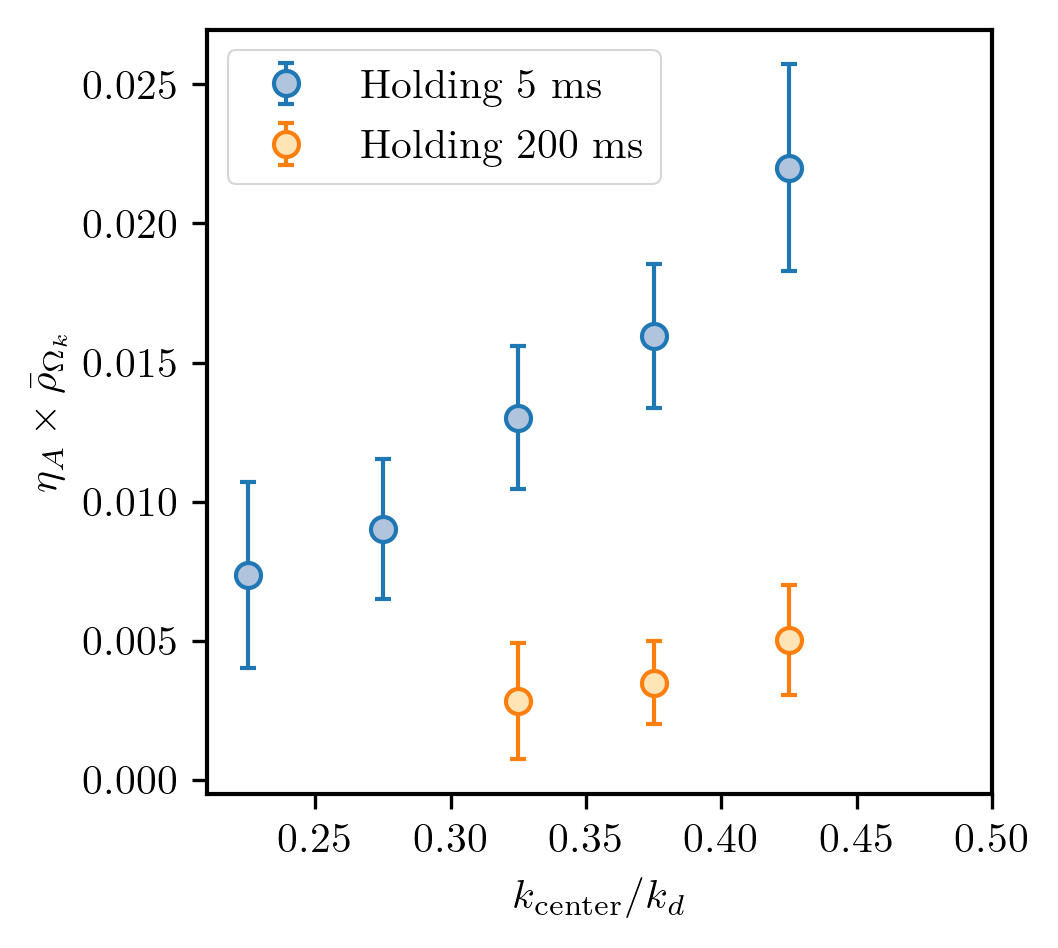
\includegraphics[width=0.7\textwidth]{Fig/Chapter4/eta_A_vs_k.png}
    \caption[Evolution of the anomalous correlations amplitudes with $k$]{Raw amplitude $\eta_A$ mutiplied by the average density $\rhob$ as a function of $k_{\rm{center}}$ for two data sets as different temperatures.}
    \label{fig:eta_A_vs_k}
\end{figure}

While this kind of data could in principle be used to find the temperature of the experiment, we must for the moment only restrict ourselves to the qualitative description we have just given for lack of a precise theory of the correlations in an optical lattice.

\subsection{Evolution of the width of the normal correlations with k}

As seen in \ref{sec:width_anomalous_theo}, the width anomalous correlation peak is essentially constant with $k$ and therefore does not bring much additional information. On the contrary, in analogy with the amplitude of the anomalous correlation peak, the width of the \textbf{normal} correlation peak $\sigma_N$ is strongly dependent from the balance between the quantum and thermal depletion (see \ref{sec:width_normal_theo}). As described in the previous paragraph, we measure $\sigma_N$ for different integration volumes $\Omega_k$. This time, we choose $[k_{\rm{min}},k_{\rm{max}}]=[0.15,0.25],[0.2,0.3],...,[0.4,0.5] \ k_d$.

We plot on Fig.-\ref{fig:sigma_N_vs_k} $\sigma_N$ as a function of $k_{\rm{center}}$ for 3 data sets: the first one with $\NBEC=10 \times 10^3$ and a holding time of $5 \ \rm{ms}$ and the other two with $\NBEC=5 \times 10^3$ and holding times $200 \ \rm{ms}$ and $500 \ \rm{ms}$ respectively to increase the temperature. We note that we deliberately chose a data set with a higher atom number for the lowest holding times to increase the number of depleted atoms and have a proper signal to noise ratio. Unfortunately, we observe that the error bars are too large to capture any possible variations of $\sigma_N$. It then seems after this preliminary that $\gtwo_A (\bm{0})$ is a better suited probe than $\sigma_N$ to understand the variations of the balance between the quantum and thermal depletion with $k$ in our experiment.

\begin{figure}
    \centering
    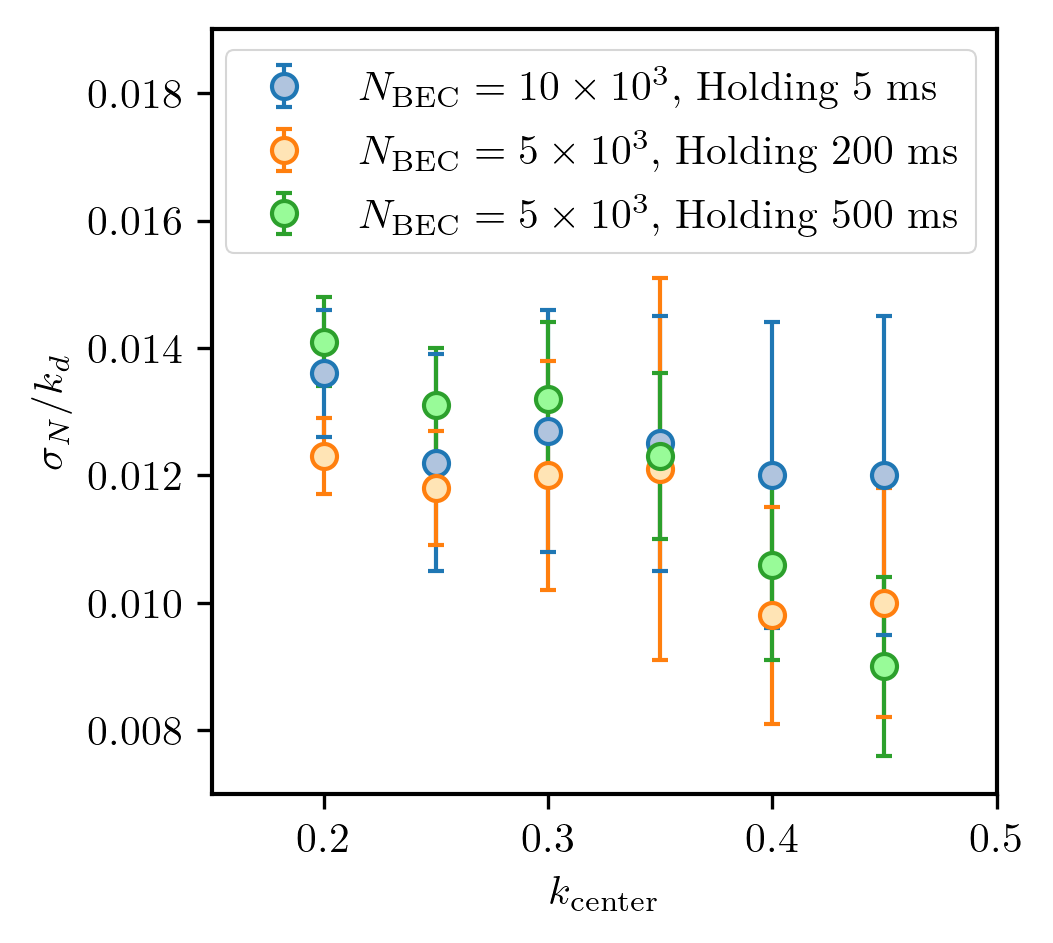
\includegraphics[width=0.7\textwidth]{Fig/Chapter4/sigma_N_vs_k.png}
    \caption[Evolution of the normal correlation peak width $\sigma_N$ with $k$]{Normal correlation peak width $\sigma_N$ as a function of $k_{\rm{center}}$ for various data sets at different temperatures.}
    \label{fig:sigma_N_vs_k}
\end{figure}

As mentioned in the introduction to this section, the results presented here are still quite preliminary and there are quite a few points that need further investigation, notably why the number of detected pair is lower than expected, constituting an interesting prospect for the near future.

\section{Conclusion}

We have reached the end of our investigation of two-body correlation in the depletion of weakly interacting Bose gases. To sum things up, let us remind the main steps of the work conducted during this thesis and its main results.

\begin{itemize}
    \item We decided to try to detect experimentally the \kmk pairs of the quantum depletion predicted by the Bogoliubov theory of the weakly-interacting Bose gas, as this phenomenon is one of the conceptually simplest non-trivial, many-body, quantum correlation effect. By conducting this study, we hope to better understand the physics of many-body equilibrium states and how correlations and entanglement emerge through the combined effects of interactions and quantum fluctuations.
    \item We based our experimental procedure on an experimental setup producing $\He$ BECs  implementing a 3D single-atom resolved electronic detection technique. We decided to use an optical lattice to enter the low-temperature regime dominated by interactions to ensure a sufficient level of quantum depletion so that the \kmk pairs can be properly detected.
    \item We completed previous benchmarking measurements \cite{cayla2018single} by measuring two-body time-of-flight collisions with large number of atoms in the lattice. From this, we were able to conclude that two-body collisions are negligible for the typical number of atoms used in our correlation measurement experiments. This validates the ballistic relation linking the momentum of the in-trap to their detected position after the TOF.
    \item We measured the temperature of the gas at different amplitudes of the lattice potential to certify the adiabatic preparation of the system.
    \item We implemented a two-photon Raman transfer scheme to replace the previous RF transfer, improving the detection efficiency by a factor 2.
    \item We adapted an existing algorithm to make it suited to extract the \kmk correlation signal from the experimental data and benchmarked it with collision spheres data.
    \item We were able to successfully observe anomalous and normal correlation signals in various data sets with different total atom numbers. We validated that the observed anomalous correlation signal is linked to the \kmk pairs of the quantum depletion with the following points:
    \begin{itemize}
        
        \item The signal is lost with temperature, contrary to the normal correlation signal that reveal the chaotic statistics of the system, unaffected by temperature.
        \item The width of the anomalous correlation peak matches the numerical calculations of \cite{butera2020} when accounting for center-of-mass fluctuations.
        \item $\gtwo_A(\bm{0})$ scales linearly with the inverse average momentum density $\bar{\rho}_{\Omega_k}$, while $\gtwo_N(\bm{0})$ remains constant.
        \item Relative number squeezing between correlated boxes at opposite momenta is observed.
        \item A violation of the Cauchy-Schwarz inequality $\gtwo_A(\bm{0}) \gg \gtwo_N(\bm{0})$ is reported.
        
    \end{itemize}
\end{itemize}

This experimental observations are an encouraging first step towards more ambitious correlation measurements. One of our short term objective is to study the Mott transition and look for complex correlation patterns involving several particles not predicted by simple theoretical treatment such as Bogoliubov theory. As there is currently no theory describing this kind of physics, this represents quite a fascinating prospect that would really put our experiment in the field of quantum simulation. In addition, a more long term prospect would be to improve our experimental setup to bring the fermionic isotope $^3 \mathrm{He}^*$ to quantum degeneracy to perform momentum correlations measurements with fermions and study BEC-BCS crossover physics. A notably important result would be to observe the \kmk pairing of a Cooper pair \cite{cooper1956bound}. Observing the \kmk pairing of the quantum depletion shows us that we are indeed capable of seeing \kmk pairing with our experiment and constitutes a small step towards this result.




\chapter{Towards measuring Tan's contact in 1D gases}

\section{Tan's contact for 1D gases}

To understand what Tan's contact is, we consider two atoms with contact interactions in 1D. 

\section{Theoretical study}

\subsection{Effect of temperature}

\subsection{Effect of the interaction parameter}

\section{Experimental realisation of 1D gases with the optical lattice}

The main idea to experimentally study 1D physics is to ``freeze'' the degrees of freedom of the atoms in two directions of space. To do so, the easiest solution is to use a harmonic trapping potential with trapping frequencies $\omega_{\perp}$ high enough so that the energy difference $\Delta E =\hbar \omega_{\perp}$ between the ground-state and the first excited state is much larger than the typical energy of the atoms $\Delta E \gg \kB T, \mu$. Such high trapping frequencies are accessible in our experiment thanks to the optical lattice. Instead of using the 3 pairs of countra-propagating beam as we did so far, we use only 2 to produce a 2D lattice. Interestingly, the total laser power is divided amongst 2 pair of beams instead of 3, meaning that we can reach much higher values of the lattice depth, typically up to $s=30$. In the direction where there is no lattice, the trapping potential results from the Gaussian shape of the beams and has a trapping frequency $\omega_{\rm{1D}} =2 \pi \times 140 \sqrt{s} = 2 \pi  \times 713 \ \rm{Hz}$ for $s=26$. In the other 2 directions, the trapping frequency is however very large as a result of the lattice interference pattern $\omega_{\perp} \simeq 200 \ \rm{kHz}$, which is much larger than the energy of the atoms $\kB T, \mu \simeq 25 \ \rm{kHz}$ with typical experimental parameters.

\begin{figure}
    \centering
    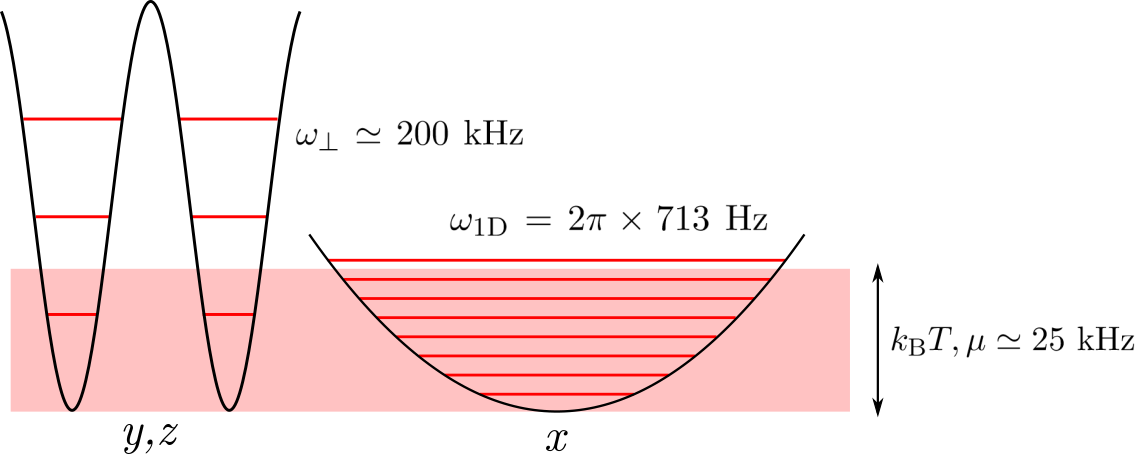
\includegraphics[width=0.9\textwidth]{Fig/Chapter5/1D_config.png}
    \caption{Configuration of the optical lattice to produce 1D tubes. In the transverse direction, the lattice interference pattern creates a confining potential that can be approximated to a harmonic potential near the center of the site. The trapping frequency is high enough so that the degree of freedom of the atoms in these directions is ``frozen''. On the other hand, the lattice is absent in the longitudinal direction and the trapping frequency only results from the Gaussian shape of the beams. This is the 1D direction.}
    \label{fig:my_label}
\end{figure}


Using the optical lattice in this configuration then allows us to emulated 1D physics. The main drawback of this method is that we end up with an array of 1D gases rather than a single one, complicating the comparison with theory.

\subsection{Independence of the tubes}

In order to properly observe 1D physics, it is crucial that all the 1D tubes are independent from one another, \ie no coherence subsists in the transverse directions. This is true when the typical timescale \NOTE{faire cette section}

\subsection{Number of atoms in the 1D tubes}

The major difficulty comes from the fact the atom number varies from one 1D tube to another. To determine the atom number distribution, we first need to determine the density profile of the cloud in the 2D lattice.

To do so, we first remind that under the Thomas-Fermi approximation (\NOTE{ref}), the density profile of a BEC in a 3D harmonic potential writes:

\begin{equation}
     n(\bm{r}) = \frac{\mu}{g} \, \left[ 1 - \left( \frac{x}{R_x} \right)^2 - \left( \frac{y}{R_y} \right)^2 - \left( \frac{z}{R_z} \right)^2 \right]
\end{equation}

\noindent where $R_i = \sqrt{\frac{2 \mu}{m \omega_i^2}}$ is the Thomas-Fermi radius in direction $i$. Under the mean-field approximation, the chemical potential is:

\begin{equation}
     \mu = \frac{\hbar \bar{\omega}}{2} \left(  15 N_{\rm{tot}} \frac{a_s}{a_{\rm{ho}}}\right)^{2/5}
\end{equation}

with $\bar{\omega}=\omega_x \omega_y \omega_z/3$ the average trapping frequency, $a_s$ the scattering length and $a_{\rm{ho}}=\sqrt{\hbar/m \bar{\omega}}$ as previously seen on different occasions in this manuscript.

Similarly to the method developed in \ref{sec:rescaled_interaction}, we rescale $\mu$ to account for the presence of the 2D lattice with:

\begin{equation}
    \tilde{\mu} = \frac{\hbar \bar{\omega}}{2} \left(  15 N_{\rm{tot}} \frac{\tilde{a}_s}{a_{\rm{ho}}}\right)^{2/5}
\end{equation}

\noindent where $\tilde{a}_s= a_s \left(d \int_0^d |u_{0,0} (x)|^4 \mathrm{d}x \right)^2$ is the rescaled interaction strength, with the notable difference that we are using here a power 2 instead of power 3 in \ref{sec:rescaled_interaction} as we use here a 3D lattice. \NOTE{vérifier}

\NOTE{expliquer algo nombre d'atomes par tubes}

\section{Detection of large momentum components}

While the great sensitivity of the $\He$ detector is perfectly suited to detect the very low density $\kmf$ momentum tails, the size of the MCPs limits the range of detector. From the work \cite{xu2015universal}, we obtain that the $\kmf$ decay should start around $k_0 \sim 1.6 \times \rho_{\rm{1D}}(0)$ \NOTE{blah blah chiffres}.

\subsection{Magnetic gradient and displacement procedure}

One solution to this issue is to give the entire cloud a momentum kick in the first instants of the TOF to artificially change the momentum range of the $\He$ detector. With our experimental setup, the easiest way to do so is to create a magnetic gradient to apply a magnetic force on the atoms during a time $t_{\rm{grad}}$ before transferring them to the $m_j=0$ sub-state. 

This technique however brings some experimental complications as the population transfer cannot be done immediately after turning off the trap. As a matter of fact, the atoms starts moving during the time $t_{\rm{grad}}$ and will therefore be at different positions when the transfer is performed. The problem comes from the fact that there is a slight inhomogeneity in the bias field along direction $x$ used to set the energy difference between the sub-states $m_j=0$ and $m_j=1$. This means that the resonance condition for a Raman or RF transfer depends on the initial momentum of the atoms, with the consequence that we cannot properly transfer the whole cloud to $m_j=0$ with a simple single frequency Rabi pulse.

To solve this issue, \NOTE{expliquer rapidement sweep}. We understand however that it is increasingly difficult to fulfill the adiabatic condition for all momentum classes if the spread in resonance frequencies is too high. We therefore need to devise a displacement sequence as short as possible to minimize the distance travelled by the atoms before the transfer, as well as to make sure that the magnetic gradient is properly turned off not to further increase the field inhomogeneity.

The procedure is represented on Fig.-\ref{fig:displacement_sequence}. Right after the lattice is turned off, we increase the current in the MOT coils to produce the magnetic gradient. The MOT coils are indeed the coils with which we can produce the stronger gradient, reducing the time during which we need to apply it to reach the proper momentum shift. However, the current in the MOT coils typically needs around $10 \ \rm{ms}$ to reach the highest possible values, which is already too long. We then set the command voltage $V_{\rm{command}}$ to be close to the highest possible value, let the current increase for $t_1 = 1 \ \rm{ms}$ and then set the command to $0$ and let the current decay for $t_2-t_1=13 \ \rm{ms}$ \NOTE{check numbers} until it is fully turned off. After that, we finally perform the population transfer and let the atoms fall unto the MCP. The momentum displacement of the cloud can be set by changing the command voltage $V_{\rm{command}}$.

\begin{figure}
    \centering
    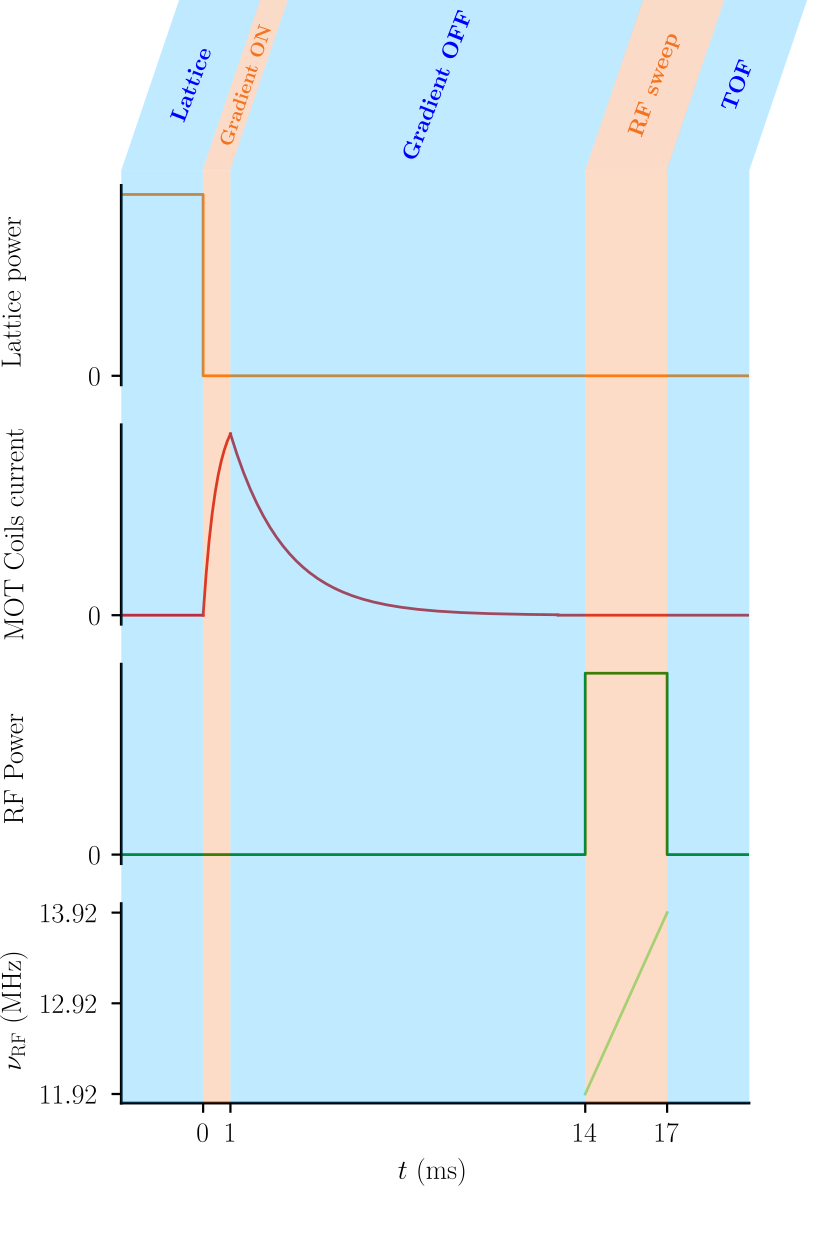
\includegraphics[width=0.8\textwidth]{Fig/Chapter5/displacement_sequence.png}
    \caption{Experimental sequence to shift the entire momentum distribution so that the $\kmf$ tails fall unto the $\He$ detector.}
    \label{fig:displacement_sequence}
\end{figure}

\subsection{Benchmarking with 3D lattice gases momentum distribution}

To test that our method does not induce any distortion of the momentum distribution, we benchmark it with 3D lattice gas momentum distribution slightly above the Mott critical point so that the momentum distribution has a wide background but still sharp diffraction peaks. This allows to check for distortion at high momentum values, while making more precise measurements with the narrow diffraction peaks \NOTE{vraiment pas ouf}.





\section{Experimental study}

\subsection{Measurement of the temperature}

\subsection{First extracted values of the Tan's contact}

\subsection{Comparison with QMC calculations}

\section{Discussion of the preliminary results}

% \chapterimage{}

\chapter*{Conclusion}

\label{chap:conclusion}
\addcontentsline{toc}{chapter}{\nameref{chap:conclusion}}


\fancyhead[LO]{\sffamily\bfseries Conclusion} % Print the nearest section name on the left side of odd pages
\fancyhead[RE]{\sffamily\bfseries Conclusion} % Print the current chapter name on the right side of even pages

The central result of this thesis is the observation of \kmk pairs in the quantum depletion of a weakly-interacting lattice Bose gas. Most of the work I did during my PhD was oriented towards that goal. This measurement was the next step in our task of fully characterizing the correlations across the superfluid-to-Mott insulator transition after the first two works \cite{carcy2019momentum,cayla2020} conducted by the former PhD students Hugo Cayla and Cécile Carcy that focused on the local correlations, respectively deep in the Mott regime and in the superfluid region. 

The first work that I conducted during my PhD is the study the two-body collisions halos \cite{tenart2020two} as a means to complete the previous benchmarking work \cite{cayla2018single} to certify that the measured atomic distribution faithfully represents the in-trap momentum distribution at the level of individual atoms. We devised a simple theoretical model predicting the number of atoms in the collision halos that we validated experimentally by measuring this number for large number of atoms loaded in the lattice. Extrapolating the predictions of the simple model to the low atom numbers usually used in our experiments, we could show that two-body collisions can be safely neglected, proving that our experiment is suited to probe correlations between individual particles. A second work aimed at studying the adiabatic preparation of the gas in the vicinity of the Mott transition \cite{carcy2021}. Led by Cécile Carcy in collaboration with the theoretician Tommaso Roscilde, it has been completed around the middle of my PhD, concluding the series of experiment aiming to prove that our experiment properly simulates the Bose-Hubbard model. In particular, this work showed that it is possible to adiabatically approach the Quantum Critical Point of the superfluid-to-Mott insulator transition at finite entropy, \ie without creating excitations, contrary to the $T=0$ case where this is expected to be impossible. This work then sets the ground for the study of correlations across the superfluid-to-Mott insulator transition that we defined as one of our main point of interest in the introduction to this manuscript.

Our team had attempted before at revealing the pairing mechanism associated to the quantum depletion without success. We identified the low detection efficiency ($\sim 10-15 \%$) as a central issue and thus we decided to implement a two-photon Raman transfer to improve the detection efficiency. Building and testing the Raman transfer was the second main project of my PhD. 

It was more or less at this time that the Covid-19 pandemic hit, forcing us to leave the lab and stay at home. I used this period away from the lab room to develop the algorithm to compute the anomalous correlation function $\gtwo_A$ (to look for the \kmk correlations). I tested and troubleshot this algorithm at first with simulated data and in a second time with the data from the earlier project on the collision halos (in which classical \kmk correlations can be observed in the frame of the center of mass of each halo). 

We started the measurement campaign for the \kmk correlations a few months after the end of first lockdown and were able to observe first experimental signals. We then performed experiments to investigate the role of temperature and of atoms number on the pairing signal and to compare pair correlations with the bunching effect. These measurements provided strong evidences that the observed \kmk correlations were the expected signature of quantum coherences built by atom pairs as a result of interactions. Several features associated with $T=0$ quantum coherences induced by the pairs could be observed and we propose an interpretation in analogy with two-mode squeezed states in Quantum Optics. 

In addition, we observed $\gtwo_A (\bm{0}) \gg \gtwo_N (\bm{0})$, violating the Cauchy-Schwarz inequality, once again signaling the quantum nature of the correlation signal, and finally measured relative number squeezing between modes $\bm{k}$ and $-\bm{k}$. These last two measurements constitute a first step towards demonstrating the presence of entanglement in the many-body equilibrium state of our system. This notably opens the way to characterizing squeezing and entanglement with \textbf{continuous} variables (here the momentum), extending such studies beyond \textbf{discrete} spin variables as mostly done so far.

In a nutshell, we were able to report the first observation of \kmk correlations in an \textbf{at-equilibrium} system, resulting from the interplay between quantum fluctuations and interactions, confirming the 60 years old prediction of Bogoliubov and Lee-Huang-Yang. Interestingly, one of the motivations to observe this signal laid in its conceptual simplicity and the existence of the well-rounded Bogoliubov theory describing it, giving us a general frame to interpret the experimental data. However, the presence of the optical lattice represents an already significant change from the homogeneous Bogoliubov theory and makes theoretical approaches much more complicated and to this day missing. While many of our observations are consistent with Bogoliubov theory, we observed that it notably fails to quantitatively explain the number of detected pairs. This means that our experiment starts to qualify as a quantum simulator as defined in the introduction, even though new theories might emerge in the near future to explain these results as the complexity of the system is still manageable. 

Building up on the quantum simulation aspect, this result is also of great importance for our future experiments as it shows that our experiment is capable of detecting non-local \kmk correlations (we had only observed close-by \kk correlations before), hinting at a possible detection of more complex and hard to predict correlation patterns, notably close the Quantum Critical Point of the Mott transition, that would be a big step towards understanding the physics of strongly interacting many-body systems. This also confirms that we could detect \kmk correlations in Cooper pairs and help understanding the physics of superconductivity with future experiments with fermionic $^3 \rm{He}^*$.

In parallel, I also spent a significant amount of time working on the project of measuring Tan's contact in 1D gases, in collaboration with Hepeng Yao and his supervisor Laurent--Sanchez Palencia from Centre de Physique Théorique at Ecole Polytechnique. This work also falls into the general goal of studying many-body interacting systems with a complementary approach to correlation functions, \ie measuring high momentum tails revealing the presence of contact interactions. We implemented a solution to increase the momentum range of the detector by using a magnetic gradient to shift the entire momentum distribution and access the high momentum region, and were able to observe a $\kmf$ decay on various data sets. While the qualitative evolution of the contact with temperature and interaction strength is consistent with theory, there is a large discrepancy with the QMC calculations that remains to this day unexplained and should be the subject of future experiments. Obtaining an agreement with theory would be of primary importance to show that the momentum density at high $k$ can be used to properly characterize the different regimes and crossovers between them in interacting 1D gases.

\section*{Outlooks}

Our measurements of \kmk correlations have voluntarily left constant the lattice depth. An immediate way of pushing these measurements further (that we have already started working on) is to monitor the pairing while progressively increasing the lattice depth. As $U/J$ increases, and with it the strength of the interactions, we should reach a point at which the Bogoliubov approximation is not valid anymore. It would then be interesting to see how this effect translates to the \kmk correlation signal. As mentioned earlier, we notably expect that more complex correlation patterns may appear as the strength of the interactions increases, effectively involving more than 2 particles. These kind of complex correlations are expected to be particularly important at the Quantum Critical Point of the superfluid-to-Mott insulator transition. A short-mid range prospect would then be to develop new data analysis techniques to measure higher order correlation functions, test them in simple cases like by measuring bosononic bunching with more than 2 particles, and finally use them in experimental data progressively closer to the Quantum Critical Point. As obtaining a good enough signal to noise ratio to measure a $n$-th order correlation function gets increasingly difficult as $n$ increases, we would need to take large amount of data at the Quantum Critical Point. This prospect is particularly exciting as no theory predicts what should happen in terms of momentum space correlations at the Quantum Critical Point, making this measurement a true quantum simulation. 

In addition, our observation of the violation of the Cauchy-Schwarz inequality would be enough to obtain the important result of proving the presence of entanglement in momentum space in many-body equilibrium systems if we were able to measure the correlator  $\langle a^{\dagger}_{\bm k} a_{-\bm k} \rangle$ and show that it is negligible, as in Bogoliubov theory. Improving our experimental setup to have the lattice beams required to perform atomic interferometry and measure this correlator then constitutes another interesting outlook.

Another short term objective is to further investigate the discrepancy between the experimental data and the QMC calculations for the measurement of Tan's contact, notably by taking additional data using the newly added two-photon Raman transfer. We hope that the increased detection efficiency would help us being less sensitive to possible effects of the $m_j=0$ impurities while reducing the number of non-transferred $m_j=1$ atoms. While these atoms are supposed to be prevented from falling on the detector thanks to a strong magnetic gradient kick, we observed that there could be unwanted dynamics such as uncontrolled transfer to the $m_j=0$ state that could perturb our measurement. This measurements might then help us to identify eventual problems in the experiment or in the way that we compare our data to the theory.

Finally, a more long term prospect would be to improve the experimental setup to bring the fermionic isotope of Helium, $^3\He$, to quantum degeneracy. This would open the way to study a whole new kind of physics with the great momentum space resolution of our detector. It would be particularly interesting to study the physics of the BEC-BCS transition and directly measure \kmk correlations in a Cooper pair. To do so, we would first need to identify a usable Feshbach resonance to create the Cooper pairs as there have currently not been a proper investigation of the existence of Feshbach resonance in $^3\He$. 

\renewcommand{\thefigure}{1}
\begin{figure}[h!]
    \centering
    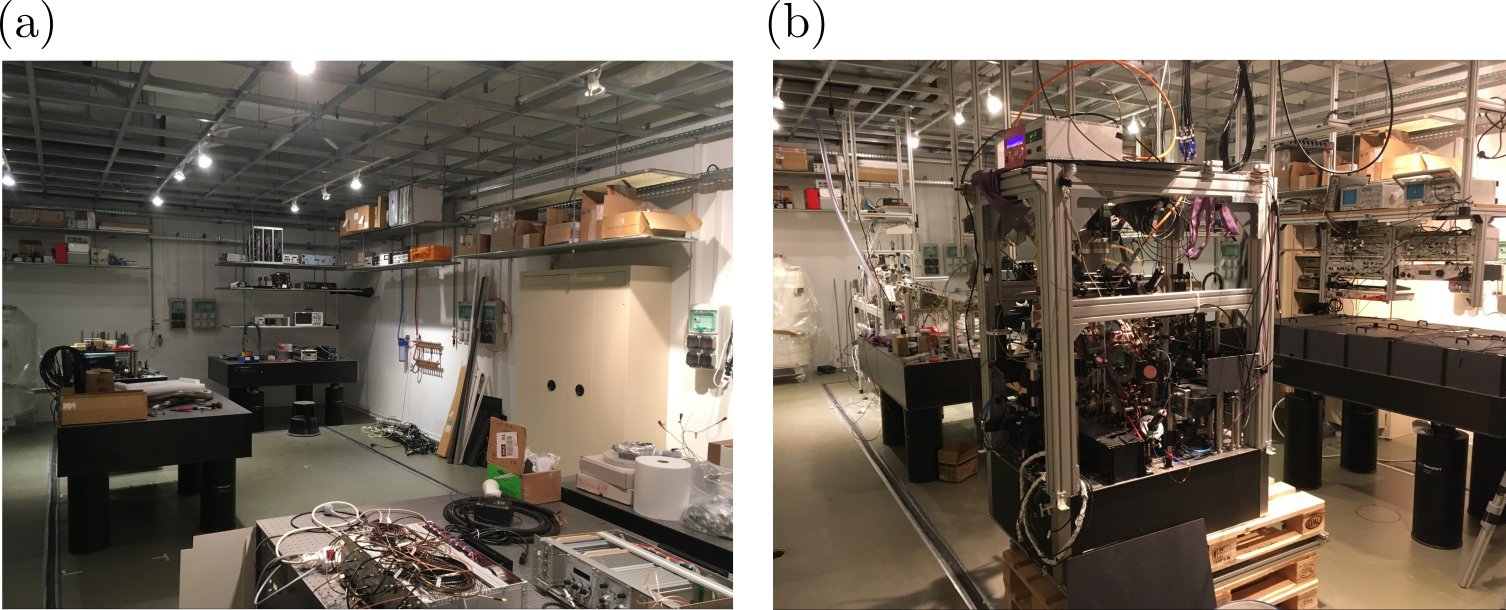
\includegraphics[width=0.95\textwidth]{Fig/Conclusion/before_after.png}
    \caption[The new experiment room]{The new experiment room. (a) Before moving in, with only a few optical tables left by the previous occupants of the room. (b) After moving in.}
    \label{fig:before_after}
\end{figure}

Actually, the lab room in which all the experiments of this thesis were conducted was starting to get packed, and adding the new equipment to cool down a new atomic species would have barely left enough space in the room for a PhD student. This last year, we took a first (but big!) step towards the installation of $^3\He$ in our experiment by moving the entire apparatus to a new bigger room a few steps down the corridor (see Fig.-\ref{fig:before_after}), giving us plenty of additional space. At the moment that I am writing this manuscript, we managed to get the experiment back to its working state and were able to produce BECs and should be able to resume taking data soon. I would like to end this manuscript with one last figure (\ref{fig:SC_moving}) which is of my favorite picture of my time as a PhD student, showing the Helium Lattice team in the perilous process of moving the science chamber to the new room, in which I hope it will serve to make many beautiful experiments in the years to come.



\renewcommand{\thefigure}{2}

\begin{figure}
    \centering
    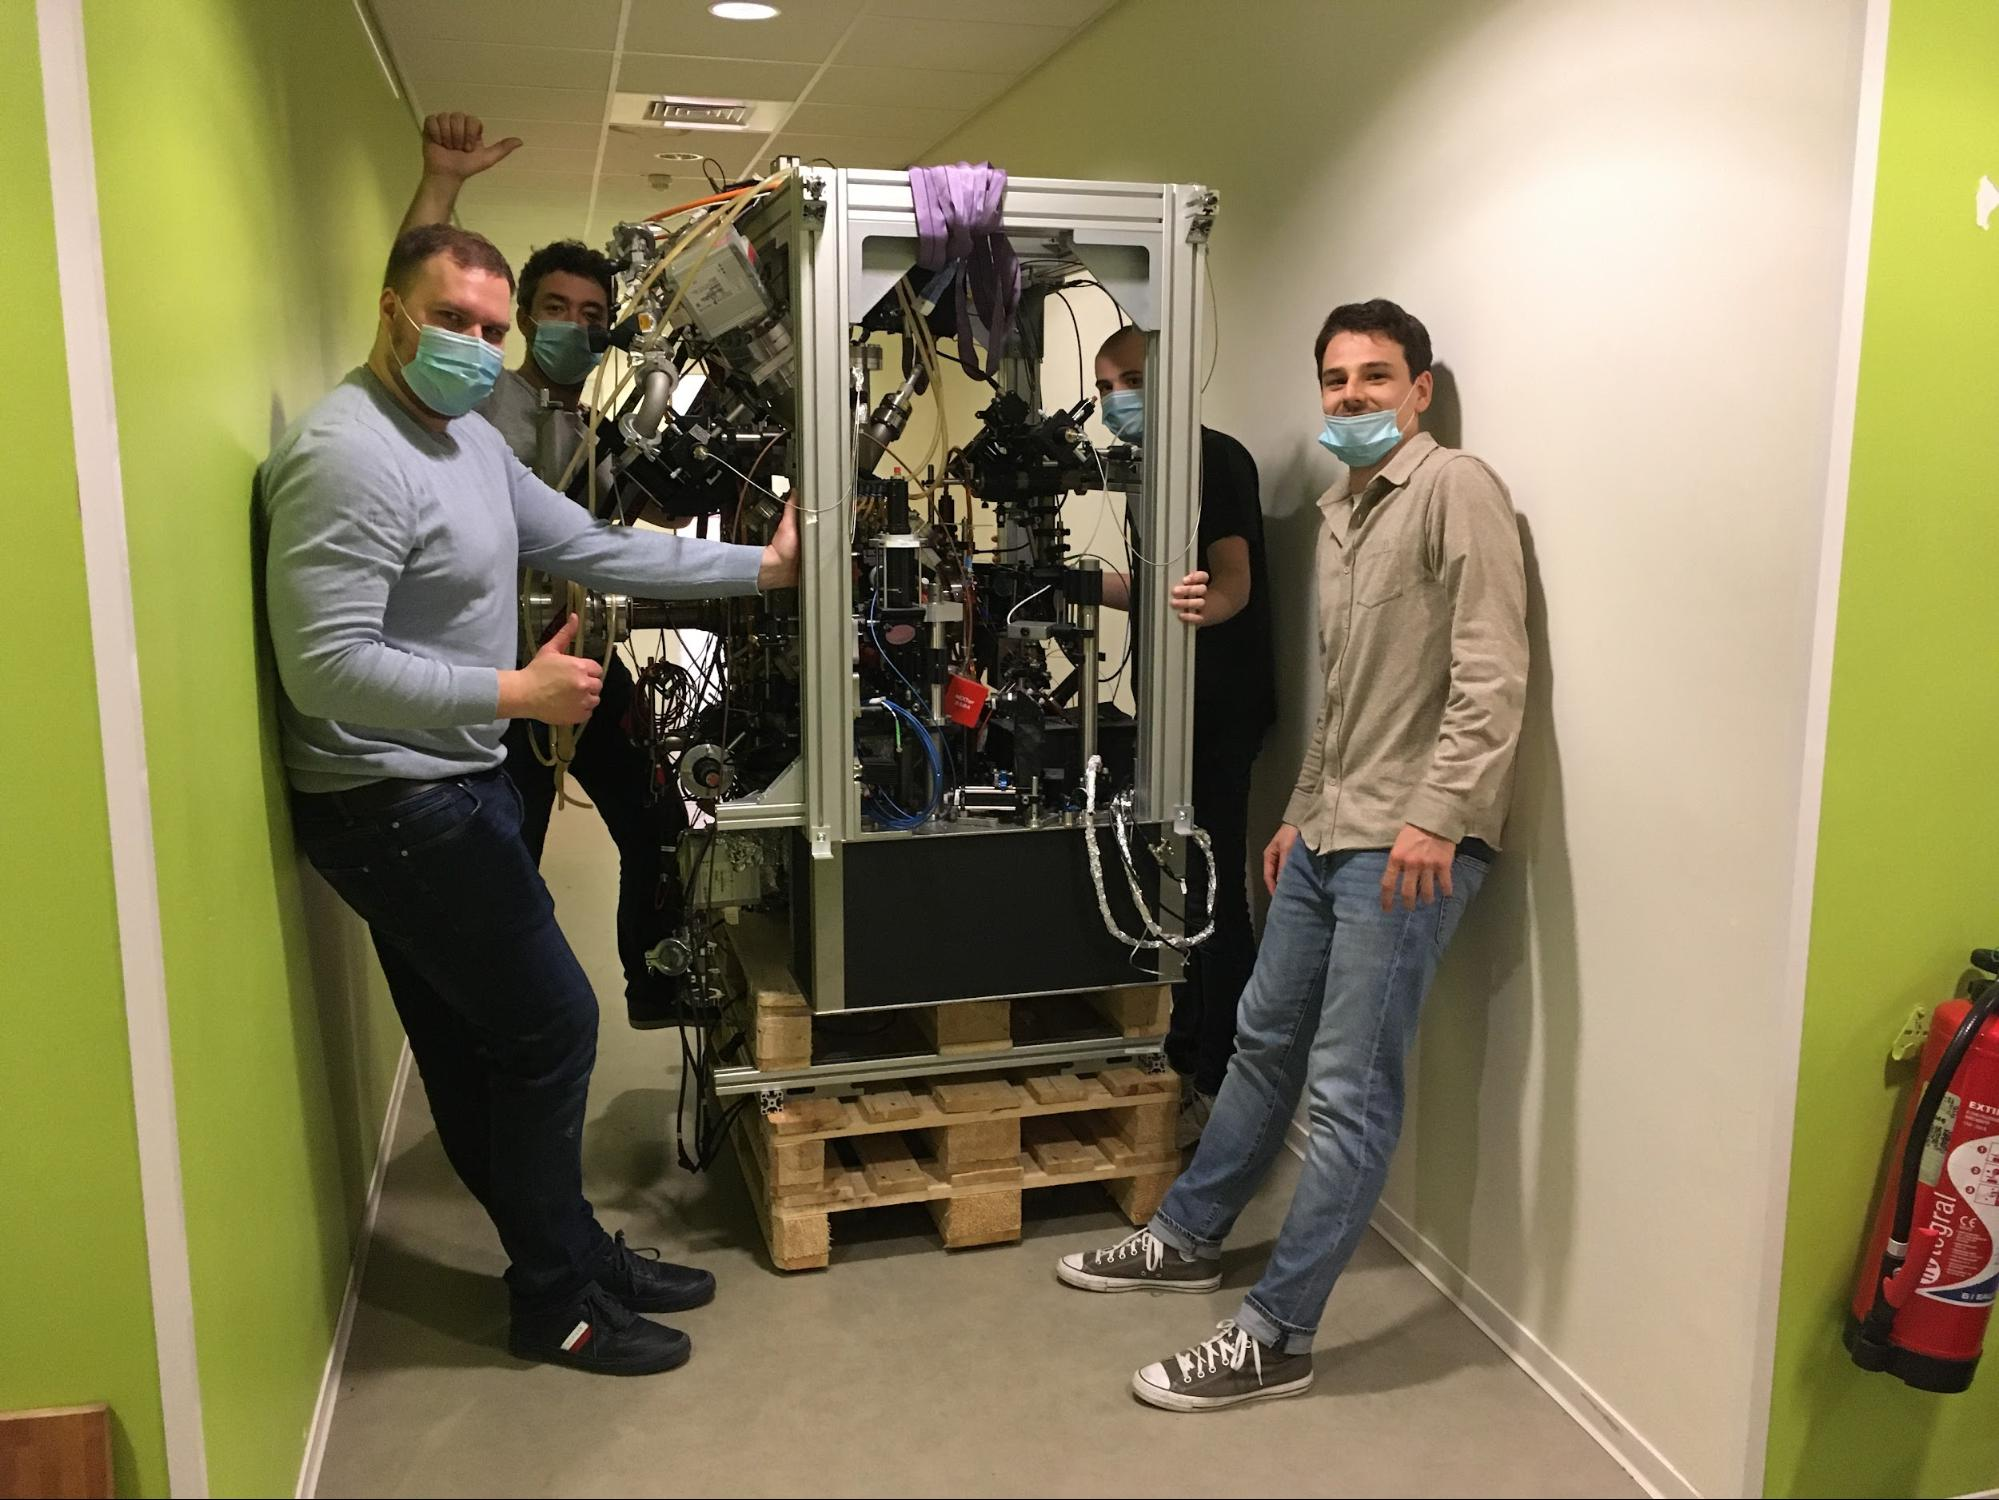
\includegraphics[width=0.8\textwidth]{Fig/Conclusion/SC_moving.jpg}
    \caption{The Helium Lattice team with the Science Chamber, moving from the old room to the new one.}
    \label{fig:SC_moving}
\end{figure}





\setlength{\parskip}{\parskipinitial}
%\usechapterimagefalse

\addcontentsline{toc}{chapter}{Bibliographie}
\fancyhead[LO,RE]{\sffamily\normalsize\bfseries Bibliographie}

\bibliography{sample}



\end{document}
